%% This file explains the options available to you for editing the file
%% main.tex.

%% The commands in this file allow you to specify options such as
%% spacing, double-sided printing, a draft copy, etc.   By default, 12pt
%% and lgrind are included; lgrind is the 2e style for including code in
%% your thesis.

%% \documentclass[12pt]{mitthesis}
%% \usepackage{lgrind}
%% \pagestyle{plain}

%% You can add options in the documentclass line as follows:

%% 	o  singlespace
%% 	\documentclass[12pt,singlespace]{mitthesis}
	
%% 	o  twoside
%% 	\documentclass[12pt,twoside]{mitthesis}

%% 	o  draft   (make sure to change the pagestyle to drafthead as well)
%% 	\documentclass[12pt,draft]{mitthesis}
%% 	\usepackage{lgrind}
%% 	\pagestyle{drafthead}

%% 	o vi   (for course vi and course viii theses)
%% 	\documentclass[12pt,vi]{mitthesis}

%% Any options you would use for report.sty will work here as well.


%% You should not need to change the first three lines and last two lines
%% below.  Be sure to include an \include command for each file you are
%% including in your thesis.
  
%% % -*-latex-*-
% 
% For questions, comments, concerns or complaints:
% thesis@mit.edu
% 
%
% $Log: cover.tex,v $
% Revision 1.9  2019/08/06 14:18:15  cmalin
% Replaced sample content with non-specific text.
%
% Revision 1.8  2008/05/13 15:02:15  jdreed
% Degree month is June, not May.  Added note about prevdegrees.
% Arthur Smith's title updated
%
% Revision 1.7  2001/02/08 18:53:16  boojum
% changed some \newpages to \cleardoublepages
%
% Revision 1.6  1999/10/21 14:49:31  boojum
% changed comment referring to documentstyle
%
% Revision 1.5  1999/10/21 14:39:04  boojum
% *** empty log message ***
%
% Revision 1.4  1997/04/18  17:54:10  othomas
% added page numbers on abstract and cover, and made 1 abstract
% page the default rather than 2.  (anne hunter tells me this
% is the new institute standard.)
%
% Revision 1.4  1997/04/18  17:54:10  othomas
% added page numbers on abstract and cover, and made 1 abstract
% page the default rather than 2.  (anne hunter tells me this
% is the new institute standard.)
%
% Revision 1.3  93/05/17  17:06:29  starflt
% Added acknowledgements section (suggested by tompalka)
% 
% Revision 1.2  92/04/22  13:13:13  epeisach
% Fixes for 1991 course 6 requirements
% Phrase "and to grant others the right to do so" has been added to 
% permission clause
% Second copy of abstract is not counted as separate pages so numbering works
% out
% 
% Revision 1.1  92/04/22  13:08:20  epeisach

% NOTE:
% These templates make an effort to conform to the MIT Thesis specifications,
% however the specifications can change. We recommend that you verify the
% layout of your title page with your thesis advisor and/or the MIT 
% Libraries before printing your final copy.
\title{Analysis of Beauty Quark Hadronization in Vacuum and Quark-Gluon Plasma with CMS}

\author{Zhaozhong Shi}

%\author{B. A., in Physics, University of California, Berkeley (2016)}

\prevdegrees{B.A., University of California, Berkeley (2016)}

% If you wish to list your previous degrees on the cover page, use the 
% previous degrees command:
%       \prevdegrees{A.A., Harvard University (1985)}
% You can use the \\ command to list multiple previous degrees
%       \prevdegrees{B.S., University of California (1978) \\
%                    S.M., Massachusetts Institute of Technology (1981)}
\department{Department of Physics}

% If the thesis is for two degrees simultaneously, list them both
% separated by \and like this:
% \degree{Doctor of Philosophy \and Master of Science}
\degree{Doctor of Philosophy in Physics}

% As of the 2007-08 academic year, valid degree months are September, 
% February, or June.  The default is June.
\degreemonth{September}
\degreeyear{2021}
\thesisdate{September 5, 2021}

%% By default, the thesis will be copyrighted to MIT.  If you need to copyright
%% the thesis to yourself, just specify the `vi' documentclass option.  If for
%% some reason you want to exactly specify the copyright notice text, you can
%% use the \copyrightnoticetext command.  
%\copyrightnoticetext{\copyright IBM, 1990.  Do not open till Xmas.}

% If there is more than one supervisor, use the \supervisor command
% once for each.
\supervisor{Yen-Jie Lee}{Associate Professor}

% This is the department committee chairman, not the thesis committee
% chairman.  You should replace this with your Department's Committee
% Chairman.
\chairman{Nergis Mavalvala}{Associate Department Head of Physics}

% Make the titlepage based on the above information.  If you need
% something special and can't use the standard form, you can specify
% the exact text of the titlepage yourself.  Put it in a titlepage
% environment and leave blank lines where you want vertical space.
% The spaces will be adjusted to fill the entire page.  The dotted
% lines for the signatures are made with the \signature command.
\maketitle

% The abstractpage environment sets up everything on the page except
% the text itself.  The title and other header material are put at the
% top of the page, and the supervisors are listed at the bottom.  A
% new page is begun both before and after.  Of course, an abstract may
% be more than one page itself.  If you need more control over the
% format of the page, you can use the abstract environment, which puts
% the word "Abstract" at the beginning and single spaces its text.

%% You can either \input (*not* \include) your abstract file, or you can put
%% the text of the abstract directly between the \begin{abstractpage} and
%% \end{abstractpage} commands.

% First copy: start a new page, and save the page number.
\cleardoublepage
% Uncomment the next line if you do NOT want a page number on your
% abstract and acknowledgments pages.
% \pagestyle{empty}
\setcounter{savepage}{\thepage}
\begin{abstractpage}
% $Log: abstract.tex,v $
% Revision 1.1  93/05/14  14:56:25  starflt
% Initial revision
% 
% Revision 1.1  90/05/04  10:41:01  lwvanels
% Initial revision
% 
%
%% The text of your abstract and nothing else (other than comments) goes here.
%% It will be single-spaced and the rest of the text that is supposed to go on
%% the abstract page will be generated by the abstractpage environment.  This
%% file should be \input (not \include 'd) from cover.tex.
An analysis of fully reconstructed $B^0_s$ and $B^+$ mesons decay into $J/\psi$ and strange hadrons using Compact Muon Solenoid (CMS) Experiment 2017 pp dataset and 2018 PbPb data at the center of mass energy per nucleon $\sqrt{s_{NN}} = 5.02$ TeV at the Large Hadron Collider (LHC) is presented. We apply machine learning techniques along with multivariate analysis to obtain significant B-meson signals and extend the kinematic regime of B-meson measurements with higher precision. In our analysis, $B^0_s$ signal of greater than 5 $\sigma$ significance is observed for the first time in heavy-ion collisions. The measured $B^0_s$/$B^+$ ratio in PbPb along with pp references are compared with theoretical model predictions. These results will help elucidate the beauty quark hadronizaton mechanisms in vacuum and quark-gluon plasma at the LHC energy. Significant B-meson signals have also been observed at low very $p_T$ and high multiplicity in pp collisions, which will allow us study beauty hadrochemistry in small systems and energy loss mechanism in the future. 
\end{abstractpage}

% Additional copy: start a new page, and reset the page number.  This way,
% the second copy of the abstract is not counted as separate pages.
% Uncomment the next 6 lines if you need two copies of the abstract
% page.
% \setcounter{page}{\thesavepage}
% \begin{abstractpage}
% % $Log: abstract.tex,v $
% Revision 1.1  93/05/14  14:56:25  starflt
% Initial revision
% 
% Revision 1.1  90/05/04  10:41:01  lwvanels
% Initial revision
% 
%
%% The text of your abstract and nothing else (other than comments) goes here.
%% It will be single-spaced and the rest of the text that is supposed to go on
%% the abstract page will be generated by the abstractpage environment.  This
%% file should be \input (not \include 'd) from cover.tex.
An analysis of fully reconstructed $B^0_s$ and $B^+$ mesons decay into $J/\psi$ and strange hadrons using Compact Muon Solenoid (CMS) Experiment 2017 pp dataset and 2018 PbPb data at the center of mass energy per nucleon $\sqrt{s_{NN}} = 5.02$ TeV at the Large Hadron Collider (LHC) is presented. We apply machine learning techniques along with multivariate analysis to obtain significant B-meson signals and extend the kinematic regime of B-meson measurements with higher precision. In our analysis, $B^0_s$ signal of greater than 5 $\sigma$ significance is observed for the first time in heavy-ion collisions. The measured $B^0_s$/$B^+$ ratio in PbPb along with pp references are compared with theoretical model predictions. These results will help elucidate the beauty quark hadronizaton mechanisms in vacuum and quark-gluon plasma at the LHC energy. Significant B-meson signals have also been observed at low very $p_T$ and high multiplicity in pp collisions, which will allow us study beauty hadrochemistry in small systems and energy loss mechanism in the future. 
% \end{abstractpage}

\cleardoublepage

\section*{Acknowledgments}

%This is the acknowledgements section. You should replace this with your own acknowledgements.

Today, sitting in front of my Macbook and writing up my PhD thesis, I am recalling the nice memory over the past 5 years of my academic and research journey at MIT. I have overcome countless challenges and seized every opportunity. I have absorbed plenty of knowledge like nutrients and lead work alcoholic life. I used to work more than many hours, particularly when deadlines are approaching. I am glad that I have overcome countless of deadlines and managed to finish most of my tasks on time during my graduate studies. Because of my hard work and achievements, during my graduate studies at MIT, I have been awarded the NSF-GRFP and DOE SCGSR fellowships. While I am proud of my academic and research accomplishments, the more importance things are love and friendship. I have been to many memorable places around the world and met many interesting people. They have taught me more than I can learn from papers, lectures, and experiments. I owed them a lot and am indebted to everyone for their influences on me. Without them, I will not be able to finish this work and reach my current maturity.

On the cloudy afternoon of February 12, 2016, I was anxiously waiting for my graduate admission decisions. At around 2pm when I am returning home from Berkeley, I received my acceptance to MIT from the MIT Department of Physics Coordinator Catherine Modica. At that moment, I was still on my BART from UC Berkeley back to San Francisco. I was very excited and immediately called my family to share this great news. I understood that this would be the start of my exciting career as a PhD candidate in Nuclear Physics research. Without thinking too much, I quickly accepted the offer and got ready to join MIT.

During the MIT Open House, I met a lot of amazing people. I first visited the MIT Heavy Ion Group and then made friends with many of my peers. I would really like to thank Constantin Weisser for his generous accommodation during the Open House. I met my future PhD advisor Professor Yen-Jie Lee and LNS director Bolek Wyslouch. I also met my fellow students at LNS such as Lauren Yates, Sangbaek Lee, and Yi Jia. They are all very nice and kind. We have spent our first three semesters together taking classes and discussing physics. Particularly, I want to mention Sangbaek that we used to discuss a lot about our life stories and future perspectives together. It was a quite memorable experience. I also frequently visited lattice QCD theorist Anthony Grebe. I still remembered the time we discussed physics questions, debated ideas, derive formulae at the Center for Theoretical Physics. He is a truly humble and kind person. I wish him to have a successful future career in theoretical particle physics.


As a resident of MIT Tang Hall, I met many interesting people. Here, I would like to thank Ali Fahimniya who also lived at Tang Hall for his first year. We often chat with each other during the cookies social in the Pappalardo Room. We shared our life experience and future plan. It turns out that we defended our PhD just a day apart from each other. 

Shortly after attending MIT, I decided to join the MIT Heavy Ion Group and pursued my scientific research career in Experimental High Energy Nuclear Physics as my PhD thesis topic for the next 5 years. Members of the MIT Heavy Ion Group have provided me with general supports and comprehensive guidance towards my PhD. Without them, I would not be able to overcome challenges and finish my thesis research projects. 


At the graduate student's office, my desk is located in the northwest corner. Senior members of faculties in our group offered me excellent training and many opportunities to become an independent researcher and build up my international reputation in the field. I would particularly like to thank Professor Yen-Jie Lee for his long and enduring support, both in research and life, for the past 5 years. He has provided me with many opportunities and ideas to carry out physics analysis and fought in the CMS collaboration to allow me to give talks in internationally recognized conferences. I am also deeply indebted to him for his care of my career development and letters of recommendation for fellowships and postdoctoral scholar positions. Thanks to his nurture, I have transformed from a student knowing almost nothing to become an independent researcher with some big-picture visions. I am also grateful to the MIT Heavy Ion Group leader Professor Gunther Roland for his generous supports to allow me to work on sPHENIX and EIC projects. His letters of recommendation and grant management advice helps me a lot to get my first postdoctoral position and become professional in developing leadership skills in academia. Both of them have provided me with opportunities to work at different places around the world such as MIT, Fermilab, BNL, and CERN. Aside from them, I appreciated the general academic etiquette and soft skills from Professor Bolek Wyslouch.


My fellow senior graduate colleagues in my group have influenced me a lot. First, the most senior graduate student Dragos Velicanus showed me around about our group and guided me through the basics. He also provided a lot of remarks on my fellowship applications. Then, Alex Barberi sat next to my office desk. We have worked together and talked about funny anecdotes. I also made acquittances with Ta-Wei Wang. He created the skimmed files for me to play with and answered me many technical questions in C$++$ programming and B mesons full reconstructions. As a newbie in the CMS analysis, I used to frequently bother Jing Wang in the analysis techniques and questions on codes. However, she still patiently guided and helped me until my confusion was gone. As the CMS spectra heavy flavor group leader, she also gave a lot of feedback and suggestions to validate the analyses. Ran Bi, whose research was on photon-jet studies, was a bit reserved but still kindly helped me a lot with CMS software and technical concepts for data processing and analysis. Kaya Tatar was a very nice and resourceful person. We used to discuss many physics and technical questions. Chris McGinn was one of my best friends at the MIT Heavy Ion Group. He provided me with a lot of technical assistance and helped me debug my codes. His help was very effective. I really appreciated that. We also debated many physics concepts and politics issues. Austin Baty was one of my buddies at CERN who used to share his experience in life and studies with me.  

Junior graduate students such as Michael Peters, Molly Taylor, and Gwang-Jun Kim were all very friendly and kind. I will never forget the time when Michael and I initiated the debate and keep on our position to try to convince with each other. I also enjoyed working with Gwang-Jun and still remember the moments we stay up many days and nights fighting to get the analysis from pre-approve to approval stage. I also would like to thank Molly for helping me look after my remaining items near my desks in the MIT office since I went to CERN. 


Staff members of our group were very professional and resourceful. Dr. Gian Michele guided me through my analysis and gave me useful feedback for my first Quark Matter talk. I have learned a lot from him in the first two years of my PhD studies. Dr. Camellia Mironov has guided me through the CMS collaboration bureaucracy and went through the procedures to present and publish papers. Dr. George Stephans has provided me with many suggestions in MC simulations, technical questions, physics concepts, and computing knowledge. Dr. Christoph Roland has shared me with a lot of heavy-ion physics anecdotes, career development stories, detector hardware knowledge, software development skills, and analysis techniques. I would also like to thank Dr. Ivan Cali for his suggestions in windows codes programming, software development, and product design. Finally, I would like to thank the administrative assistant Anna Convertino for handling my travel and paperwork.  

%Faculty Yen-Jie; emphasize. 

I would also like to thank my fellow students at the PPC including Dr. Dylan Hsu, Dr. Brandon Allen, Dr. Sid Narayanan, Dr. Stephanie Brandt, and Jeff Krupa. They are all my good friends. We treated each other like brothers and made fun of each other. I still remembered I visited the PPC office almost every day and shared how my day was with them. They used to say I would not be able to graduate in 6 years but I did manage to get my PhD within 5 years, which surprised them a lot. Jeff was also my buddy. We used to go out for lunch regularly and walked along the beach every semester. I missed them all very much!

Aside from that, many other professors at MIT have helped me a lot academically and professionally. I would particularly thank my academic advisor Professor Lindley Winslow. She is very kind, considerate, and helpful. She gave me very good advice on fellowship applications, courses selections, degree preparation, and postdoc tips. My graduate career has become much smoother and planned thanks to her kind suggestions. In addition, I would like to thank Professor Iain Stewart, Richard Milner, and Krishna Rajagopal for occasional discussions. I would also like to thank Professor Barton Zwiebach for serving as the reader in my PhD thesis committee and provided me with some useful feedback about my defense and presentation.

Outside MIT, I have also met many senior sages who have given me a lot of wisdom. As a member of sPHENIX calorimetry test beam crews at Fermilab, I met Dr. Craig Woody and worked with him during the first days in 2017. After that, he has been my mentor for the past 5 years and served as my laboratory scientist for the Electron-Ion Collider Electromagnetic Calorimeter project in my DOE SCGSR award. Moreover, he has written many letters for me and provided me with a lot of resources for career development. I am very thankful for his support. I also met Dr. Jin Huang and received many technical and analysis guidances for my sPHENIX EMCAL, heavy flavor simulation, and EIC EMCAL projects. I would also like to thank Dr. John Haggerty for his creative training during my shift at Fermilab in 2017 and 2018. At CERN, I felt very fortunate to work with Professor Mario Sitta on ALICE ITS project. He was my best friend during my stay in France and has kindly helped me move my personal items around with his car and debug my programs. Without him, my stay at CERN could be very miserable. I would also like to express my sincere gratitude to my collaborator Nuno Leonardo at LIP in Portugal. Collaborating on the B-meson analysis, he has provided me with many concrete solutions to improve the analysis, ideas to overcome the challenges from the CMS collaboration, and workforce supports to complete part of the projects. He has saved this analysis many times. His efforts, along with my hard work, finally managed to make it possible and become part of my thesis. Without his support, my analysis would be stuck in many steps and may not be able to advance to the current ready for submission stage. His urgent emails and slack messages were still clearly remembered in my mind. I also met Ming Liu during the Fermilab test beam shift and ALICE ITS commissioning at CERN. We worked together at that time. We will work together as a postdoc and a mentor for the next three years. Finally, I am very lucky to have a chance to have a nice lunch with Professor James Bjorken. I have really learned many stories in the great old days of the Golden Age of particle physics and about the fun of physics with him. I also got to know his recent research interests and received some career advice from him. It was my great honor to chat with this great mind.

In addition to my mentors, colleagues, and friends, I would also like to thank my family. During the COVID-19 pandemic in the last year of my PhD studies, I stayed at home and received a lot of care from them. I was able to really focus on finishing my thesis research and became much more productive than in the past 3 years. I am really grateful to their unconditional love. 

Finally, I would really like to especially thank my significant other Zhixin Lai in this paragraph. Since I met her in February 2020, she has been my soul mate. We shared everything in our life, worked together, and have learned a lot from each other. When we experienced obstacles and failures, we cheered each other up. When we saw opportunities and success, we expressed our happiness with each other and celebrated our achievements on the phone. She has helped me a lot in my career and gave me many helpful suggestions to improve the writing of my fellowship applications, job hunting, and PhD thesis. After almost a year and a half since we knew each other, the US-Canadian border was finally open. I finally had a chance to meet her in person. We sat together and prepared my thesis defense. Her company with me in my PhD thesis defense and my celebration dinner made it the most memorable day in my life. She has made me a more complete and mature person. I am indebted to her sincere love and really hope to experience more ups and downs with her in the future.



%BNL: Craig Woody. Jin Huang. John Haggerty.

%LANL: ming

%Fermilab:

%SLAC: BJ


%CERN: Marrio Sitta, Ivan, Markus Keil, 



%I lived at Tang Hall and met many amazing people 


%Grad Lounge guys,

%PGSC Pizza social guys

%PPC bros

%MIT Heavy Ion group members



I am sorry that I may not be able to exhaust the list of everyone. But I really believe that I have learned a lot from all of you. I am sincerely grateful to your influences and friendships on my growth as a scientist and a person. 

%%%%%%%%%%%%%%%%%%%%%%%%%%%%%%%%%%%%%%%%%%%%%%%%%%%%%%%%%%%%%%%%%%%%%%
% -*-latex-*-

%% \pagestyle{plain}
%%   % -*- Mode:TeX -*-
%% This file simply contains the commands that actually generate the table of
%% contents and lists of figures and tables.  You can omit any or all of
%% these files by simply taking out the appropriate command.  For more
%% information on these files, see appendix C.3.3 of the LaTeX manual. 
\tableofcontents
\newpage
\listoffigures
\newpage
\listoftables
%% 
%% This is an example first chapter.  You should put chapter/appendix that you
%% write into a separate file, and add a line \include{yourfilename} to
%% main.tex, where `yourfilename.tex' is the name of the chapter/appendix file.
%% You can process specific files by typing their names in at the 
%% \files=
%% prompt when you run the file main.tex through LaTeX.
\chapter{Introduction}

\section{The Standard Model of Particle Physics}

%Physics is the research of relationship between space and time and energy and matter. Physicists enjoy searching for symmetries and consideration laws in nature. They develop elegant mathematical formulations to describe the beauty of the nature and predict or explain the experimental results and observed phenomena. 

There are four known fundamental forces in nature: gravitational force, electromagnetic force, strong force, and weak force. The gravitation force describes the interaction between two massive objects. The electromagnetic force describes the interaction between electrically charged objects. The strong force describes the interaction between nucleons. The weak force describe the radioactive decay of particles. The Standard Model (SM) of Particle Physics, first proposed and named by physicist Steven Weinberg in the 1960s \cite{StandardModel}, is based on theoretical frame of relativistic quantum field theory with a gauge symmetry of $SU(3) \times SU(2) \times U(1)$ \cite{SMTheory}. It unifies the electromagnetic and weak interactions and include the strong interaction into a theory and describes all particles participating in these interactions. The ingredient of the standard model are leptons, quarks, gauge bosons, and the Higgs boson shown in Figure~\ref{fig:SMParticle}.

\begin{figure}[hbtp]
\begin{center}
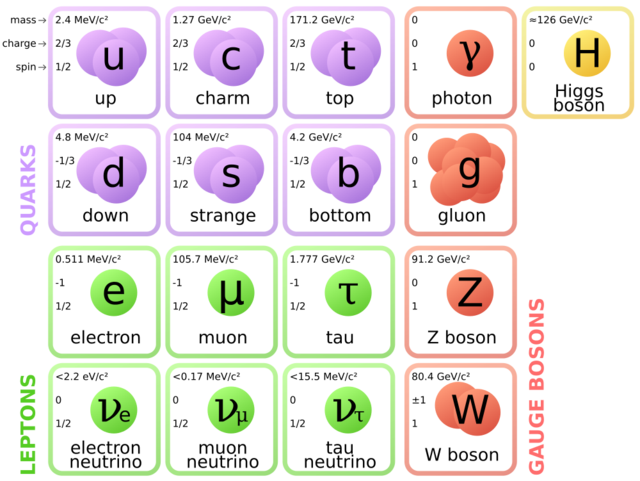
\includegraphics[width=0.50\textwidth]{Figures/Chapter1/SMParticles.png}
\caption{The 17 elementary particles, including 6 leptons, 6 quarks, 4 gauge bosons, and the Higgs boson, and their basic properties, such as mass, electric charge, spin, in the Standard Model of Particles Physics are shown above.}
\label{fig:SMParticle}
\end{center}
\end{figure} 


There are 19 parameters in the Standard Model: 6 quark masses, 3 lepton masses, 3 coupling strengths, 4 angles in the Cabibbo?Kobayashi?Maskawa Matrix, Higgs mass, vacuum expectation value, and QCD vacuum angle. These parameters are determined from the experiments. Physicists perform calculations based on the Standard Model and predict the cross section of different processes in high energy physics experiments. Since it is proposed in the 1970s, the Standard Model has been tested extensively in countless high-energy physics experiments. Its prediction holds for all of them with very few exceptions. The Standard Model consists of two sectors: the Electroweak theory (EW) and Quantum Chromodynamics (QCD). The Lagrangian of the Standard Model can be written as the sum of EW and QCD: $\mathcal{L_{SM}} = \mathcal{L_{EW}} + \mathcal{L_{QCD}}$ 


\section{Quantum Chromodynamics}

\subsection{QCD Lagrangian}

QCD, a non-abelian gauge theory with $SU(3)$ symmetry, is the theory for the strong interaction between quarks and gluons. The QCD Lagrangian is shown as follows:


\begin{equation}
\mathcal{L_{QCD}} = \bar \Psi^i i (\slashed{D})_{ij} \Psi^j - m  \bar \Psi^i \Psi_i - \frac{1}{16\pi^2} G^{\mu\nu}_{a}G_{\mu\nu}^{a}
\end{equation}

Where 

\begin{equation}
\slashed{D} = \gamma^\mu \partial_\mu - i g_s \frac{\lambda}{2}  \gamma^\mu A_\mu
\end{equation}

\begin{equation}
G^{\mu\nu}_{a} = \partial^\mu A^\nu_{a} - \partial_{\nu} A^\mu_{a} + g_s f_{abc} A^\mu_b A^\nu_c 
\end{equation}

Here, $\lambda$ are the Gell-Mann Matrices. $f_{abc}$ is the structure of constant of $SU(3)$. $A^\mu$ is the eight gluon field. $g_s$ is the strong coupling constant. The color indices $i$ and $j$ run from 1 to 3, which stands for 3 colors: red, blue, and green. The gluon field indices $a$, $b$, and $c$ run from 1 to 8, standing for the 8 gluon state (Gluon octet as the combination of 3 color and 3 anticolor: $3 \times \bar 3 = 1 \oplus 8$) living in the adjoint representation of $SU(3)$ of color.  



\subsection{Asymptotic Freedom}

The running of the strong coupling constant $\alpha_s = \frac{g_s^2}{4\pi}$ according to the 1-loop calculations in the renomalization theory \cite{QCDRunning} is shown as follows

\begin{equation}
\alpha_{s} (Q^2) = \frac{12\pi}{(11 N_{c} - 2 N_{f}) \ln(\frac{Q^2}{\Lambda_{QCD}^2})}
\end{equation}

We can see that as the energy scale increases, the coupling strength of the strong interaction decreases. This is in contrast to QED where the electromagnetic coupling strength increases as the energy scale increases. In the ultra-violate limit $Q^2 \rightarrow \infty$ and $\alpha_{s} \rightarrow 0$, quarks and gluons behave like free particles. This feature in QCD is called Asymptotic Freedom \cite{QCDAsym}. Meanwhile, in the infrared limit, the strong coupling constant increases. Near the $\Lambda_{QCD} \simeq$100 MeV, the strong coupling is greater than 1, where the perturbative expansion of QCD breaks down. Experimentally, physicists measure the strong coupling constant at different energy scales from different experiments at different colliders. Figure~\ref{QCDCoupling} \cite{AlphaTheoEx} shows the running of strong coupling constant in experiment and comparison with the theoretical calculations 

\begin{figure}[hbtp]
\begin{center}
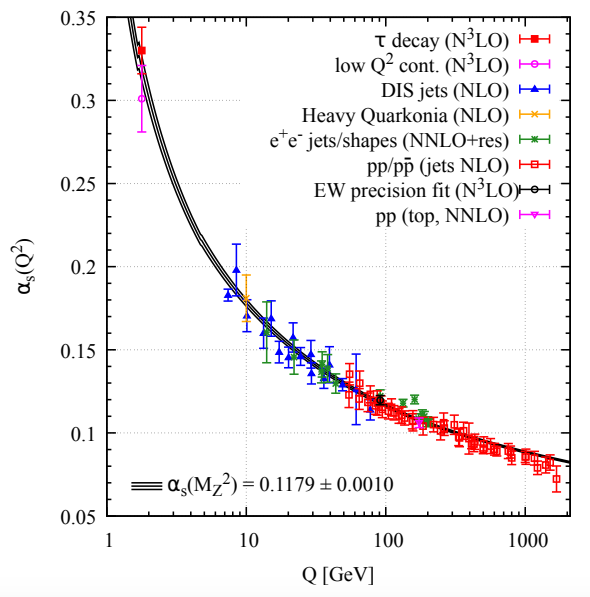
\includegraphics[width=0.50\textwidth]{Figures/Chapter1/QCDCoupling.png}
\caption{The running of the strong coupling constant $\alpha_s$ in different experiments at different energy scale $Q$ and the comparison with QCD calculations are shown above. Image from: \cite{AlphaTheoEx}}
\label{QCDCoupling}
\end{center}
\end{figure} 

An excellent agreement between theoretical predictions and experimental results of the strong coupling constant is observed in Figure~\ref{QCDCoupling}. 

\subsection{Perturbative QCD}

It is mathematically proven that there is in general no closed form expression for the partition function $Z[J(x)]$ Standard Model Lagrangian under the Quantum Field Theory framework.

\begin{equation}
Z[J(x)] = \int \mathcal{D}[\phi(x)] e^{iS + \int d^4 x J(x) \phi(x)}
\end{equation}

Therefore, physicists develop perturbation theory in Quantum Field Theory and apply it to the Standard Model. Physicist perform asymptotic expansions to obtain power series of the coupling constants and approximately calculate the expectation values of the observables to prediction experimental results.

For QCD, ,  perturbation theory is applicable to QCD in high energy and hard scattering processes since the coupling constant is much less than 1. Feynman rules and diagrams are applicable in the matrix element to evaluate the cross section of hard parton-parton scattering. Perturbative QCD (pQCD) calculations have been tested with various experiments such as electron-positron annihilations, deep inelastic electron-proton scatterings, and high energy proton-proton collisions.

\subsection{Non-perturbative QCD}

For soft scattering processes at low energy, the strong coupling constant is greater than 1. Perturbation theory of QCD breaks down. Many low-energy QCD processes such as hadronization and hadron-hadron interactions are non-perturbative. Historically, physicists developed Lattice gauge theory where the spacetime is discretized into lattice with finite size to evaluate the path integrals in the partition function $Z[J(x)]$. Lattice QCD can be applied to calculate the mass of the proton \cite{LQCDProtonMass}. Aside from Lattice gauge theory, effective theory is also to study non-perturbative QCD. For example, Chiral Perturbation Theory, where a low-energy effective Lagrangian in degree of freedom of hadrons is constructed by exploiting the approximate chiral symmetry while preserving other symmetries of parity and charge conjugation, has achieved some success to study pion-nucleon scattering \cite{ChiPT}. Non-perturbative QCD has achieved many successes in hadronic physics. Currently, some novel developments applying non-perturbative QCD to understand nuclear structure and nucleon spin structure are being carried by physicists. For instance, Chiral Perturbation Theory has been applied to study light nuclei structure such as ${}_{3}^{6}Li$ and ${}_{5}^{10}B$ \cite{ChiPTNuclear} and Lattice is employed to investigate nucleon spin structure \cite{LatticeNuclSpin}. 

\subsection{QCD Factorization Theorem}

The QCD factorization theorem states that in events with hadrons as incoming particle involving both hard and soft QCD processes, hard and soft process are mathematically factorized in the cross section computation shown schematically below \cite{QCDFactorization}: 

\begin{equation}
\sigma = PDF \otimes Diagrams \otimes FF
\end{equation}

\begin{figure}[hbtp]
\begin{center}
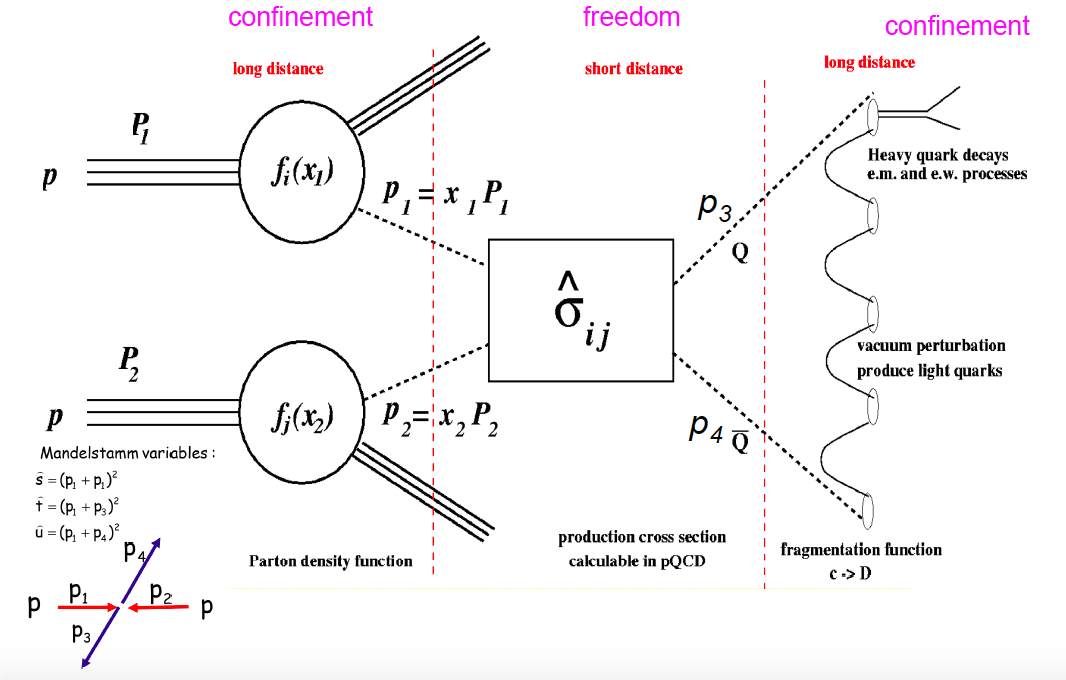
\includegraphics[width=0.75\textwidth]{Figures/Chapter1/QCDFactorizationTheorem.png}
\caption{The QCD factorization theorem applied to a pp collision event involving in soft and hard processes are shown above.}
\label{QCDFacTheo}
\end{center}
\end{figure} 

The hard processes are encoded in the factor of partonic cross sections while the soft processes are measured in experiments. Physicists employ parton distribution function (PDF), defined as the probability of finding a particle with a certain longitudinal momentum fraction $x$ at resolution scale of $\mu^2$, to describe the initial kinematic of partons inside hadrons \cite{PDFRef} and fragmentation function (FF), defined as the probability of a parton turn into a hadron $D_i^h(z)$ for a given energy fraction of the parton $z$ at resolution scale of $\mu^2$, to describe the hadronization process of partons \cite{QCDFFunc}. 

In addition to PDF, we could also define nuclear PDF (nPDF) for \cite{nPDF} to describe the parton kinematics inside nucleus. nPDF could be understood as the PDF of nucleons modified by the nuclear environment. Both parton distribution function and fragmentation function are extracted in experiments.

Physicists apply QCD factorization theorem to perform pQCD calculations and compare them with hadron spectra in electron-positron ($e^+e^-$), electron-proton ($ep$), and proton-proton ($pp$) collisions.

\subsection{Color Confinement}

Another feature of QCD as a non-abelian gauge theory is color confinement. The strong force carrier gluon itself is also color charged. Color charged partons, namely quarks and gluons, are never detected in isolation. In experiments, only color neutral hadrons are detected. Currently, the analytic explanation of color confinement is still not yet rigorously proven. The theoretical explanation of color confinement in QCD remains one of the unsolved problem in physics. 

\subsection{Hadronization}

The formation process hadrons from partons is called haronization. Because in experiments we can only measure final state hadrons, in order to study the interactions and dynamics of quarks and gluons during partonic stage from hadron spectra, we also need to understand hadronization mechanisms. However, hadronization is in general non-perturbative and cannot yet be described by first principle QCD calculations. Therefore, physicists make phenomenological models such as the Statistical Hadronization Model \cite{SHM}, Lund String Model \cite{LSM}, Cluster Hadronization Model \cite{CHM}, Quark Coalescence Model \cite{QCM} to study hadronization. Figure \ref{HadMech} schematically shows the hadronization of heavy quarks via fragmentation and recombination mechanism.

\begin{figure}[hbtp]
\begin{center}
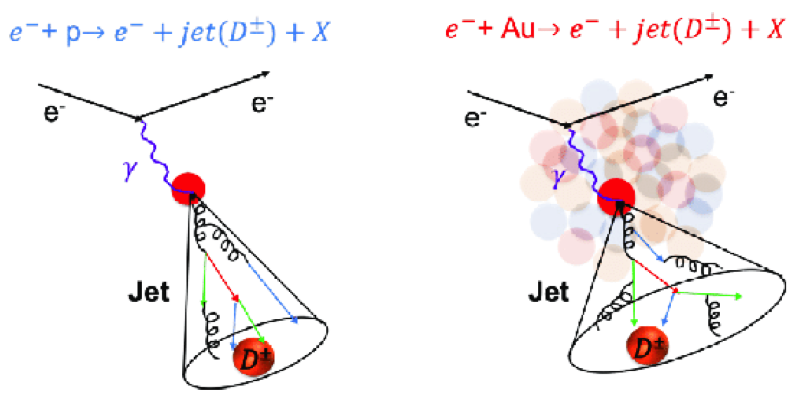
\includegraphics[width=0.48\textwidth]{Figures/Chapter1/FragCartoon.png}
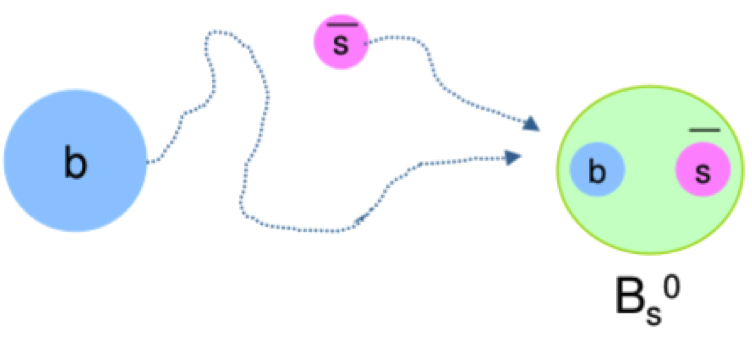
\includegraphics[width=0.48\textwidth]{Figures/Chapter1/CoalCartoon.png}
\caption{The fragmentation process of charms quarks hadronize into $D^\pm$ (left) and the coalescence process of beauty quark combining with a strange quark nearby to form a $B^0_s$ are shown above.}
\label{HadMech}
\end{center}
\end{figure} 


\subsection{Initial State and Final Effect}

In high energy proton-nucleus ($pA$) collisions, protons scatter off nucleons inside nuclei. Assuming QCD factorization still holds, nPDF could be applied to calculate the cross section of particle production. The initial state effects of nuclei including event-by-event geometry fluctuations due to nuclear dynamics \cite{GuntherV3}, nuclear shadowing effect \cite{IntroShadow}, EMC effect \cite{EMC} will modify the PDFs of nucleons in nuclei compare to PDFs of nucleons in vacuum. 

In the final state, the struck parton will lose energy from the interaction with the nuclear fragment and modify the final state hadron spectra. Because the parton-hadron interaction is generally non-perturbative, to retain the formula of QCD factorization theorem, the parton FF is modified \cite{CNEEFF}. These initial stage and final stage effects in $pA$ collision are call cold nuclear matter effects. 

\section{Hot QCD}

\iffalse 

\subsection{Initial State and Final Effect}


The development described in the previous section applies in small systems, for example, $e^+ e^-$, $ep$, and $pp$ collisions. In the smallest collision system $e^+e^-$, there is no initial state effect since the electron and positrons are point-like. In $ep$ and $pp$ collision, the initial state effects are encoded in the proton PDF. 

In high energy proton-nucleus collisions, proton scatter off nucleons inside nucleon. Assuming QCD factorization still applies, we can define nPDF to describe the kinematics of quarks inside nucleons of nucleus. We can see that there will be modification to the PDF for a nucleon vacuum due to the nucleon dynamics in the nuclei we can study the cold nuclear matter effect and probe the nPDF. In pA collisions, there many initial state effect depdendng on the collision $x$ and $Q^2$. For instance, we have nuclear shadowing, gluon saturation, and EMC effect. Both nPDF and the struck parton interact with the nuclear fragment will affect the final state hadron spectra. We call these effects in pA collision as cold nuclear matter effect.
%Hence, in addition to the initial state effect, there are also final state hot QCD matter effects in high energy nucleus-nucleus collisions.  

Initial state CGC 

\fi

\subsection{QCD in Finite Temperature} 

%In high energy, quarks and gluons inside nucleons of the nuclei become relevant to describe the event. As the energy increase, the quark and gluon density of the collision system increases. During the collisions, many quarks and gluons interact with each with in a small volume. 

In a system of dense and energetic quarks and gluons confined in a given size of volume, they scatter with each other and exchange momenta via the strong interaction. Many-body dynamics between quarks and gluons become relevant. In the limit of large number of quarks and gluons, after a sufficiently long period of time, the system eventually converges to the thermal equilibrium state via strong interaction \cite{MLBThermal,ADSCFTThermal,QCDThermal} regardless of its initial states. Therefore, a description based on thermodynamics can be formulated to study such systems \cite{QCDThemDyn}. We call this thermalized many-body system of quarks and gluons to be QCD matter. Therefore, a thermodynamic variable temperature ($\mathbf{T}$) can be introduced to characterize these many-body QCD systems. The study of many-body QCD in finite temperature is called hot QCD. 



\subsection{Temperature Dependence of QCD Static Potential}. 

If we consider two color charged quarks in the limit of infinite mass and are essentially at rest in the lab frame, we can define a QCD static potential between these two quarks due to the strong interaction. In vacuum, such a potential is called ``Cornell Potential'' \cite{Cornell}. The potential as a function of the distance between two quarks is shown as follows:

\begin{equation}
V(r) = -\frac{\alpha_{eff}}{r} + \sigma r
\end{equation}

Here, $\alpha_{eff}$ is the effective strong coupling coupling between the two quarks and $\sigma \simeq 0.184$ GeV/c is the string coupling constant \cite{CornellEquation}. 

Now if we consider a thermalized system in finite temperature $T$, the potential becomes: 

\begin{equation}
V(r) = -\frac{\alpha_{eff}}{r} e^{-m_D r} + \frac{\sigma}{m_D} (1 - e^{-m_D r})
\end{equation}

Here, $m_D \sim g_s T$ is the Debye mass due to Debye color screening effect \cite{CSEff}, which essentially modifies the gluon propagator by inserting a finite mass term: $-i \frac{g^{\mu\nu}}{q^2} \rightarrow -i \frac{g^{\mu\nu}}{q^2 - m_D^2}$. We have observed that as $V(\infty) = \frac{\sigma}{g_sT}$, which is finite for $T>$0. In fact, Equation (2) reduces to the Cornell potential when $T =$ 0. The QCD static potential is shown below in Figure~\ref{QCDPotential} \cite{TDepCornell}


\begin{figure}[hbtp]
\begin{center}
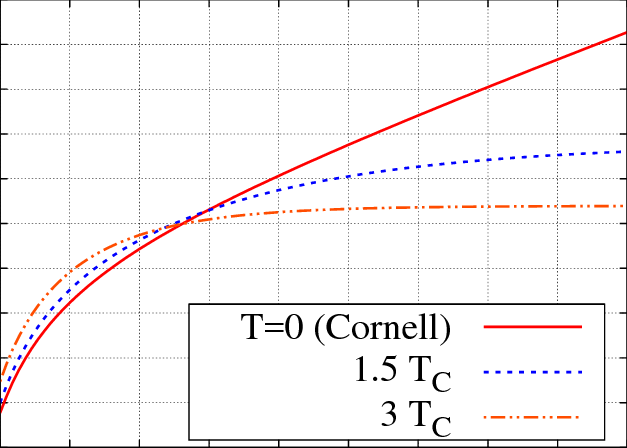
\includegraphics[width=0.55\textwidth]{Figures/Chapter1/QCDPotential.png}
\caption{The QCD potential $V(r)$ from at zero and at finite temperatures as a function of distance $r$ is shown above. Here, the critical temperature $T_c $ = 192 MeV. We can see that the QCD saturates at a finite value at finite temperature. }
\label{QCDPotential}
\end{center}
\end{figure} 


\subsection{Color Deconfinement}

As mentioned in the sections above, at finite temperature, the QCD static potential is screened and color degree of freedom become relevant in the system. As the temperature of the system increases, the quarks and gluon inside color-neutral hadrons will have more available space to move around and start to deconfine \cite{DeconfineTemp}. At some critical temperature $T_c$, quarks and gluons confined in hadrons will melt and form a new state of color deconfined QCD matter, which is called Quark-Gluon Plasma (QGP) \cite{QGPDeconfine}. The typical temperature of QGP is in the order of a few hundred MeV or about $10^{12}$ K, which is about hundreds of thousands times hotter than the core of the Sun. It is belived that QGP existed in the early universe several microsecond after the Big Bang \cite{}. Cosmologically, the study of QGP will help us understand the quark epoch and quark-hadron phase transition to under the history of the universe. 

%There are some interesting QCD phenomenologies involving temperature as listed in the following subsections.

%Hot applies in AA collision where a thermalized system is created. 

\subsection{QCD Phase Diagram}

Similar to form everyday matters such as metal, water, wood, glass, and plastic, which are formed by electromagnetic interaction and could all be described macroscopically by equations of states that are parameterized by thermodynamic variables. 
\iffalse Figure~\ref{QEDPhaseDiagram} shows the phase diagram of water ($\mathrm{H_2O}$) at different temperature and pressure:

\begin{figure}[hbtp]
\begin{center}
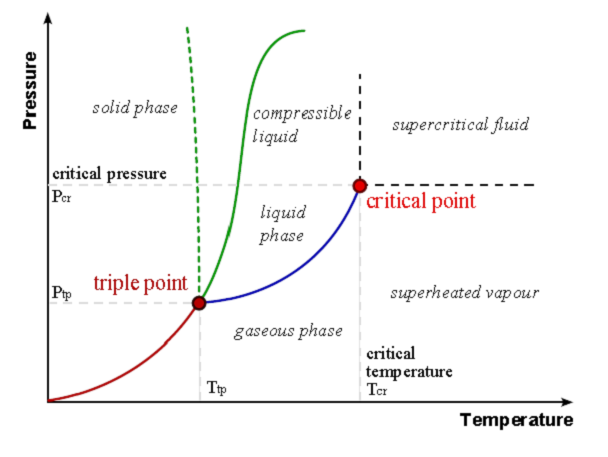
\includegraphics[width=0.45\textwidth]{Figures/Chapter1/WaterPhaseDiagram.png}
\caption{The P-T diagram of water in gas, liquid, solid phases is shown above.}
\label{QEDPhaseDiagram}
\end{center}
\end{figure} 

 
 \fi
Similarly, thermodynamical variables, for instance temperature ($\mathbf{T}$) and baryon chemical potential ($\mu_{B}$) can be introduced to characterize the equation of state of QCD matter formed via the strong interaction between many quarks and gluons. %Similarly, QCD matter is the matter formed by numerous quarks and gluons via the strong interaction and can also be describe by equations of states. L
Like our everyday matter which has gas, liquid, and solid phases at different pressure and temperature, QCD matter also has different phases at different temperature and baryon chemical potential. and can be describe by QCD phase diagrams. Figure~\ref{QCDPhaseDiagram} shows the QCD phase diagram at different temperature and baryon chemical potential:

\begin{figure}[hbtp]
\begin{center}
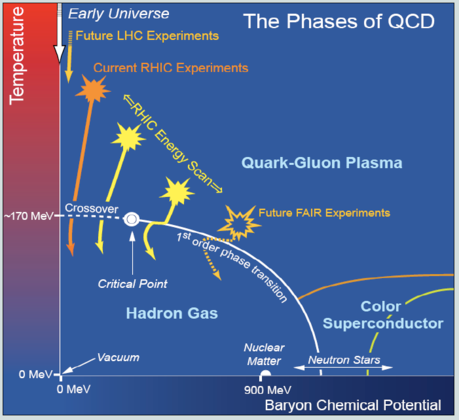
\includegraphics[width=0.60\textwidth]{Figures/Chapter1/QCDPhaseDiagram.png}
\caption{The theoretical QCD phase diagram of different QCD matter, including hadron resonance gas, quark-gluon plasma, neutron star, and color superconductor, as function of temperature and baryon chemical potential is shown above. The solid line indicates the conjecture of first order phase transition between quark-gluon plasma and hadron gas while the dash line is a smooth crossover. Thermodynamically, a critical points must exist in the boundary of smooth crossover and first order phase transition.}
\label{QCDPhaseDiagram}
\end{center}
\end{figure} 

We consider a system of free up and down quarks, antiquarks and gluons in temperature $T$ and baryon chemical potential $\mu_B$. According to MIT Bag Model \cite{MITBag}, its equation of state is given by

\begin{equation}
\epsilon(T,\mu_B) = \frac{37\pi^2}{30} T^4 + \frac{\mu_B^2}{3}T^2 + \frac{\mu_B^4}{54\pi^2} -  \mathcal{B}
\end{equation}

\iffalse
\begin{equation}
\epsilon(T,\mu_B) = \frac{37\pi^2}{30} T^4 + \frac{\mu_B^2}{7}T^2 + \frac{\mu_B^4}{161\pi^2} -  \mathcal{B}
\end{equation}
\fi

Here $p$ is the pressure and $\mathcal{B}$ is the bag constant, which can be understood as the pressure of the vacuum on the quarks and gluons to make them form hadrons with finite volume.

In a system of interacting quarks and gluons at $\mu_B=0$, based on lattice QCD calculations \cite{LatticeQGP}, the reduced energy density $\epsilon/T^4$ as a function of the temperature $T$ is shown below


\begin{figure}[hbtp]
\begin{center}
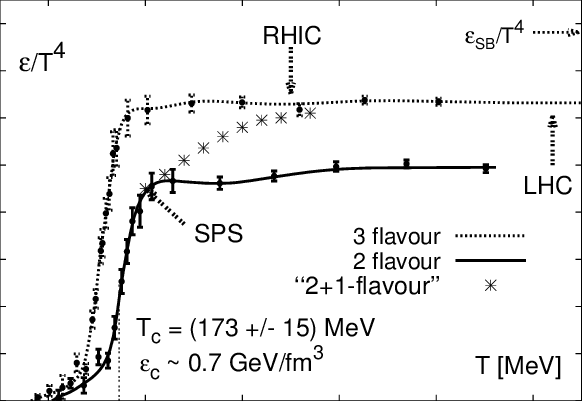
\includegraphics[width=0.60\textwidth]{Figures/Chapter1/LatticeData.png}
\caption{The reduced energy density $\epsilon/T^4$ as a function of temperature $T$ for different number of flavor scenarios from the lattice QCD calculations (data points) and the interpolation curves are shown above.}
\label{QCDPhaseDiagram}
\end{center}
\end{figure} 


A steep increase of the $\epsilon/T^4$ near the critical temperature at around $T_c  = 173$ MeV is observed, which signals the transition from hadron gas to the QGP \cite{PhaseTrans}. Experimentally, the critical point is estimated to be around $T_c = 175^{+1}_{-7}$ MeV and $\mu_B = (22 \pm 4.5)$ MeV \cite{CriticalPointEX} .






%Phase transition plot from LQCD

%Lattice QCD calculation has shown that.



%In the QCD phase diagram 

%Describe the diagram with QGP, Hadron Gas, and color superconductor.

%Talk a little about phase transition and critical point.

\section{High Energy Nuclear Physics}

Nuclear Physics is the study of atomic nuclei and their constituents and interactions. The typical energy scales of nuclear physics range from MeV to GeV. High Energy Nuclear Physics is a subfield of Nuclear Physics at an energy scale on the order of GeV. Its main goal is to under the physics of QCD matter from various approaches such as collider experiments, astrophysical observations, physics simulations, and theoretical modelings. In this thesis, I will focus on the research of QGP from the experimental approach using high energy heavy-ion colliders.

\subsection{Laboratories}

In laboratories, high energy nuclear physicists accelerate and collide heavy ions (A > 56) at center of mass high energy per nucleon at grater than 1 GeV to create extremely hot and dense conditions and study QGP. Relativistic heavy-ion collision is also known as ``The Little Bang'' compared to ``The Big Bang'' in cosmology \cite{LittleBang}. Historically, many colliders, such as the Alternating Gradient Synchrotron (AGS) at Brookhaven National Laboratory (BNL), in Upton, Long Island, New York and Super Proton Synchrotron (SPS) at European Center for Nuclear Research (CERN) in Meyrin, Switzerland, and GSI at Helmholtz Centre for Heavy Ion Research with both proton-proton and relativistic heavy-ion collision capabilities, have been built and established high-energy nuclear physics research programs. Today, two active colliders facilities, the Relativistic Heavy Ion Collider (RHIC) at BNL and the Large Hadron Collider (LHC) at CERN, are running at a wide range energies with various nuclei species and different impact parameters. In the future, another collider, called Facility for Antiproton and Ion Research (FAIR) running at relatively low energies, is being constructed at Darmstadt, Germany to map the location of the critical point in the QCD Phase Diagram. 

In addition to collider facilities, QGP might also be studied from astrophysical observations. For instance, strange stars, a quark star made of strange quark matter, may come from stable strangelet according to Bodmer--Witten conjecture \cite{SQMReview} or exist in the core of neutron stars under extreme pressure and temperature. It is believe there are several potential strange stars candidates according to telescope observations and gamma ray burst analysis \cite{SS1,SS2,SS3}.

%\subsection{Heavy-Ion Accelerators}

\subsection{Relativistic Heavy Ion Collider (RHIC)}

Located at BNL in Upton, Long Island, New York, United States of America, RHIC is one of the major high energy accelerator facilities and currently the highest energy collider in America. It is a circular collider with a circumference of 3.843 kilometers and can provide proton energy up to 500 GeV and gold ion energy up to 200 GeV \cite{RHICReport}. It was built in 2000 in order to search for a strongly interacting hot and dense state of nuclear matter created under ultra-relativistic heavy-ion collisions, currently known as QGP, with hints from the measurements at AGS and SPS. Moreover, RHIC provides physicists with a wide range of energies and a variety of ion species from proton to deuteron and cooper to uranium to create different sizes of systems at different temperature and baryon densities. In addition, taking the advantage of its highly polarization beam with high luminosity, RHIC has great machine capabilities for cold QCD physics. Figure \ref{RHIC} below shows a sky view of RHIC at BNL:


\begin{figure}[hbtp]
\begin{center}
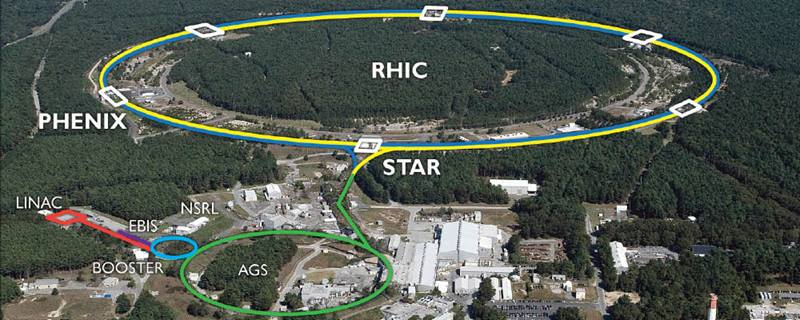
\includegraphics[width=0.85\textwidth]{Figures/Chapter1/RHIC.jpg}
\caption{The view of RHIC at BNL from the sky is shown above. The actual locations of other facilities at BNL, including Linac, Booster, EBIS, NSRL, AGS, and the experiments at RHIC such as, STAR and PHENIX, are also labelled.}
\label{RHIC}
\end{center}
\end{figure} 

Here is how RHIC accelerates charged particles to the energy scale of GeV per nucleon. For instance, if we consider the acceleration of a typical ion source gold (${}^{197}_{79}Au$) ion, we first use a cesium sputter ion source operated in the pulsed beam mode and point it to the gold metal to produce the $Au^-$ ion \cite{FirstAuSource}. Then, the $Au^{-}$ will undergo a series of electron stripping processes to reach the $Au^{79+}$ ion \cite{RHICStrpDetail}. First, 13 electrons are stripped by the carbon foil in the Terminal Stripping (S1) after the acceleration of tandem Van der Graaf generator to turn $Au^{-}$ into $Au^{12+}$. Then, the $Au^{12+}$ ion will go through the Object Foil (S2) at the second stripping stage and becomes $Au^{31+}$. Next, the $Au^{31+}$ will go through the third stripping station BTA foil (S3) made of aluminum and vitreous carbon between the Booster Synchrotron and AGS and becomes $Au^{77+}$. Finally, two more electrons of the gold ion $Au^{77+}$ are removed at the fourth stripping station ATF foil (S4) made of thin tungsten, located in between the AGS and RHIC. The fully stripped gold ions $Au^{79+}$ will then be injected to the blue and yellow rings at RHIC. For polarized protons, $H^-$ pass a single stripping stage called located in the Booster Synchrotron. The stripping station is called Linac-to-Booster (LTB) stripper made of carbon foils with special geometry and converts polarized $H^-$ to $H^+$. Figure \ref{AccAu} schematically shows the accelerating process of gold ions at RHIC \cite{AuStripRef}

\begin{figure}[hbtp]
\begin{center}
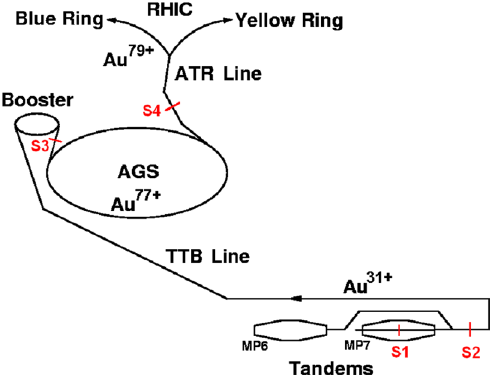
\includegraphics[width=0.45\textwidth]{Figures/Chapter1/AccAu.png}
\caption{The acceleration of gold ions for RHIC is shown above.}
\label{AccAu}
\end{center}
\end{figure} 

At RHIC, we will accelerate the $Au^{79+}$ ions in the superconducting Radio Frequency (RF) cavity under perpendicular electric and magnetic fields until they reach the energies up to about 100 GeV/c per nucleon. Subsequently, we collider them via bunch crossing at the interaction points of the experiments to perform relativistic heavy-ion collisions and study high energy nuclear physics. RHIC usually operates in the first six months of a calendar year. At RHIC, the energy can also be lower where the ion beam collides with ions at a lower energy in the laboratory frame. The STAR experiment at RHIC has already finished beam energy scan and is currently taking data in the fixed target program. 

%RHIC Versatile Machine - Energy + species 

\subsection{Large Hadron Collider (LHC)} 

Located at the border between Switzerland and France, LHC is one of the major high energy accelerator facilities in Europe and currently the highest energy collider in the world. It is a circular collider with a circumference of 26.7 kilometers and can provide proton energy up to 14.0 TeV and lead ion energy up to 5.02 TeV \cite{LHCReport}. It was built in 2008 with the main purpose to discover the Higgs Boson, perform precision measurements on SM, and search for Physics beyond SM. Due to its high energy ion capabilities, high energy nuclear physicists also use the existing general purpose detectors designed for high energy particle experiments at the LHC to conduct research on relativistic heavy-ion physics. LHC ion physics runs usually start at the end of the year and lasts for about a month. The photo taken from the sky to picture LHC is shown in Figure \ref{LHC}:

\begin{figure}[hbtp]
\begin{center}
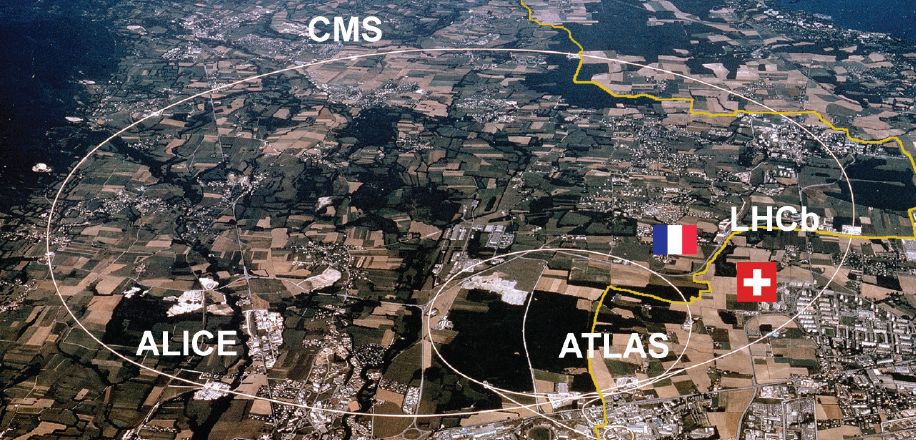
\includegraphics[width=0.85\textwidth]{Figures/Chapter1/LHC.png}
\caption{The sky view of LHC at CERN is shown above. The actual locations of the experiments at the LHC: ATLAS, CMS, ALICE and LHCb, as well as the French-Swiss border, are also displayed.}
\label{LHC}
\end{center}
\end{figure} 

CERN usually uses is lead ${}^{208}_{82} Pb$ ions, which are stable and approximately spherical. In the 2017 ion physics run, it also used the xenon ${}^{131}_{52} Xe$. Currently, there is also a discussion of potential future usage of lighter ions such as oxygen ${}^{32}_{16} O$ \cite{OORun}. Similar to RHIC, the lead ions at the LHC also undergo a series of stripping processes using stripping foils in to order to become partially ionized $Pb^{81+}$ \cite{LHCStrip}. Also, the lead ions pass a series of energy boosting before reaching to the desired energies at the LHC. Lead ions start from a source of vaporized lead and enter Linac 3 before being collected and accelerated in the Low Energy Ion Ring (LEIR) at the energy from 4.2 MeV to 72 MeV. Then, the lead ions will be injected to Proton Synchrotron (PS) to boost their energies. Next, they are sent to the Super Proton Synchrotron (SPS). Finally, the lead ions are injected to the LHC and increase their energies to TeV scale in two LHC rings with the RF cavity \cite{LHCReport}. Finally, the energetic lead ion beams from two LHC rings will collide with a small crossing angle at the interaction points of the LHC experiments. The CERN accelerator complex is shown schematically in \ref{CERNAccComplex} 


\begin{figure}[hbtp]
\begin{center}
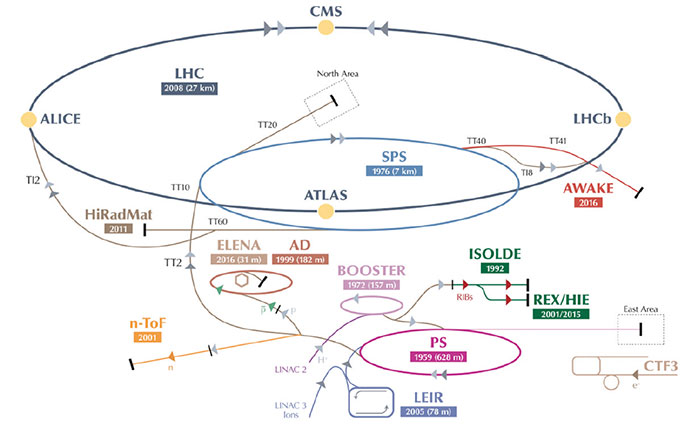
\includegraphics[width=0.65\textwidth]{Figures/Chapter1/CERNAccComplex.jpg}
\caption{The schematic overview of CERN accelerator complex with the accelerators labelled is shown above. Proton and lead ions are accelerated using these facilities and boost their energies to the TeV scale.}
\label{CERNAccComplex}
\end{center}
\end{figure} 

After Run III, LHC will upgrade to high-luminosity (HL) LHC and allows physicists to collect huge datasets, which is crucial to for precision measurements in heavy-ion physics program. Because the beam energy at the LHC is higher than RHIC, the QGP created at the LHC has a higher temperature and a smaller baryon chemical potential than the one created at RHIC.  

\subsection{High Energy Physics Coordinates}

As mentioned in the previous section, heavy-ion is in general highly relativistic. Therefore, Lorentz transformation will be relevant in our studies. In Cartesian coordinates $x^\mu = (t,x,y,z)$, under Lorentz transformation, if we boost the system by a speed $\beta$ in the $+z$ direction. The Lorentz gamma factor will be given by $\gamma = \frac{1}{\sqrt{1 - \beta^2}}$. The four vector $x^\mu \rightarrow x'^\mu$ transforms as follows

\begin{align}
   \begin{bmatrix} 
           t' \\
           x' \\
           y' \\
           z' \\
         \end{bmatrix} =
             \begin{bmatrix} 
             \gamma  & 0  & 0 & - \gamma \beta \\ 
            0 & 1 & 0 & 0 \\ 
             0 & 0 & 1 & 0 \\
             - \gamma  \beta & 0 & 0 &  \gamma \\
	\end{bmatrix} 
	  \begin{bmatrix} 
           t \\
           x \\
           y \\
           z \\
	\end{bmatrix}
\end{align}

The equation above is called the Lorentz Transformation. It is an orthogonal transformation preserving the Minkowski metric tensor $diag(1,-1,-1,-1)$ using particle physicists conventions.


Nowadays, heavy-ion detectors usually have $2\pi$ angular coverage in the transverse direction with some finite longitudinal acceptance along the beam line. They are essentially cylindrically symmetric. Hence, it is convenient and sensible to choose a cylindrical coordinate system and use Lorentz invariant kinematic variables. In general, we define the beam direction to be the z-direction of the coordinate system. Fort the standard cylindrical coordinates in the position space, the Lorentz four-vectors is $(t,x,y,z) \rightarrow (t, r, \phi, z)$. 


The relativistic coordinate system for our analysis is shown below in Figure \ref{HICoordinates}. 

\begin{figure}[hbtp]
\begin{center}
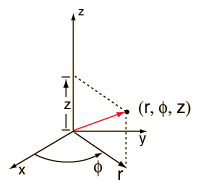
\includegraphics[width=0.40\textwidth]{Figures/Chapter1/PosCylindrical.png}
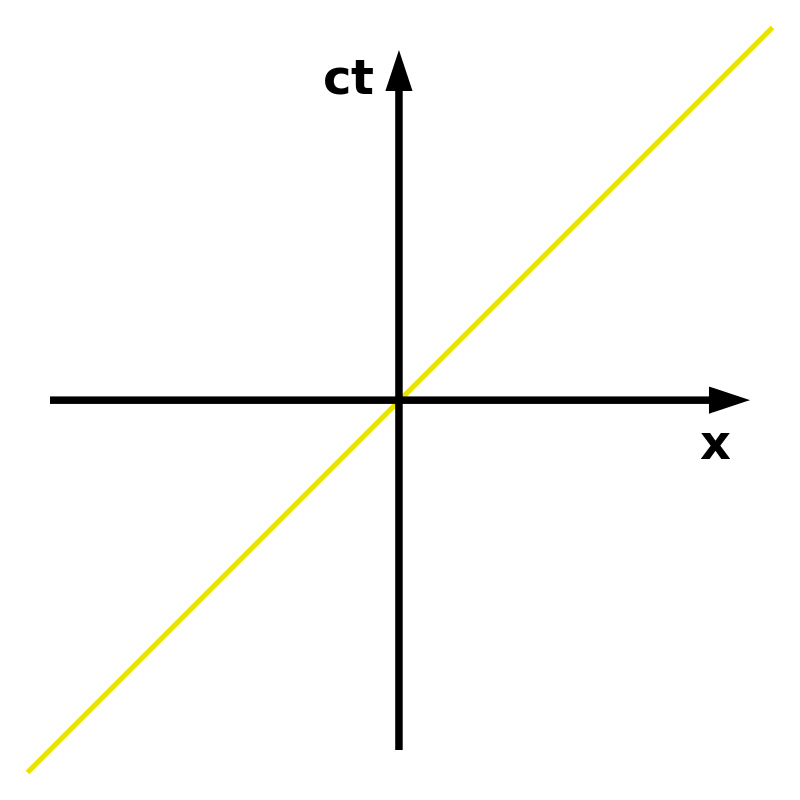
\includegraphics[width=0.40\textwidth]{Figures/Chapter1/STDiagram.png}
\caption{The cylindrical coordinate system in the position space (left) and the space time diagram (right) for relativistic heavy-ion physics analysis are shown above.}
\label{HICoordinates}
\end{center}
\end{figure} 


Thus, in the momentum space, we can use $p^\mu = (E,p_x, p_y, p_z) \rightarrow  (E,p_T, \phi, p_z)$ 

\begin{equation}
p_T = \sqrt{p_x^2 + p_y^2}
\end{equation}

\begin{equation}
\phi = \arctan(\frac{p_y}{p_x})
\end{equation}

We also define rapidity $y$, a relativistic version of velocity that can be convenient add to the boost.

\begin{equation}
y = \frac{1}{2} \ln \frac{E+p_z}{E-p_z}
\end{equation}


Experimentally, we also use pseudo-rapidity $\eta$, which is more directly connected to the detector measurements assuming ultra-relativistic limit kinematics ($E \rightarrow p$). The definition of pseudo-rapidity $\eta$ is shown as follows:

\begin{equation}
\eta =  - \ln \tan(\frac{\theta}{2})
\end{equation}

Here $\theta$ is the angle labelled in the left of Figure \ref{HICoordinates}. Particularly, $y = 0$ and $\eta = 0$ when $p_z = 0$. In addition, boosting by a speed $\beta$ in the longitudinal z-direction, we found that the rapidity simply shift by a const number $y' = y + \tanh \beta$. We should note that the cylindrical coordinates ($p_T$,$\phi$, $p_z$) are perfectly orthogonal while ($p_T$,$\phi$, $y$) or ($p_T$,$\phi$, $\eta$) are not.

For general collider experiments, two particles are moving toward each other with four-momenta $p_1^\mu$ and $p_2^\mu$ and interact with each other. It is also very convenient to use the Mandelstam variables $s, t, u$ in our studies. They are defined as follows

\begin{equation}
s \equiv (p_1 + p_2)^2
\end{equation}

\begin{equation}
t \equiv (p_1 - p_2)^2
\end{equation}

\begin{equation}
u \equiv (p_1 - p_3)^2
\end{equation}


In the center of mass frame, the momentum three vector follows $\vec{p_1} = -\vec{p_2} = \vec{p}$. Therefore, $p_1^\mu = (E, \vec{p})$ and $p_2^\mu = (E, -\vec{p})$. Hence, $s \equiv (p_1 + p_2)^2$ = $4E^2$ = $E_{CM}^2$. Hence, the center of mass energy of the collision system could be represented by the Mandelstam variable $\sqrt{s}$: $E_{CM} = \sqrt{s}$.


%\subsection{Heavy-ion Physics Detectors}

\subsection{Stages of Heavy-Ion Collisions}

In high energy heavy-ion collisions, both Electroweak and QCD processes occur in each event and contribute to the total cross section. We classify the events with elastic and inelastic reaction processes. For elastic processes, two nuclei scatter mainly electromagnetically with each via photon exchange without breaking themselves up or losing energy. For inelastic scattering, we classify diffractive and non-diffractive disassociation processes. In diffractive dissociation processes, the two nuclei may be slightly excited and lose a relatively small fraction of their energies, and produce relatively small number of particles. On the other hand, in non-diffractive dissociation processes, the nuclei lose a substantial fraction of their energies and produce a large number of particles \cite{CYWong}. 

Therefore, in events with significant contribution from non-diffractive dissociation, the interaction between two nuclei has multiple stages including both perturbative and non-pertubative QCD processes. We can define stages of heavy collisions and study the details of each stage. There are five stages: initial state of two highly Lorentz contracted nuclei before the collision, the very early pre-equilibrium stage when hard scatterings between partons inside nuclei begin, the rapid expansion of the fireball when the thermally and chemically equilibrated QGP is created, the hadronization stage after QGP expands and cools down, and the freeze-out stage when the inelastic scattering processes cease.


\begin{figure}[hbtp]
\begin{center}
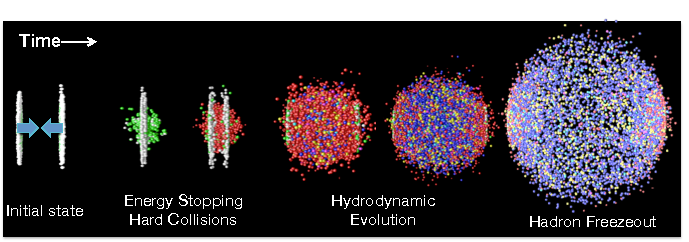
\includegraphics[width=0.80\textwidth]{Figures/Chapter1/Heavy-Ion-Process.png}
\caption{An event of a typical heavy-ion collisions event with different stages as time evolves is shown above.}
\label{HeavyIonStages}
\end{center}
\end{figure} 

\begin{figure}[hbtp]
\begin{center}
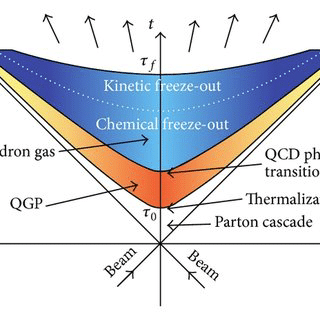
\includegraphics[width=0.45\textwidth]{Figures/Chapter1/HICSTEvolve.png}
\caption{The space-time evolution of heavy-ion collisions is shown above. It consists of four stages: initial state before the collision, early stage of hard scattering processes, the hydrodynamic expansion of QGP, hadronization after QGP expands and cools down, and the freeze-out stage, first chemical freezeout when the particle species no longer change, and finally kinetic freezeout when the elastic scattering processes ceas.}
\label{HICEvolution}
\end{center}
\end{figure} 

Theoretically, many phenomenological models such as Ultra-Relativistic Quantum Molecular Dynamics (UrQMD) and A Multi-Phase Transport Model (AMPT) are developed to describe relativistic heavy-ion collisions. 


\subsection{Global Event Observables}

Globally, we can define some physical quantities in heavy-ion collisions to generally characterize each event. Heavy-ion physicists define the impact parameter, centrality, number of participants, number of binary nucleon-nucleon collisions, and event multiplicity. We will discuss all of them below.

\textbf{Impact Parameter:} Prior to heavy-ion collisions, similar to other collider experiments, each event are prepared with the same unpolarized incoming particles with the same center of mass energy. Therefore, the incoming state $\ket{i}$ is used for each event. However, different from $e^+ e^-$ and $pp$ collision, in heavy-ion physics, we introduce another parameter called the impact parameter denoted $b$ to the transverse distance between center of two nuclei to classify the events. Therefore, the incoming state can be rewritten as  $\ket{i (b)}$. Figure \ref{IPHIColl} shows the definition of impact parameter in heavy-ion collision \cite{IPHICText}.

\begin{figure}[hbtp]
\begin{center}
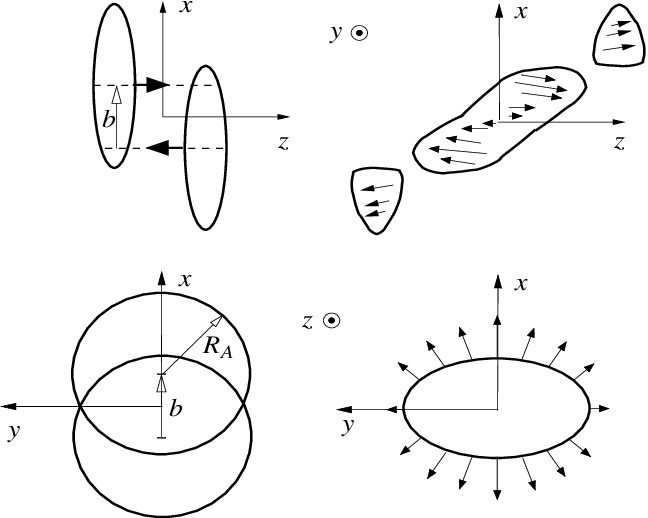
\includegraphics[width=0.60\textwidth]{Figures/Chapter1/IPHIColl.png}
\caption{The definition of impact parameter $b$ in heavy-ion collisions, the of overlapping interaction region, and the break up remnants of the two nuclei, which is called spectator, moving in the z-direction are shown above. An almond shape of the nuclear interaction region, which results in the azimuthal anisotropic emission of final state particles, is seen in heavy-ion collisions.}
\label{IPHIColl}
\end{center}
\end{figure} 


\textbf{Number of Participants:} Right at the end of heavy-ion collisions after two nuclei pass through each other, we can define the number of participants denoted $N_{part}$. The number of participants is essentially equivalent to the number of participating nucleons. The smaller the impact parameter, the more overlap volume between two nuclei, leading to a larger number of number of participating nucleons in the collision. The nuclear interaction system size is determined by the number of participating nucleons. However, due to event-by-event nuclei geometry fluctuations caused by the motion of nucleons inside nuclei \cite{GuntherV3}, it is more proper to say that the average number of participant $\langle N_{part} \rangle$ is related to the impact parameter.

\textbf{Number of Binary Nucleon-Nucleon Collisions:} In addition to $N_{part}$, we can also define another quantity that characterizes the detailed interaction in the events at rather hard scales. The number of binary nucleon-nucleon collisions, denoted $N_{coll}$, is also related to the impact parameter. At higher energy, nucleons inside nuclei become the relevant degree of freedom to describe the cross section. We could treat the collisions of two nuclei as the superposition of the collisions between nucleons inside the nuclei. Since binary nucleon-nucleon collision has a rather small cross section, it dominates the total nucleon-nucleon cross section according to binomial principle. Higher order effects, such as ternary nucleon-nucleon collisions, are negligible. The Glauber model \cite{CentPlot} is developed to study the relationship between $b$, $N_{part}$, and $N_{coll}$ in nuclei collisions and will be discussed in the following subsection.


\textbf{Centrality:} Experimentally, it is difficult to directly measure the impact parameter of each collision. Therefore, we define another physical quantity called centrality to characterize the impact parameter. The centrality ($C$) is defined as the fraction of the total nuclear interaction cross section: $C = \int^b_0 \frac{d\sigma}{dx} dx$ . Centrality is expressed in terms of percentage \cite{CentDef}. It is related to the quantity: $\frac{\pi b^2}{4\pi R_A^2}$ where $R_A$ is the radius of a nuclei defined above in Figure \ref{IPHIColl}. When the impact parameter between two nuclei is 0, the centrality is at 0\%. When the impact parameter between two nuclei is 2$R_A$, the centrality is 100\%. There is also a relationship between the centrality and the average number of participants. Heavy-ion experimental measurements are in general presented in terms of centrality or average number of participants. Experimentally, we look at the number of tracks and cluster energies of calorimeters at the forward direction, for instance, the forward hardonic calorimeters, to estimate the centrality \cite{ALICEZDC,CMSZDC,ATLASZDC}. 


\textbf{Virtuality:} Similar to deep inelastic scattering, we can also define the virtuality $Q^2$, which is the momentum transfer between the two nucleons in nucleon-nucleon collisions. To generate nucleon-nucleon collision event in Monte Carlo (MC) simulation, we used $\hat p_T$, defined as the transverse momentum of the hard subprocess, which is a quantity related to $Q^2$, developed by the high energy theory group of Lund University.


\textbf{Event Multiplicity:} We can also define the event multiplicity by counting the number of final state charged particles to quantify the activity of the event. Event multiplicity can be denoted as $N_{trk}$, number of tracks in the event, which is approximately proportional to the number of charged particle denoted as $N_{ch}$. Figure \ref{CentDefPlot} shows the correlation between the number of participants, their cross section, and the impact parameter in heavy-ion collisions, defining the centrality classes \cite{CentPlot}.


\begin{figure}[hbtp]
\begin{center}
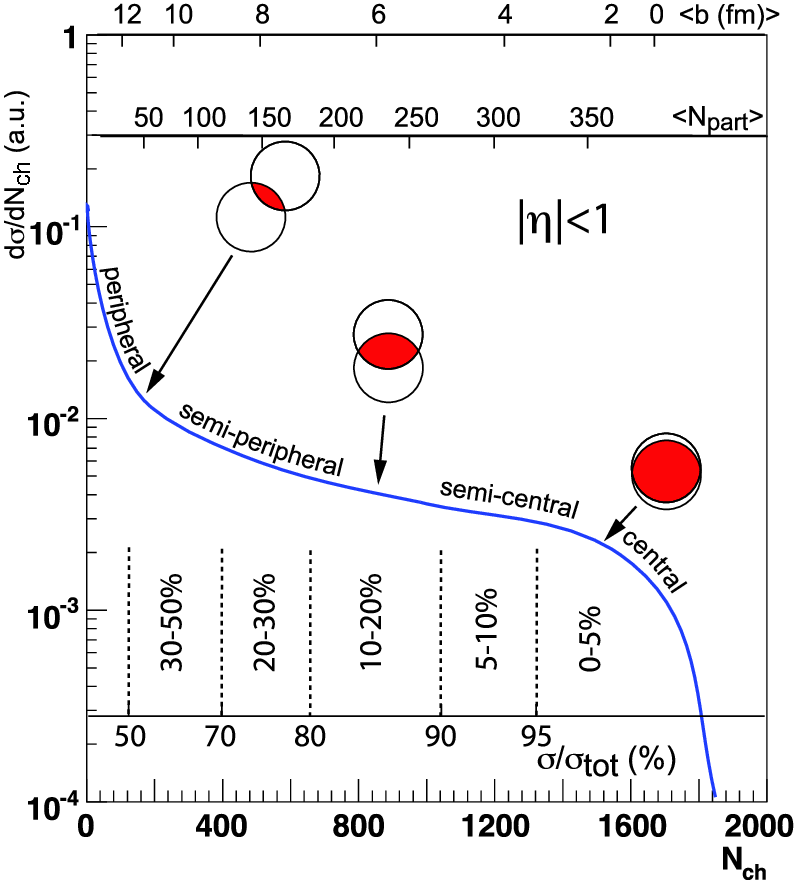
\includegraphics[width=0.55\textwidth]{Figures/Chapter1/CentDefPlot.png}
\caption{The plot showing relationship among number of charged particle, $N_{ch}$, related to the number of participants $N_{part}$, the differential cross section $\frac{d\sigma}{dN_{ch}}$, and the centrality, according to the Glauber Model calculations, is shown above.}
\label{CentDefPlot}
\end{center}
\end{figure} 


The initial global parameters such as the collisions energy, impact parameter, collision nuclei species, and polarization can be treated as knobs for high energy nuclear physicists to play with in order to study relativistic heavy-ion collisions and create strongly interacting systems with different sizes, chemical potentials, and temperatures in the QCD phase diagram. Figure \ref{STAREvtDisplay} shows an event display of thousands of tracks from a central Au + Au collision event at 200 GeV recorded by the Time Projection Chamber (TPC) of the STAR experiment at RHIC.


\begin{figure}[hbtp]
\begin{center}
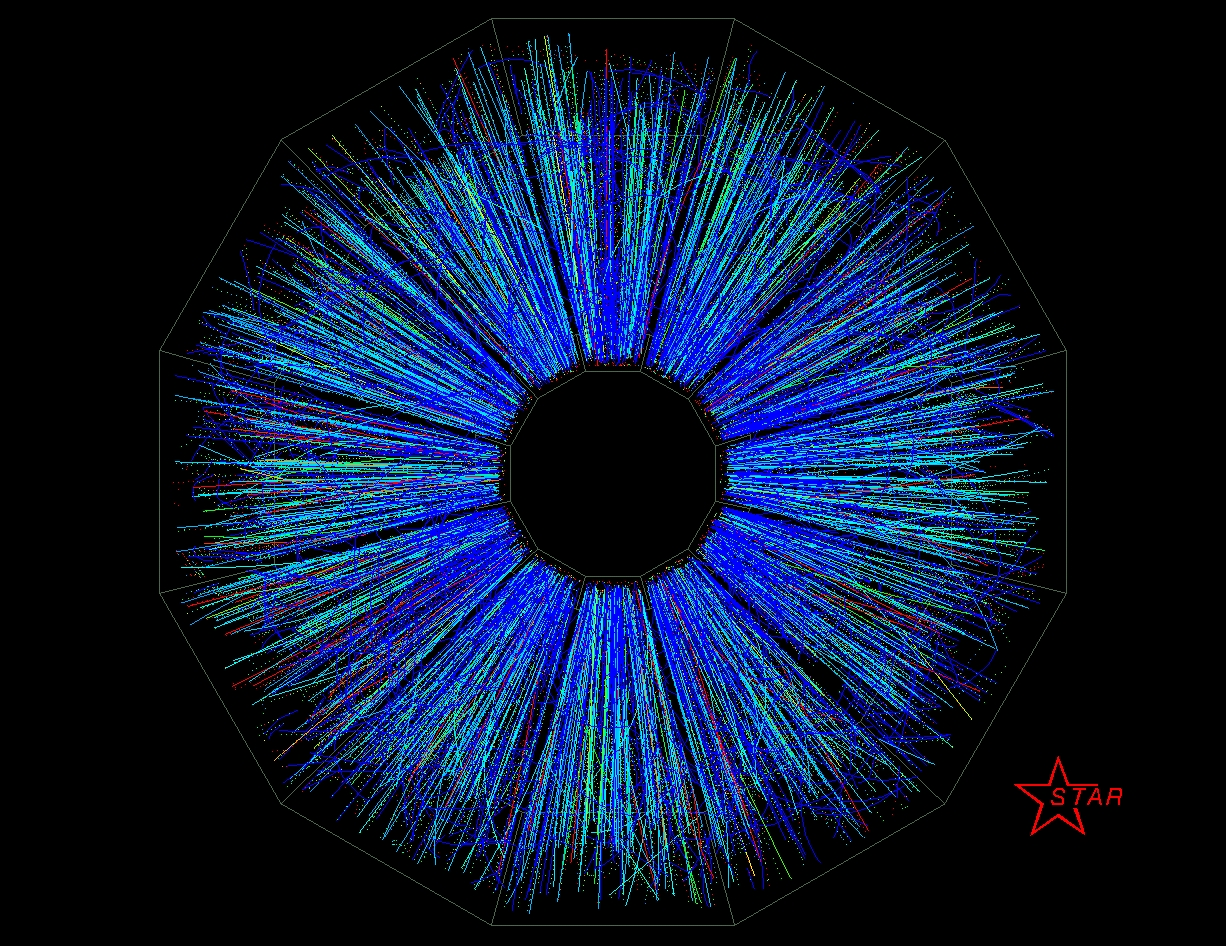
\includegraphics[width=0.50\textwidth]{Figures/Chapter1/STAREvtDisplay.png}
\caption{Two gold ions collide head-on in the STAR detector. The event with reconstructed tracks of final state particles are display by STAR TPC shown above. Image from \cite{STARTPC}}
\label{STAREvtDisplay}
\end{center}
\end{figure} 



\subsection{Glauber Model}

The Glauber Model, named after physicist Roy Glauber \cite{Glauber}, was originally developed to address high energy scattering problems with composite particles in the optical limit where optical theorem is applicable \cite{Optical1,Optical2}. It is a model describing two composite objects collider inelastically with each other and decompose the total cross section to the cross section of collision between two point objects. The Glauber Model can be applied to study nucleon-nucleus (N-A) and nucleus-nucleus (A-B) collisions with nucleon-nucleon (N-N) collisions and determine relationship between the global observables mentioned in the previous subsection.    

If we consider a spherically symmetric nucleus, the nuclear charge density can be described $\rho(r)$ by the Fermi distribution with three parameters below

\begin{equation}
\rho(r) = \rho_0 \frac{1 + w(r/R)^2}{1 + \exp({\frac{r-R}{a}})}
\end{equation}

The equation above is called the Wood-Saxon density formula. According to the Glauber Model \cite{Glauber}, the N-N inelastic cross section is denoted as $\sigma_{in}^{NN}$ and the effective thickness function of a nucleon is defined as a function of impact parameter in the transverse direction: $T(\vec{b})$. It is defined as follow

\begin{equation}
T(\vec{b}) =  \int \rho(\vec{b},z) dz 
\end{equation}

It is normalized to unity: $\int^{R_A}_0 T(\vec{b}) d^2b = 1$. $T(\vec{b})$ essentially depends on density of the nucleus $r(b)$. %If the nucleus is a uniform cylinder and the collide on its circular face along its height, then $T(\vec{b})$ will be a constant. 
Therefore, the probability that a nucleon collides with a nucleon inside the nucleus is given by $\sigma_{in} T(\vec{b})$. Therefore, the probability of $n$ nucleon collisions is given by

\begin{equation}
P_n = {A \choose n} \sigma_{in}^{NN} T(\vec{b})^{n} [1 - \sigma_{in} T(\vec{b})]^{A-n}
\end{equation}

Hence, if we consider a constant fraction of $\mu$ ($0 \le \mu \le 1$) of particle produced after each collisions, we can calculation the average event multiplicity $\langle N(\mu) \rangle$:

\begin{equation}
\langle N(\mu) \rangle = \Sigma_n P_n \Sigma^{n-1}_0 \mu^m =  \Sigma_{n-1} P_n \frac{1 - \mu^n}{1 - \mu} = \frac{1}{1-\mu} \{ 1 - [1 - (1-\mu) \sigma_{in} T(\vec{b})]^A \}
\end{equation}

It turns out that we have the following relationship between $N_{part}$ and $N_{coll}$ with $\langle  N(\mu) \rangle$  \cite{Glauber}

\begin{equation}
N_{part} = \langle N(\mu = 0) \rangle 
\end{equation}

\begin{equation}
N_{coll} = \frac{1}{2} \langle N(\mu = 1) \rangle = A T(\vec{b}) \sigma_{in}^{NN}
\end{equation}

In a more generalized case: A-B collisions, Figure \ref{GlauberRef} shows side view and beam-line view of heavy-ion collision of projectile B on target A


\begin{figure}[hbtp]
\begin{center}
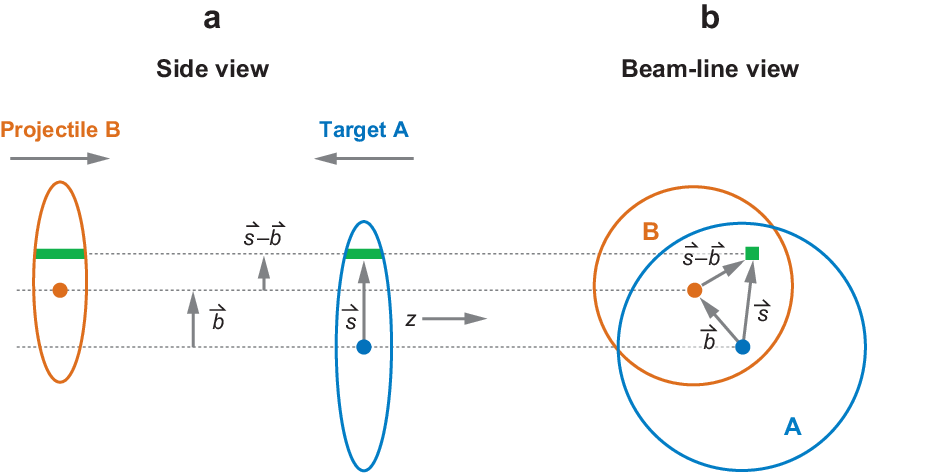
\includegraphics[width=0.65\textwidth]{Figures/Chapter1/GlauDefColl.png}
\caption{The A-B collision with the definition of the impact parameter vector $\vec{b}$ and the distance of nucleon to the center of projectile B $\vec{s}$ are shown above. The distance of the nucleon in B to center of the target A is $\vec{s}-\vec{b}$ according to vector subtraction rule. Here we assume both nuclei A and B are perfect spheres.}
\label{GlauberRef}
\end{center}
\end{figure} 

Using similar ideas \cite{CentPlot}, we could first calculate the effective thickness function $T_{AB}$ as follows:


\begin{equation}
T_{AB}(\vec{b}) = \int T_A(\vec{s}) T_B(\vec{b} - \vec{s}) d^2s 
\end{equation}



Now replacing T($\vec{b}$) in N-A by $T_{AB}(\vec{b})$ in A-B, we can obtain

\begin{equation}
\langle N(\mu) \rangle = \frac{A}{1-\mu} \int_0^b T_A(\vec{s}) \{1 - [1 - (1 - \mu) T_{B}(\vec{b}-\vec{s}) \sigma_{in}^{NN}]\}^A d^2s  +  \frac{B}{1-\mu} \int_0^b T_B(\vec{s}) \{1 - [1 - (1 - \mu) T_{A}(\vec{b}-\vec{s}) \sigma_{in}^{NN}]\}^B d^2s
\end{equation}


To obtain $N_{part}$, evaluate at $\mu = 0$, we get 

\begin{equation}
N_{part} =  A \int_0^b T_A(\vec{s}) \{1 - [1 - T_{B}(\vec{b}-\vec{s}) \sigma_{in}^{NN}]^A\}d^2s +  B \int_0^b T_B(\vec{s}) \{1 - [1 - T_{A}(\vec{b}-\vec{s}) \sigma_{in}^{NN}]^B\} d^2s
\end{equation}

To obtain $N_{coll}$, evaluate at $\mu = 1$, we get

\begin{equation}
N_{coll} = AB T_{AB}(\vec{b}) \sigma_{in}^{NN}
\end{equation}

In a very special case, assume the nuclei are simply perfect rigid sphere with the same radius and collide with zero impact parameter is $b=0$. That is $T_{A} \sigma_{in}^{NN} = T_{B} \sigma_{in}^{NN} = T_{AB} \sigma_{in}^{NN} = 1$, we get 


\begin{equation}
N_{part} = A + B
\end{equation}

\begin{equation}
N_{coll} = AB
\end{equation}

The results above of $N_{part}$ and $N_{coll}$ agree to our expectation. 

The comparison of the Glauber Model with simulations of the $N_{part}$ and $N_{coll}$ as a function of impact parameter $b$ is shown on Figure \ref{NPartandNColl} from the \cite{CentPlot}

\begin{figure}[hbtp]
\begin{center}
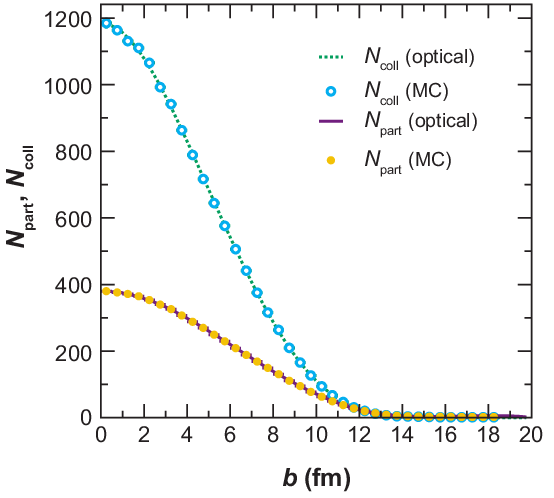
\includegraphics[width=0.50\textwidth]{Figures/Chapter1/NPartandNColl.png}
\caption{The $N_{part}$ and $N_{coll}$ as a function impact parameter calculated from the Glauber Model with optical approximation (lines) and from MC simulations (circles) are shown above. We can see they have almost perfect agreement with each other.}
\label{NPartandNColl}
\end{center}
\end{figure} 


Therefore, we can apply the Glauber model to determine $N_{part}$ and $N_{coll}$ for a given centrality range of AA collision ($T_{AB} \rightarrow T_{AA}$), which will be used in our analysis to obtain the corrected yield. It has been reported that the production of light hadrons, such as pions and kaons, are scaled as $N_{part}$ \cite{NPartScaling} while electroweak bosons, such as W and Z boson, are scaled as $N_{coll}$ \cite{NCollScaling}.

\section{Characterization of Quark-Gluon Plasma}

Equipped with the knowledge and collider technologies of heavy-ion collisions, we are ready to apply them to conduct scientific research on QGP in laboratories. The following subsections will describe the characterization of QGP from its predicted signatures to open questions today, which leads to my thesis research.

\subsection{Signatures}

QGP has been hypothesize long before its discovery as a color deconfined phase of quark matter named ``quark gluon plasma'' \cite{LeonQGP} and will demonstrate some specific benchmarks in experiments to prove the creation of QGP \cite{QGPSignature}. Here, four classic signatures of QGP will be discussed: $J/\psi$ and $\Upsilon$ suppression, jet quenching, elliptic flow, strangeness enhancement.  

\subsection{$J/\psi$ and $\Upsilon$ suppression} 

$J/\psi$ meson, as a type of heavy quarkonia, is bound state of $c\bar c$, made of charm quark and an anti-charm quark, with mass heavier than the $\Lambda_{QCD}$. Therefore, we could approximately treat the interaction between charm and the anti-charm quark with a static the Cornell potential $V(r)$ in the non-relativistic quantum mechanical hamiltonian system \cite{QuarkoniaV}: 

\begin{equation}
\hat H = \hat T + \hat V
\end{equation}

\begin{equation}
\hat H \ket{\psi} = i \frac{\partial}{\partial t}  \ket{\psi} 
\end{equation}

and solve Schrodinger equation the to describe $J/\psi$ mesons in vacuum. As we have seen in Section 1.3.2, with the QGP medium, at a finite temperature $T$, the potential is modified due to color screening effect. The distance between two charm quarks $V(r) \rightarrow \frac{\sigma}{m_D}$, which does not diverge, as $r \rightarrow \infty$. Therefore, the $c \bar c$ system could be unbounded if they have sufficiently high energy. In the field theory picture, this could be understood as the color string breaking between charm and anti-charm quark \cite{CSBQQ}, also known as quarkonia melting \cite{QQMelt}. Hence, with the influence of QGP at $T > 0$, the production cross section of $J/\psi$ will decrease compared to the vacuum at $T=0$. Experimentally, we define an observable to quantify the modification of particle production cross section in $AA$ collision compared to the reference $pp$ collisions normalized by the number of binary nucleon-nucleon collisions $N_{coll}$, which is defined in the previous subsection. We called this observable as nuclear modification factor denoted $R_{AA}$. Mathematically, $R_{AA}$ is defined as follows:

\begin{equation}
R_{AA} =\frac{1}{N_{coll}} \frac{\frac{d^2N_{AA}}{dp_T dy}}{\frac{d^2N_{pp}}{dp_T dy}} = \frac{1}{T_{AA}} \frac{\frac{d^2N_{AA}}{dp_T dy}}{\frac{d^2\sigma_{pp}}{dp_T dy}}
\end{equation}

Therefore, $R_{AA} < 1$ means suppression. $R_{AA} =1$ means no modification. $R_{AA} > 1$ means enhancement. Hence, in experiments, we expect to observe the $R_{AA} < 1$ a suppression of $J/\psi$ production. Figure \ref{JPsiSupp} shows the measurement of fully reconstructed $J/\psi$ at RHIC and LHC \cite{STARJpsi}


\begin{figure}[hbtp]
\begin{center}
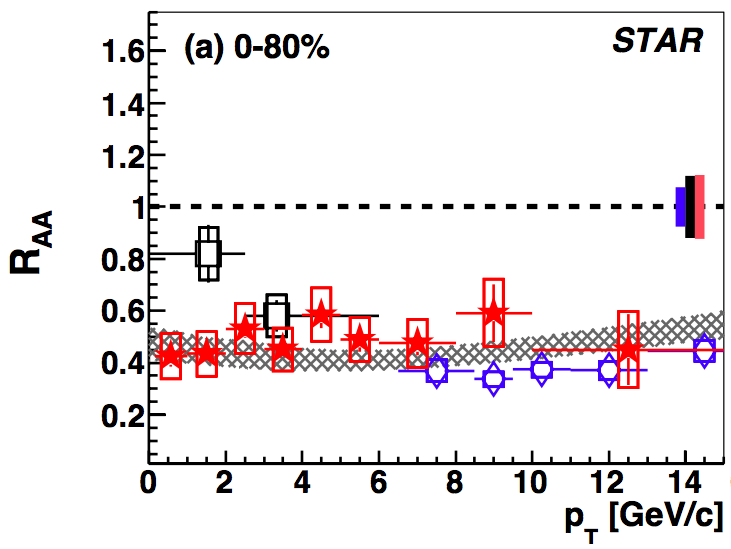
\includegraphics[width=0.47\textwidth]{Figures/Chapter1/STARPt.png}
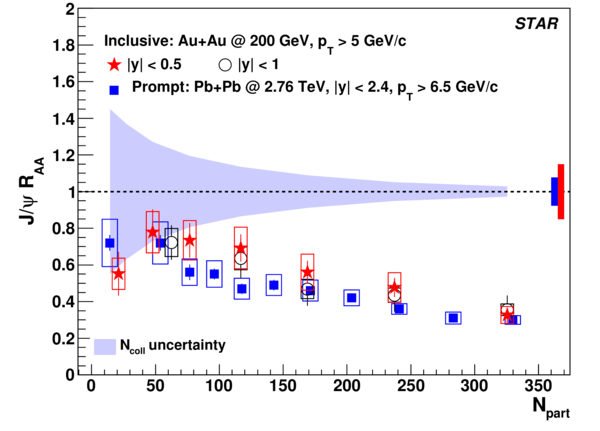
\includegraphics[width=0.487\textwidth]{Figures/Chapter1/STARNPart.png}
\caption{The nuclear modifications factor $R_{AA}$ of fully reconstructed $J/\psi$ as a function of $p_{T}$ (left) and $N_{part}$ (right) measured by the STAR experiment (red data points) at RHIC and CMS (blue diamond data points) and the ALICE (blue circle data points) experiment at the LHC are shown above. We can see that the $J/\psi$ $R_{AA}$ is below 1 for both $p_T$ and $N_{part}$. There is no significant $p_T$ dependence of $J/\psi$ $R_{AA}$. The $J/\psi$ $R_{AA}$ decreases as $N_{part}$ increases, consistent to the increasing creation probability of QGP with larger $N_{part}$.}
\label{JPsiSupp}
\end{center}
\end{figure} 

In fact, we could see that $R_{AA} < 1$ for every data point, which indicates a clear suppression of $J/\psi$ production from experiments at both RHIC and the LHC. However, we should note that the larger $J/\psi$ $R_{AA}$ observed at the LHC compared to RHIC could be explained by regeneration mechanism \cite{JPsiRegen}. %The observation of $J/\psi$ suppression is one of the earliest evidence of the discovery of QGP.

Similarly, we expect to see this in $\Upsilon$, which is made of $b \bar b$. Indeed, they expect to have sequential suppression since 3 $\Upsilon$ states: $\Upsilon(1S)$,  $\Upsilon(2S)$, and $\Upsilon(3S)$, could be observed in experiments. Because the total energy of the $b \bar b$ system or equivalently the rest mass: $m_{\Upsilon(3S)} > m_{\Upsilon(2S)} > m_{\Upsilon(3S)}$, a sequential suppression: $R_{AA}^{\Upsilon(1S)} > R_{AA}^{\Upsilon(2S)} > R_{AA}^{\Upsilon(3S)}$ should be observed if QGP is created. Figure \ref{UpsilonSupp} shows the measurements of fully reconstructed $\Upsilon$ states at RHIC and LHC \cite{STARUpsilonRef,CMSUpsilonRef}

\begin{figure}[hbtp]
\begin{center}
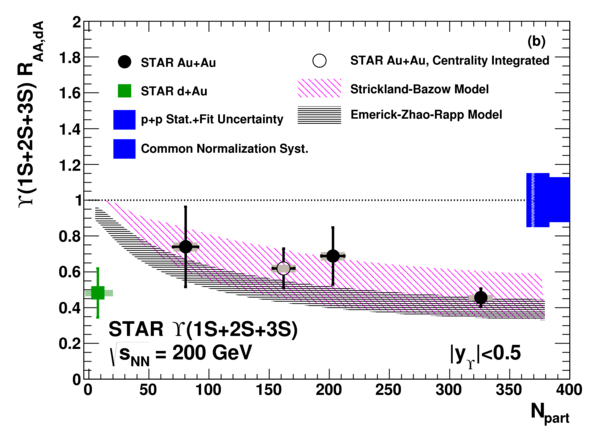
\includegraphics[width=0.52\textwidth]{Figures/Chapter1/STARUpsilon.png}
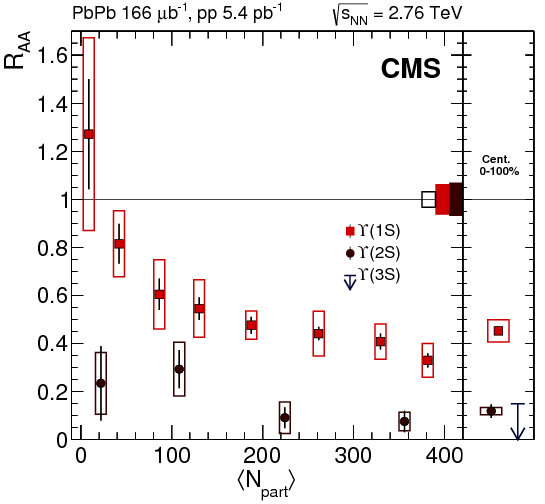
\includegraphics[width=0.40\textwidth]{Figures/Chapter1/CMSUpsilon.png}
\caption{The nuclear modifications factor $R_{AA}$ of fully reconstructed $\Upsilon$ as a function of $N_{part}$ measured by the STAR experiment (left) at RHIC and CMS experiment (right) at the LHC are shown above. We can see that the $R_{AA}$ of the three $\Upsilon$ states are below 1 when $N_{part} > 3$. The $\Upsilon$ $R_{AA}$ decreases as $N_{part}$ increases, consistent to the increasing creation probability of QGP with larger $N_{part}$. In addition, a sequential suppression of $\Upsilon$ $R_{AA}$ is observed by the CMS experiment: $R_{AA}^{\Upsilon(1S)} > R_{AA}^{\Upsilon(2S)} > R_{AA}^{\Upsilon(3S)}$, which agrees with the expectation QGP color screening effect.}
\label{UpsilonSupp}
\end{center}
\end{figure} 


\subsection{Jet Quenching} 

Experimentally, due to color confinement, it is impossible to directly detect and track the energetic partons. Therefore, physicists define jet as a spray of collimated hadrons within a narrow cone initiated from color charged partons. In nuclear and particle physics, jets are used to study the dynamics of partons before hadronization \cite{HERAJET} and understand the properties of QGP. A schematic view of a di-jet production from di-qurark event in electron-positron collider $e^+e^-\rightarrow q \bar q$ is shown below in Figure \ref{dijet}


\begin{figure}[hbtp]
\begin{center}
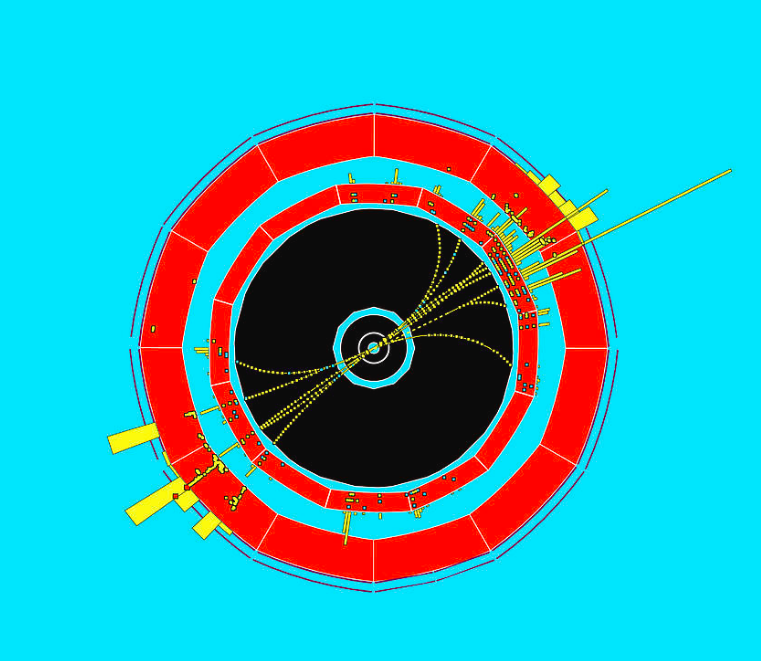
\includegraphics[width=0.50\textwidth]{Figures/Chapter1/DijetEvt.png}
\caption{The schematic display of a di-jet event from the ALEPH (a particle detector at the Large Electron-Positron collider) Experiment at the Large Electron-Positron Collider (LEP) is shown above. We can see two sprays of back to back particles within narrow cone, representing a di-jet event.}
\label{dijet}
\end{center}
\end{figure} 


Since we know QGP a color deconfined state of matter, an energetic parton carrying color charge traveling through the QGP medium is expected to lose a substantial a mount its energy to the medium. This is similar the effect that an electron beam losing energy in the electron-ion plasma via electromagnetic interaction \cite{ELossPlasma}. We call this effect as jet quenching. Figure \ref{JetELoss} shows jet quenching in QGP in AA collisions compared to pp collisions

\begin{figure}[hbtp]
\begin{center}
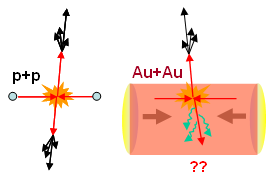
\includegraphics[width=0.45\textwidth]{Figures/Chapter1/JetELoss.png}
\caption{The schematic picture explaining jet quenching is shown above. Hard scatterings in pp collisions produce back-to-back "jets" of particles, but in Au + Au collisions, the presence QGP modifies the jets' properties.}
\label{JetELoss}
\end{center}
\end{figure} 


Experimentally, compared to pp collision where the QGP is not expected to be created, the jet spectra is modified by the QGP medium. The angular distributions would be broaden due to interaction with the medium. The $p_T$ spectra will be shifted to the left due to energy loss. This can be quantified by jet nuclear modification factor $R_{AA}$ similar to the $R_AA$ for quarkonium suppression mentioned previously. Figure \ref{JetRAA} shows the hadron angular correlation with the STAR experiment at RHIC and jet $R_{AA}$ as a function of $p_T$ with the ALICE experiments at LHC \cite{STARJetRef,ALICEJetRef}:
  
\begin{figure}[hbtp]
\begin{center}
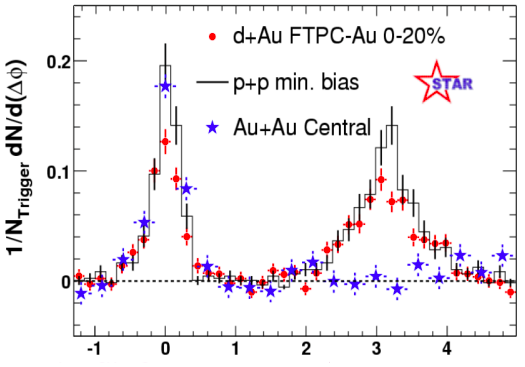
\includegraphics[width=0.55\textwidth]{Figures/Chapter1/HadronAngularSTAR.png}
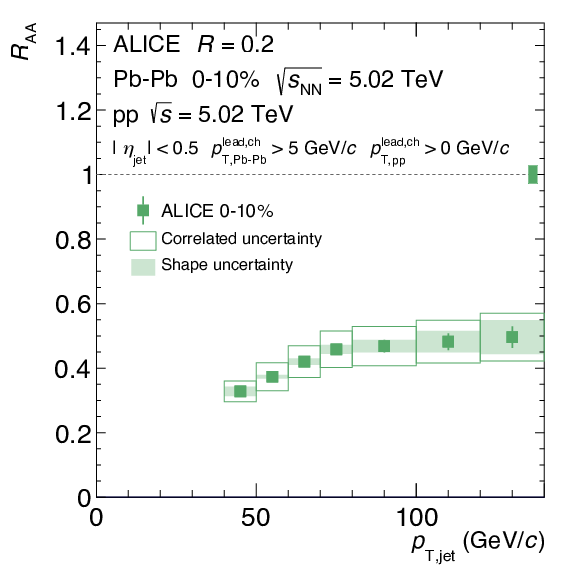
\includegraphics[width=0.40\textwidth]{Figures/Chapter1/JetRAAALICE.png}
\caption{The comparison of two-particle azimuthal distributions for central d + Au collisions to those seen in $pp$ and central Au + Au collisions measured with the STAR experiment and the jet $R_{AA}$ as a function $p_T$ measured by the ALICE experiment at LHC (right). From the STAR result, in central Au + Au collisions, the back-to-back peak has disappeared due to the redistribution of jet energy to the slow expanding medium constituents. The jet $R_{AA}$ from ALICE measurement is clearly below 1, suggesting that jets lose significant fractions of energy in $AA$ collision compared to $pp$.}
\label{JetRAA}
\end{center}
\end{figure} 

The jet $R_{AA}$ are all below 1 at RHIC and LHC \cite{ALICEJetRef,CMSJetSub}, which suggest jet quenching in AA collisions, supporting existence of QGP.

\subsection{Elliptic Flow} 

The reaction region in heavy-ion collisions, where the two nuclei overlap with each other, has an almond shape, which is azimuthally asymmetric. If a color deconfined matter QGP is created, particles emitted from the almond shape fire ball are expected to be anisotropic due to differences of the pressure gradient of the QGP in the and their path length through QGP in the x and y direction. Experimentally, physicists Dr. Arthur Poskanzer who sadly just passed away in June 30 2021, and Dr. Sergey Voloshin developed the event plane method to analyze the azimuthal anisotropy of particle emission in heavy-ion collisions \cite{EllipticFlow}. The reaction plane is defined as the plane of the impact parameter and the x-axis. Figure \ref{EventPlane} schematically shows the definition of reaction plane in heavy-ion collisions.

\begin{figure}[hbtp]
\begin{center}
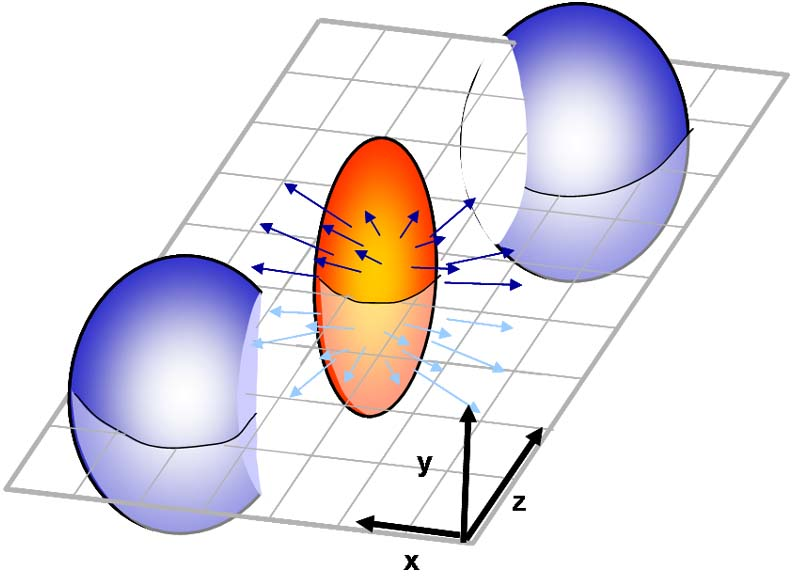
\includegraphics[width=0.40\textwidth]{Figures/Chapter1/ReactionPlane.jpg}
\caption{The figure above shows the ellipsoid of the overlapping nuclear reaction region of two nuclei in heavy-ion collisions. The reaction plane, which is the x-z plane shown as above, is constructed by the beam direction and the impact parameter vector. The emissions of particles are azimuthally anisotropic in the x-y plane.}
\label{EventPlane}
\end{center}
\end{figure} 

The particle spectra in heavy-ion collisions can be factorized as 

\begin{equation}
E \frac{d^3N}{d^3p} = E \frac{1}{2 \pi p_T}\frac{d^3N}{dp_T dy d\phi} = E \frac{1}{2 \pi p_T} \frac{d^2N_1}{dp_T dy} \frac{dN_2}{d\phi}
\end{equation}

Since the particle emission is azimuthally anisotropic, we can expand the $F(p_T,\phi,y) = \frac{dN_2}{d\phi}$ into a Fourier series \cite{EllipticFlow}:


\begin{equation}
F(p_T,\phi,y) = \frac{x_0(p_T,y)}{2\pi}  + \sum_{n=1}^{\infty}[x_n(p_T,y)\cos(n\phi)+y_n(p_T,y)\sin(n\phi)] 
\end{equation}

According to trigonometry, we get

\begin{equation}
F(p_T,\phi,y)  = \frac{x_0(p_T,y)}{2\pi} + \sum_{n=1}^{\infty}2v_n(p_T,y)\cos[n(\phi - \Psi_{n})]
\end{equation}

Here, $v_n = \frac{1}{2} \sqrt{x_n^2 + y_n^2}$ and $\Psi_{n} =\frac{1}{n} \arctan(\frac{y_n}{x_n})$. 

To find the Fourier coefficients $v_n$, we can apply the Fourier tricks to find $x_n$ and $y_n$.


Theoretically, because the function $\frac{dN_2(\phi)}{d\phi}$ is continuously analytical, we can use integral to find the Fourier coefficients [18] 
\begin{equation}
x_n =2\int_{0}^{2\pi} \frac{dN_2(\phi)}{d\phi}\cos(n\phi)d\phi 
\end{equation}
\begin{equation}
y_n =2\int_{0}^{2\pi} \frac{dN_2(\phi)}{d\phi}\sin(n\phi)d\phi 
\end{equation}

Experimentally, because our data take on discrete values, we can convert the integral into a sum 
\begin{equation}
x_n =\frac{2}{N}\sum_{n=1}^{N} \cos(n\phi)d\phi = 2\langle \cos n\phi \rangle
\end{equation}
\begin{equation}
y_n =\frac{2}{N}\sum_{n=1}^{N} \sin(n\phi)d\phi = 2\langle \sin n\phi \rangle
\end{equation}

Here, we sum up all tracks in the experiment to get the $x_n$ and $y_n$. Then, we will be able to find 

\begin{equation}
v_n = \frac{1}{2} \sqrt{x_n^2 + y_n^2} = \sqrt{(\langle \cos n\phi \rangle)^2+(\langle \sin n\phi \rangle)^2}. 
\end{equation}




In heavy-ion physics, the first order Fourier coefficient $v_1$ is called the directed flow. 

\begin{equation}
v_1 =  \sqrt{(\langle \cos \phi \rangle)^2+(\langle \sin \phi \rangle)^2}. 
\end{equation}

It can be connected to the initial tilting source of the colliding nuclei \cite{V1Tilted} and can be used to study Chiral Magnetic Effect \cite{V1CME}. 

The second order Fourier coefficient $v_2$ is called elliptic flow. 

\begin{equation}
v_2 =  \sqrt{(\langle \cos 2\phi \rangle)^2+(\langle \sin 2\phi \rangle)^2} =  \sqrt{(\langle \cos^2 \phi \rangle - \langle \sin^2 \phi \rangle)^2 + (2  \langle \sin \phi \rangle \langle \cos \phi \rangle)^2}. 
\end{equation}

Assuming in initial stage before the collision, the sum of the momentum of two colliding nuclei $\vec p_1$ and $\vec p_2$ is exactly 0 without any fluctuation. That is

\begin{equation}
\vec{p_1} + \vec{p_2} = 0
\end{equation}

According to momentum conservation, for the final state particles, we have 

\begin{equation}
\sum_i^N p_x^i = 0
\end{equation}

\begin{equation}
\sum_i^N p_y^i = 0
\end{equation}

Therefore, we have

\begin{equation}
\langle p_T \cos \phi \rangle = \langle p_x \rangle = \frac{1}{N} \sum_i^N p_x^i   = 0
\end{equation}

\begin{equation}
\langle p_T \sin \phi \rangle = \langle p_y \rangle =  \frac{1}{N} \sum_i^N p_y^i  = 0
\end{equation}
 
But since the $p_T$ and $\phi$ are completely orthogonal, the random variable $p_T$ is uncorrected to $\phi$. Therefore, we have 
 
\begin{equation}
\langle p_T \cos \phi \rangle =  \langle p_T \rangle \langle  \cos \phi \rangle = 0
\end{equation}

\begin{equation}
\langle p_T \sin \phi \rangle =  \langle p_T \rangle \langle  \sin \phi \rangle = 0
\end{equation}

Finally, we know that $p_T > 0$, thus   
 
\begin{equation}
\langle p_T \rangle > 0
\end{equation}  
 
Hence,  


\begin{equation}
\langle \cos \phi \rangle =  0
\end{equation} 


\begin{equation}
\langle \sin \phi \rangle =  0
\end{equation}

Therefore, we have 

\begin{equation}
v_2 = \sqrt{(\langle \cos^2 \phi \rangle - \langle \sin^2 \phi \rangle)^2 + (2  \langle \sin \phi \rangle \langle \cos \phi \rangle)^2} = \langle \cos^2 \phi \rangle - \langle \sin^2 \phi \rangle. 
\end{equation}

In terms of momentum $p_x$ and $p_y$, we can rewrite $v_2$ as 

\begin{equation}
v_2 =  \langle \cos^2 \phi \rangle - \langle \sin^2 \phi \rangle = \langle\frac{p_x^2}{p_T^2} \rangle - \langle \frac{p_y^2}{p_T^2} \rangle = \langle \frac{p_x^2 - p_y^2}{p_T^2} \rangle = \langle \frac{p_x^2 - p_y^2}{p_x^2 + p_y^2} \rangle. 
\end{equation}

Classically, we know that the momentum is proportional to the pressure gradient. Schematically, we could write

\begin{equation}
p_x \simeq \frac{m\tau}{\rho}\frac{\partial P}{\partial x} \simeq \frac{m\tau}{\rho}\frac{P}{L_x}
\end{equation}

Where $m$ is the mass of the particle, $\tau$ is the life time of the QGP, $\rho$ is the density of the QGP, and $L_x$ is the minor axis of the ellipse in the x direction according to the geometry of Figure \ref{EventPlane}.

Likewise, we have the same relation for $p_y$

\begin{equation}
p_y \simeq \frac{m\tau}{\rho}\frac{\partial P}{\partial y} \simeq \frac{m\tau}{\rho}\frac{ P}{L_y}
\end{equation} 

Here,  $L_y$ is the major axis of the ellipse in the y direction according to the geometry of Figure \ref{EventPlane}. Apparently, $L_y > L_x$. 

Hence, we can write $v_2$ as 
\begin{equation}
v_2 =  \langle \frac{p_x^2 - p_y^2}{p_x^2 + p_y^2} \rangle = \frac{\frac{1}{L_x^2} - \frac{1}{L_y^2}}{\frac{1}{L_x^2} + \frac{1}{L_y^2}} =  \frac{L_y^2 - L_x^2}{L_x^2 + L_y^2}  > 0
\end{equation}

In heavy ion collision, we define the eccentricity $\epsilon_s$ of an ellipse is defined as \cite{V2Eccent}

\begin{equation}
\epsilon_s \equiv \frac{L_y^2 - L_x^2}{L_x^2 + L_y^2}
\end{equation}

Hence, we have

\begin{equation}
v_2 \simeq \epsilon_s
\end{equation}

Therefore, we can see that $v_2$ is essentially proportional to the eccentricity simply based on ellipse geometry of reaction region. Historically, $v_2$ has extensively studied experimentally and theoretically. It turns out light hadrons demonstrate collectivity. Their elliptic flow $v_2$ could be calculated using relativistic viscous hydrodynamics, which we will describe in the next section. If QGP is created, we expect $v_2$ of the light flavor hadrons created direction from the QGP to be positive as we derive above. Figure \ref{V2} show the $v_2$ as a function of $p_T$ of charged light flavor hadrons in heavy-ion collisions at mid-rapidity measured by RHIC and LHC experiment \cite{V2STAR,V2ALICE}

\begin{figure}[hbtp]
\begin{center}
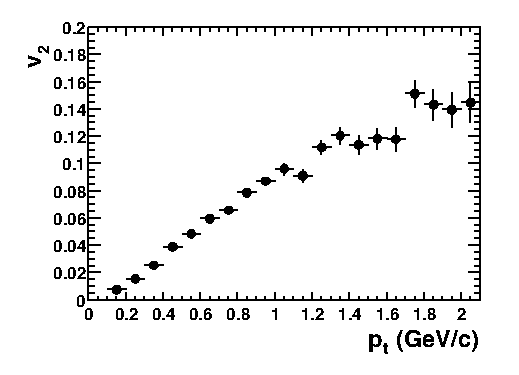
\includegraphics[width=0.45\textwidth]{Figures/Chapter1/STARV2Plot.eps}
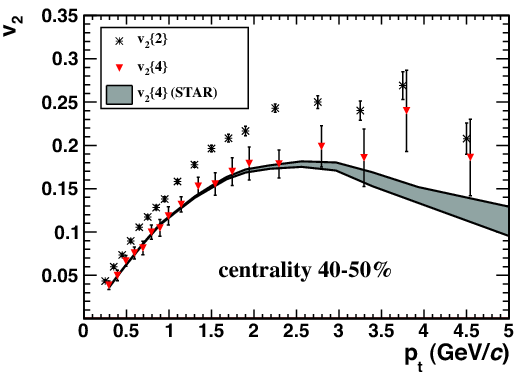
\includegraphics[width=0.45\textwidth]{Figures/Chapter1/ALICEV2Plot.png}
\caption{The elliptic flow of charged particles $v_2$ as a function of $p_T$ in AuAu collision measured by the STAR experiments at RHIC (left) and in PbPb collisions by the ALICE experiments at LHC (right) are shown above. Clearly, $v_2 > 0$ is observed in both experiments.}
\label{V2}
\end{center}
\end{figure}   

We can clearly see positive $v_2$ of charged particles at both RHIC and LHC, which also supports the creation of QGP in high energy heavy-ion collisions.  
 
\subsection{Strangeness Enhancement} 

As described in Section 1.4.6, the temperature of QGP is well above 100 MeV, which is much larger than the strange quark mass (about 95 MeV). Therefore, since $T_{QGP} > m_s$, in thermally and chemically equilibrated QGP, strange quarks could be produced thermally via the pair production process $u \bar u, d \bar d \rightarrow s\bar s$, and $gg \rightarrow s \bar s$, creating the chemical abundance equilibrium \cite{SSEnhance}. Therefore, the strangeness content in the QGP is enhanced, which could be experimentally observed from enhancement of strange particle yields in AA collisions compared to pp collisions. A direct experimental observable is the ratio of strange hadron yield to pions in AA and pp collisions. Figure \ref{PhiRAA1} and \ref{PhiRAA2} shows measurements on strange meson and baryons to pion ratios in AA and pp at RHIC and LHC 

\begin{figure}[hbtp]
\begin{center}
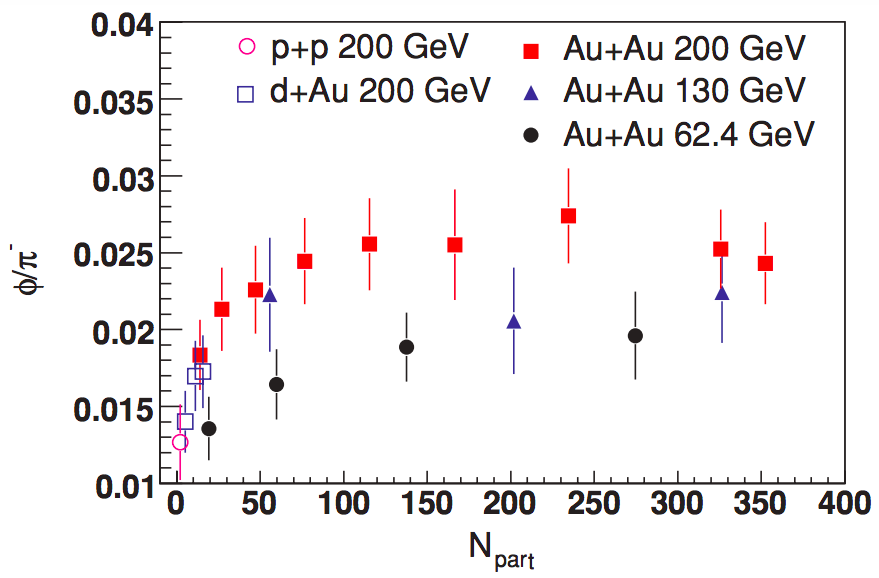
\includegraphics[width=0.45\textwidth]{Figures/Chapter1/STARPhiOverPi.png}
\caption{The yield ratio of $\phi/\pi$ as a function $N_{part}$ in p + p, p + Au, and Au + Au from the STAR experiment at RHIC are shown above.}
\label{PhiRAA1}
\end{center}
\end{figure}   

\begin{figure}[hbtp]
\begin{center}
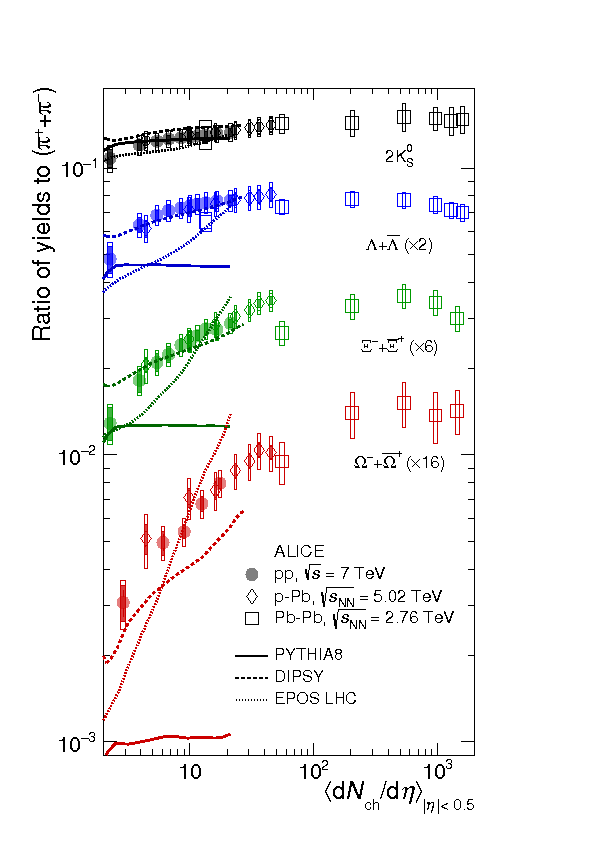
\includegraphics[width=0.60\textwidth]{Figures/Chapter1/ALICEStrange.png}
\caption{The yield ratio of strange hadrons $K^0_s, \Lambda^+, \Xi^0, \Omega^-$ as a function of $\langle dN_{ch}/d\eta \rangle$ from the ALICE experiment at LHC are shown above.}
\label{PhiRAA2}
\end{center}
\end{figure}   

We can see that $\phi/\pi$ ratio increases as $N_{part}$ and $\sqrt {s_{NN}}$ increases, which indicates strangeness enhancement in AA collisions compare to pp collisions. This again can be served as an evidence for the formation of QGP in heavy-ion collisions at RHIC and LHC. 

%J/psi suppression, jet quenching, elliptic flow, strangeness enhancement 

\subsection{Macroscopic Properties}

Physicists have conducted extensive studies to pin down macroscopic properties of QGP. 

\textbf{Transient Lifetime:} According to experimental results at RHIC and LHC, QGP has a very short lifetime. It is on the order of 10 fm/c \cite{QGPLifeTime}. It is generally assumed that QGP reaches thermal \cite{QGPThermal} and near chemical equilibrium \cite{QGPChemical} via the strong interaction. So far, there is not sufficient experimental evidence to directly support this assumption.

\textbf{Strong Interacting System:} Moreover, QGP, as a deconfined phase of matter, demonstrates a strongly interacting behavior, which contradicts to the prediction weak coupling according to the asymptotic freedom of quarks and gluons in QCD \cite{QCDAsym}. At $T \sim 1 - 3$ $T_c$, the coupling strength of QGP is still strong: $g_s \sim O(1)$ \cite{sQGP}. Therefore, strong interaction between the QGP constituents is in general non-perturbative. The equation of state of strong interacting QGP, as an input for hydrodynamic calculations, could be reasonably non-pertubative models such as MIT Bag Model or Lattice QCD \cite{LatticeEOS}. 

\textbf{Perfect Liquid Behavior:} Finally, QGP demonstrates a near-perfect liquid properties. The expansion of QGP in the fireball stage is approximately isentropic and could be well described by hydrodynamics \cite{Bjorken}. More specially, due to the relativistic nature of the strongly coupled near-perfect liquid system, assuming QGP reaches thermal \cite{QGPThermal} and near chemical equilibrium \cite{QGPChemical}, relativistic viscous hydrodynamics \cite{4DHydro} is the correct theoretical formalism for the dynamics of QGP. QGP is almost a perfect liquid. Its shear viscosity to entropy density ratio is very small: $\frac{\eta}{s}\sim (1 - 2.5) \frac{1}{4\pi}$ \cite{QGPEtaOverS}, approaching the quantum limit $\frac{\eta}{s} = \frac{1}{4\pi}$ predicted by the strongly coupled N=4 supersymmetric Yang-Mills plasma in Anti-de-Sitter Space/Conform Field Theory (AdS/CFT) correspondence \cite{ADSCFT}.

\textbf{Color Opaque Plasma:} It is also interesting that QGP is a color opaque plasma \cite{QGPGen}. This means that gluons propagating through the QGP will be absorbed by the plasma medium. Experimentally, the suppression of hadrons is a measure of the color opacity of the QGP \cite{QGPGen}. Physicists found that QGP is indeed highly color opaque \cite{QGPOpaque}.


%Nuclear Physics is a study of the interaction of nucleons and structure of atomic nuclei. 
%\subsection{Microscopic Structure}

%Constituents 

%Microscopic Kinetics -- Transport properties
 


\subsection{Open Questions}

Today, it has been more than 20 yeas since the discovery of QGP. However, there are still many outstanding conundrums, most of which are derived from the mysterious macroscopic behavior of QGP. Below is the list of selected open questions and are currently under active investigation by the heavy-ion physics community \cite{BigQuestions}:

1) \textbf{Thermalization of QGP:} How can QGP reach thermal equilibrium within such a short time, which is on the order 1 $fm/c$, from the non-equilibrium stage?

2) \textbf{Inner Workings of QGP:} What is the correct degree of freedom to describe QGP? The inner workings of QGP, as a deconfined phase of matter, must lay between asymptotically free quarks and gluons and color neutral hadrons. That is also why the sPHENIX experiment at RHIC, as the next generation DOE flagship Heavy Ion Physics program in the U.S., is going to built at BNL and collect date to probe the inner workings of QGP by resolving its properties at shorter and shorter length scales. 

3) \textbf{Smallest Droplet of QGP:} What is the smallest droplet of QGP that can be created? Can QGP be created in pPb, pp, or even $e^+e^-$ collision systems? What are the limits of the applicability of hydrodynamics?

\section{Heavy Flavor Physics}

\subsection{Heavy Quarks}

Heavy quarks, such as charm and beauty quarks, have large mass compared to the $\Lambda_{QCD}$ and $T_{QGP}$. Therefore, they are predominantly produced in early stage of heavy-ion collisions where hard scattering processes occur. Their production could be calculated by perturbation QCD. Figure \ref{HQProduce} show the lowest order Feynman diagrams of heavy quark pair production in QCD. 

 \begin{figure}[hbtp]
\begin{center}
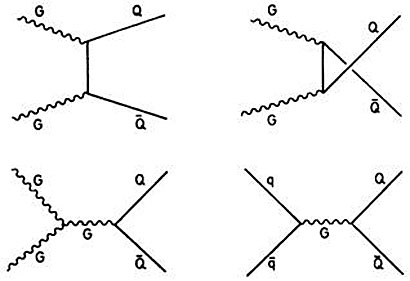
\includegraphics[width=0.45\textwidth]{Figures/Chapter1/HQDiagram.jpg}
\caption{The four lowest order tree level Feynman diagrams of heavy quark pair production are shown above.}
\label{HQProduce}
\end{center}
\end{figure}   

In general, due to their relatively momentum transfer to the medium constituents compared to mass \cite{}, they do not reach complete thermalization via multiple scattering as they traverse through the QGP. In addition, since their lifetime is much longer than the QGP lifetime, they retain their identities and record the evolution of the QGP, which makes them excellent probes. Then, they travel through the medium, hadronize into heavy flavor hadrons, and decay weakly. Their decay product are detected and identified by particles detectors.

Experimentally, from the final stage decay products, we can fully reconstruct open heavy flavor hadrons where heavy quark dynamics is encoded with different transverse momenta to study their diffusion coefficients, hadronizaton mechanism, and energy loss to probe the microscopic structure of QGP via their scattering patterns with the QGP constituents at different wavelengths. Figure \ref{HQ} below shows respectfully an event of beauty heavy quark production and hadronization in vacuum and QGP.

 \begin{figure}[hbtp]
\begin{center}
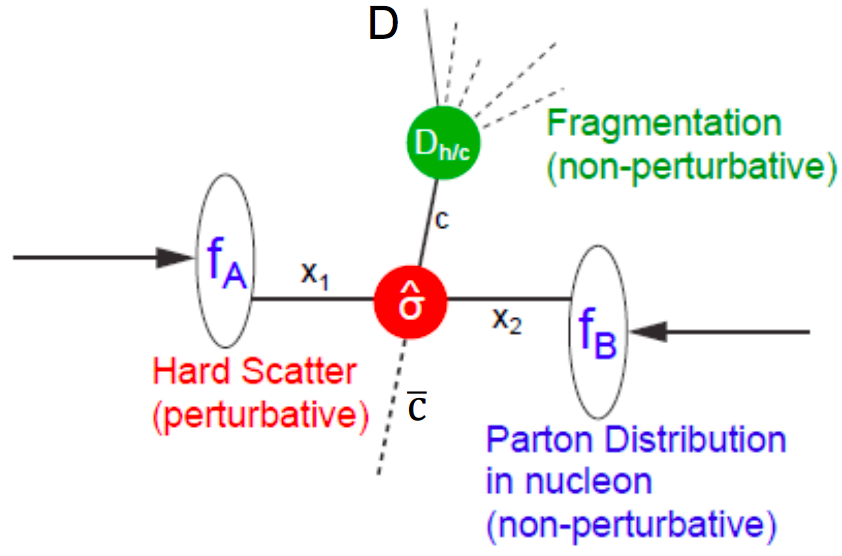
\includegraphics[width=0.46\textwidth]{Figures/Chapter1/HQVacuum.png}
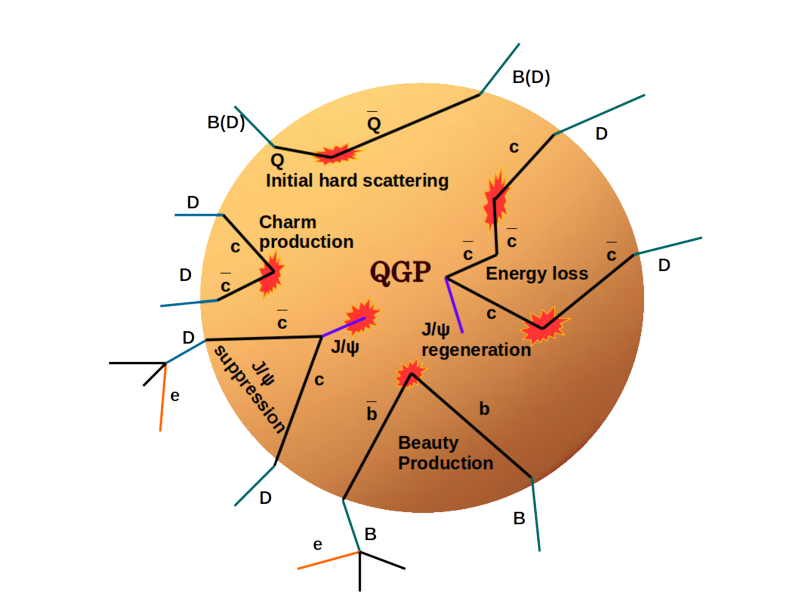
\includegraphics[width=0.48\textwidth]{Figures/Chapter1/HQQGP.png}
\caption{The schematic plots of heavy quark production and hadronization in vacuum (left) and QGP (right) are shown above.}
\label{HQ}
\end{center}
\end{figure}   


\subsection{Open Heavy Flavor Physics}

My graduate research focuses on answering the second question through the data analysis of fully reconstructed heavy flavor hadrons with the CMS experiment to understand transport properties and probe the microscopic structure of QGP. In this section, we will focus on discussing open heavy flavor physics where the only one heavy quark $Q$ is in hadron. Open heavy flavor hadrons have $\pm 1$ heavy flavor number. Quarkonia states $Q\bar Q$ are considered as hidden heavy flavor with a zero net heavy flavor quantum number. Their properties are different from open heavy flavor hadrons. We will not be discussed them in the follow subsections. 

\subsection{Heavy Flavor Physics in Vacuum}

To use heavy quark to probe the QGP created in heavy-ion collisions, we first need to understand heavy quark physics in vacuum from pp collisions. In the process $pp \rightarrow Q \bar Q$, QCD factorization theorem could be applied to study the using perturbative QCD (pQCD). Highn precision QCD calculations, including next-to-leading order (NLO), next-to-next-to-leading-order (NNLO), and Fixed-to-Next-to-the-Leading (FONLL), have been developed to describe heavy flavor production. Here, we will show FONLL calculation of the spectra of charm and beauty quarks, schematically denoted as: $\frac{d^2\sigma^Q}{p_T dp_T dy}$, in $pp \rightarrow Q  \bar Q$ at different energies \cite{FONLLRef}. Figure \ref{FONLL} shows the FONLL calculations of charm and beauty quarks spectra produced at the LHC energy for pp collisions at $\sqrt s = 5.02$ TeV.

 \begin{figure}[hbtp]
\begin{center}
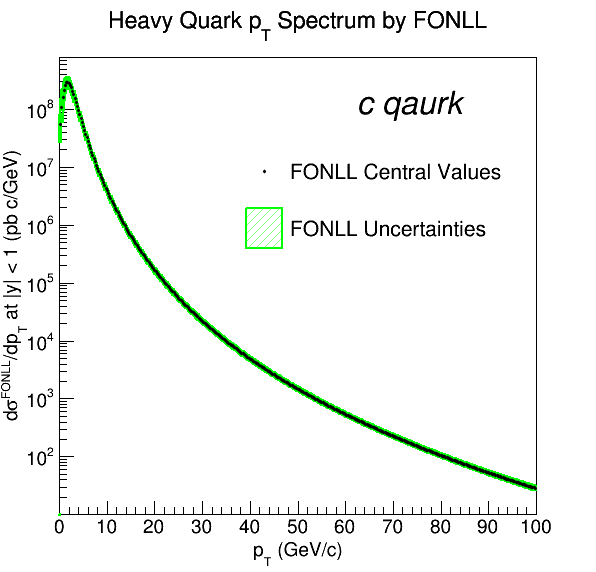
\includegraphics[width=0.45\textwidth]{Figures/Chapter1/Charm.png}
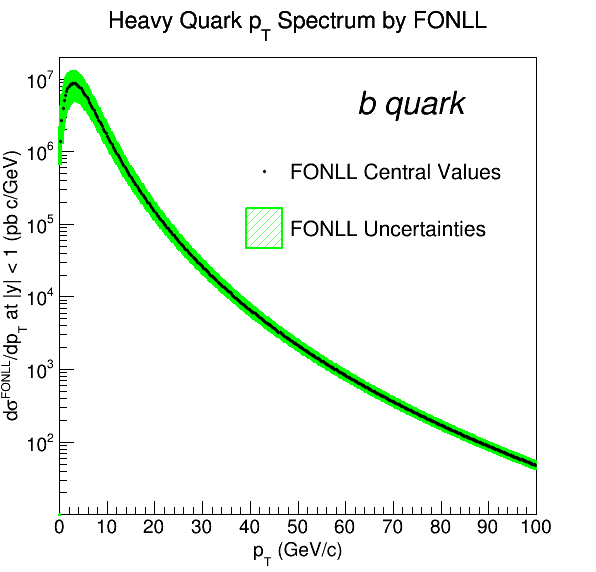
\includegraphics[width=0.45\textwidth]{Figures/Chapter1/Beauty.png}
\caption{The charm quark (left) and beauty quark (right) transverse momentum $p_T$ distribution at $\frac{d\sigma}{dp_T}$ at $|y| < 1$ from FONLL calculations are shown above.}
\label{FONLL}
\end{center}
\end{figure}   

In vacuum, heavy quarks fragment into heavy flavor hadrons $Q \rightarrow H_Q$. We can defined the parton fragmentation function $D^{H_Q}_{i}(z,\mu^2)$ where is the probability for a quark $q$ with energy $E$ fragment into a hadron with energy $zE$ ($0 < z < 1$) at the factorization scale of $\mu^2$ \cite{QCDFFunc}. According to pQCD, $D^{H_Q}_{i}(z,\mu^2)$ is universal in vacuum from $e^+e^-$, $ep$, and $pp$ collisions. Figure \ref{FFProcess} shows the scattering processes which fragmentation fraction is involved:

 \begin{figure}[hbtp]
\begin{center}
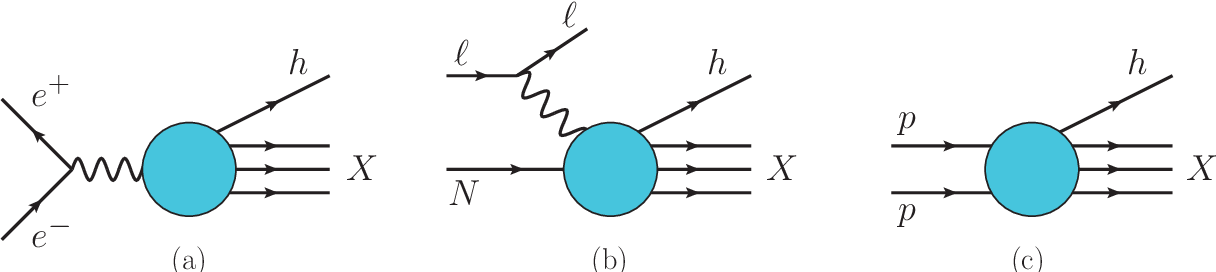
\includegraphics[width=1.0\textwidth]{Figures/Chapter1/FFProcess.png}
\caption{Single-inclusive hadron production process, where fragmentation function are involved, in (a) electron-positron annihilation, (b) deep-inelastic lepton-nucleon scattering, (c) proton-proton scattering are shown above.}
\label{FFProcess}
\end{center}
\end{figure}   

Next, we are ready to define heavy quark fragmentation fraction $f(Q \rightarrow H_Q)$. First we know, the energy

\begin{equation}
E=  \sqrt{m^2 + p_T^2 \cosh^2 y}
\end{equation}

Ignoring the mass, we have

\begin{equation}
E \simeq p_T \cosh y
\end{equation}

So energy of hadron $E^h$ that the quark with $E^Q$ fragmented to will be


\begin{equation}
E^h  = z E^Q 
\end{equation}

So we have the transverse momentum of the hadron $p_T^h$ 

\begin{equation}
p_T^{H_Q} = z p_T^Q
\end{equation}

With heavy quark spectra $ \frac{d^2\sigma^Q}{p_T dp_T dy}$ and parton fragmentation function $D_{i}^{H_Q}(z,\mu^2)$, we let


\begin{equation}
 \frac{d^2\sigma^Q}{p_T dp_T dy} = F^Q(p_T, y)
\end{equation}


Hence, for a hadron with $p_T$, the heavy quark will have $p_T/z$ with probability $D^{H_Q}_{i}(z)$ to fragment into this hadron. Therefore, the heavy flavor hadron spectra is given by:

\begin{equation}
\frac{d^2\sigma^{H_Q}}{p_T dp_T dy} = \int_{x_T}^1 F^Q(p_T/z, y) D_{i}^{H_Q}(z,\mu^2) dz
\end{equation}

Here $x_T = \frac{2p_T}{\sqrt s}$ \cite{HadronScale}.







\iffalse



From Figure \ref{FONLL} , it looks like the $p_T$ spectra of heavy quarks is overall approximately power law, particularly at high $p_T$. In fact, at a fixed $x_T$ and the center of mass angle \cite{HadronScale}, the heavy quark spectra overall demonstrates the power like behavior. In addition, assuming the spectra $F^Q(p_T,y)$ factorizes, we have
 

\begin{equation}
F^Q(p_T, y) \sim g(y) p_T^{-n}
\end{equation}

Hence,

\begin{equation}
F^Q(p_T/z, y) \sim F^Q(p_T, y)/z^{-n} = F^Q(p_T, y) z^n
\end{equation}


\begin{equation}
\frac{d^2\sigma^{H_Q}}{p_T dp_Tdy} \simeq \int_{x_T}^1 F^Q(p_T, y)  z^{n} D^{H_Q}_{i}(z) \frac{dz}{z^2} =F^Q(p_T, y)  \int_{x_T}^1  z^{n-2} D^{H_Q}_{i}(z) dz
\end{equation}



Hence, we can define the approximately constant heavy quark fragmentation fraction $f_{Q \rightarrow H_Q}$ as follows

\begin{equation}
f(Q \rightarrow H_Q) = \int_{x_T}^1 z^{n-2} D^{H_Q}_{i}(z) dz
\end{equation}

Hence, we will get 

\begin{equation}
\frac{d^2\sigma^{H_Q}}{p_T dp_T dy} = f(Q \rightarrow H_Q)  \frac{d^2\sigma^Q}{p_T dp_T dy}
\end{equation}

\fi

Now if we consider a factorization scaling near the heavy quark mass $\mu^2 \rightarrow m_Q^2$, according to PDG reference \cite{AlphaTheoEx}, solving the leading evolution equation, heavy quark fragmentation function $D_Q^{H_Q}(z)$ is in a form of delta function and light quark $q$ and gluons $g$ ($i = g, q$) will not contribute to produce heavy flavor hadrons. Hence, we could right

\begin{equation}
D^{H_Q}_{q,g}(z,\mu^2)|_{\mu^2=m_Q^2} = 0
\end{equation}

\begin{equation}
D^{H_Q}_{Q}(z,\mu^2)|_{\mu^2=m_Q^2} = f(Q \rightarrow H_Q) \delta(1 - z)
\end{equation}

Here $f({Q \rightarrow H_Q})$ is the heavy quark fragmentation fraction and stands for the probability of a heavy quark $Q$ hadronize into an open heavy flavor hadron $H_Q$. Indeed, according to the momentum sum rule constraint of the parton fragmentation function \cite{QCDFFunc}

\begin{equation}
\sum_{H_Q} \int_0^1 z D^{H_Q}_{Q}(z,\mu^2) dz = 1
\end{equation}

\begin{equation}
\sum_{H_Q} \int_0^1 z f(Q \rightarrow H_Q) \delta(1 - z) dz = 1
\end{equation}

\begin{equation}
\sum_{H_Q} f(Q \rightarrow H_Q) = 1 
\end{equation}

This verifies that the sum of heavy quark fragmentation fraction over all heavy flavor hadrons is equal to 1. Next, we have 


\begin{equation}
\frac{d^2\sigma^{H_Q}}{p_T dp_T dy} = \int_{x_T}^1 F^Q(p_T/z, y) D_{i}^{H_Q}(z,\mu^2) dz =  \int_{x_T}^1 F^Q(p_T/z, y) D^{H_Q}_{Q}(z,m_Q^2) dz 
\end{equation}

Thus,

\begin{equation}
\frac{d^2\sigma^{H_Q}}{p_T dp_T dy}  = \int_{x_T}^1 F^Q(p_T/z, y) f(Q \rightarrow H_Q) \delta(1 - z) dz =  f(Q \rightarrow H_Q)  F^Q(p_T, y)
\end{equation}

Hence, we have 

\begin{equation}
\frac{d^2\sigma^{H_Q}}{p_T dp_T dy} = f(Q \rightarrow H_Q) \frac{d^2\sigma^{Q}}{p_T dp_T dy}
\end{equation}

This means that the open heavy flavor hadron spectra $\frac{d^2\sigma^{H_Q}}{p_T dp_T dy}$ is essentially proportional to the heavy quark spectra $\frac{d^2\sigma^{Q}}{p_T dp_T dy}$ with heavy quark fragmentation fraction $f(Q \rightarrow H_Q)$ the as the coefficient of proportionality. Experimentally, charm and beauty fragmentation fractions have been measured at LEP, HERA, and the LHC and documented in PDG \cite{AlphaTheoEx}. The fragmentation fraction is often treated roughly a constant independent to $p_T$, $y$, and $\sqrt s$ and is assumed to be universal in $e^+e^-$, $ep$, and $pp$ collisions systems \cite{AlphaTheoEx}. 

In terms of being a constant, according LHCb $pp$ results \cite{LHCbFF}, it appears that the fragmentation fraction has significant $\sqrt s$ and $p_T$ dependence while no significant $y_B$ (or $\eta_B$) dependence is observed. Figure \ref{BeautyFFLHCb} shows the beauty quark fragmentation fraction: $f_u = f(b \rightarrow B^+)$, $f_d = f(b \rightarrow B^0)$, and $f_s = f(b \rightarrow B_s^0)$

 \begin{figure}[hbtp]
\begin{center}
\includegraphics[width=0.60\textwidth]{Figures/Chapter1/LHCbFFs.png}
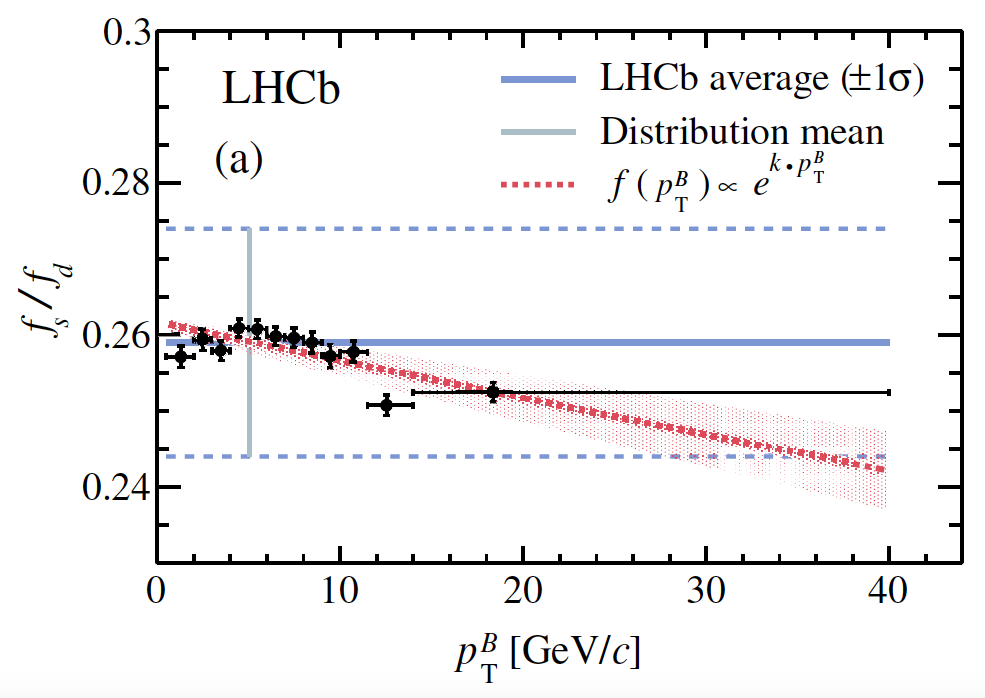
\includegraphics[width=0.60\textwidth]{Figures/Chapter1/LHCbFFpT.png}
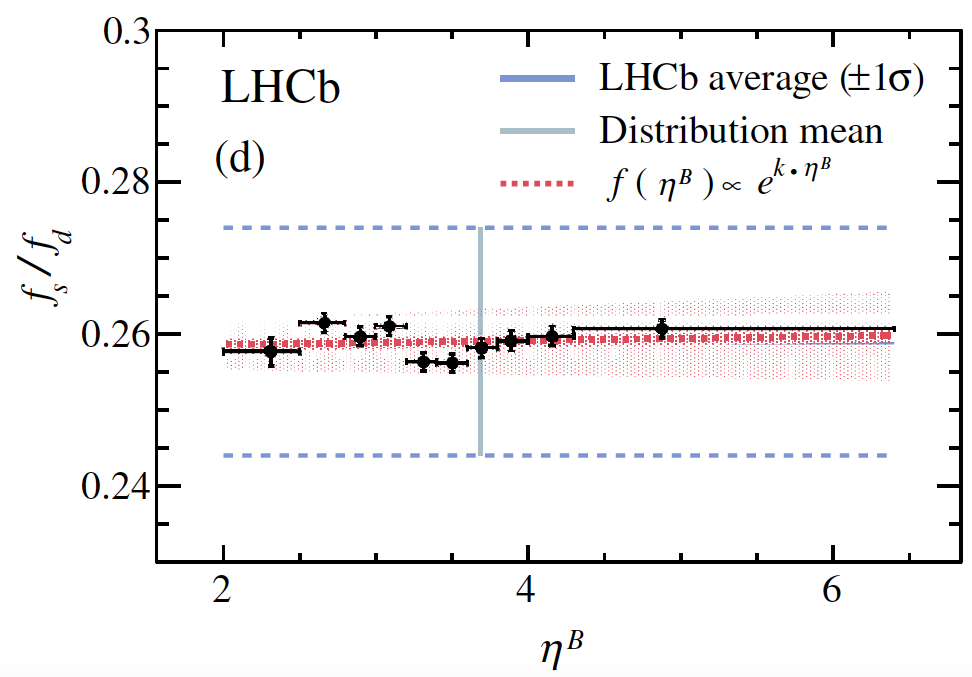
\includegraphics[width=0.60\textwidth]{Figures/Chapter1/LHCbFFy.png}
\caption{ $R$, the corrected yield ratio of $B^0_s/B^+$, as a function the $pp$ collision energy $\sqrt s$ (top), the $f_s/f_d$ ratio as a function $p_T$ (middle), and the $f_s/f_d$ ratio as a function $\eta_B$ (bottom), from the LHCb experiment are shown above.}
\label{BeautyFFLHCb}
\end{center}
\end{figure}   


In terms of universality, according to Strangeness Quark Matter Conference (SQM) in 2021, a hadronization universality breaking is observed from the ALICE experiment at the LHC \cite{GMISQM}. Figure \ref{CharmFFALICE} shows the hadronization universality breaking reported by the ALICE experiment in SQM 2021

 \begin{figure}[hbtp]
\begin{center}
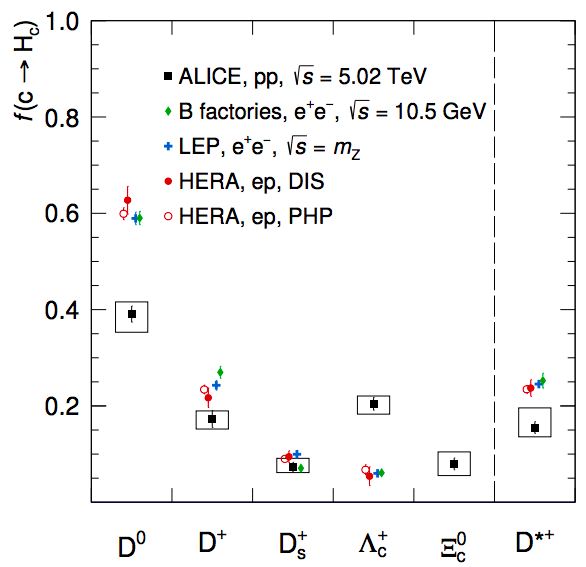
\includegraphics[width=0.52\textwidth]{Figures/Chapter1/ALICECharmFF.png}
\caption{The charm quark fragmentation fraction to different charm hadrons species in $e^+e^-$, $ep$, and $pp$ collisions are presented above. From the ALICE experiment, we can clearly see that the fragmentation fraction of $D^0$ has drop by about 40\% while the $\Lambda_c^+$ has enhanced by about a factor of 4. Therefore, the hadronization universality is clear broken at the LHC energy in the charm sector.}
\label{CharmFFALICE}
\end{center}
\end{figure}   

Further investigations of these results are currently ongoing. However, we will not expand the discussions here. Now, equipped with the understanding of heavy flavor physics in vacuum from $pp$ collisions as a reference, we are ready to use heavy quarks to probe the inner workings of QGP created in heavy-ion collisions. 

\subsection{Heavy Quark Diffusion}

In the limit of low $p_T$ or equivalently long wavelength, for heavy quarks inside the QGP medium, their elastic collision cross section dominates. In elastic $Q q \rightarrow Q q$ process in the thermally equilibrated QGP medium, heavy quarks has the relatively small momentum transfers of the order of the temperature compared to the heavy quark mass: $m_Q > |k| \simeq T$. Considering the mean free time of HQ in the QGP medium is about $\tau \sim 0.44 fm/c$ \cite{HQTau}. Therefore, the number of scattering of heavy quarks in the QGP medium is about $n \sim \frac{\tau_{QGP}}{\tau_{HQ}} \simeq 23 \sim O(10)$.

Now, we can consider a simple binomial process to model the diffusion of heavy quark in the QGP medium. Therefore, assuming the momentum of the heavy quark at $t = 0$ is $p$, after the time $\tau_{HQ}$, one scattering happens. The momentum of the heavy quark at $t = \tau_{HQ}$ either $p + k$ or $p - k$. Each has $1/2$ probability. Next, after another $\tau_{HQ}$, another scattering happens. The momentum of the heavy quark at $t = \tau_{HQ}$ either $p + 2k$, $p$ or $p - 2k$ with $1/4$, $1/2$, and $1/2$ probability respectfully. Therefore, the standard deviation of binomial process $\sigma_p = \frac{\sqrt{n}}{2} k$. If we take $n = 25$, $\sigma_p = 2.5k \simeq 2.5 T_{QGP} =$ 0.4 GeV. Experimentally, we consider a heavy quark with momentum about $p  > $ 1.5 GeV/c $>> \sigma_p$. 






We could see that the heavy quark transverse momentum is well above 1 GeV/c. Hence, such heavy quarks still retain a lot of memory about its initial conditions after multiple small scattering with QGP medium. Hence, in these conditions, heavy quark undergoes Brownian-like motion in the QGP medium \cite{HQReview}. Their motion in the QGP medium could be characterized by the Planck-Fokker Equation, which could be schematically written as follows \cite{HQRaff}:

\begin{equation}
\frac{\partial}{\partial t} f_q(t, \vec{p}) = \frac{\partial}{\partial p_{i}} \{ A_i(\vec p) f_q(t,\vec{p}) + \frac{\partial}{\partial p_j}[B_{ij}(\vec{p})f_q(t,\vec{p}) ] \}
\end{equation}

Here, $f_q(t,\vec{p})$ is the heavy quark phase space distribution function. If we ignore modification of the cold nuclear matter effect on the heavy quark initial production spectra, then in heavy-ion collision:

\begin{equation}
F^Q( t = 0,p_T) \propto \frac{d\sigma_{FONLL}}{p_Tdp_T}
\end{equation}


The transport parameters $A_i(\vec{p})$ is related to the thermal relaxation rate and $B_{ij}(\vec{p})$ is related to the momentum diffusion of heavy quark \cite{HQReview}. The heavy quark special diffusion coefficient $D_s$ is related to the transport parameter as follows:

\begin{equation}
D_s = \frac{T} {m_Q A(p=0)}
\end{equation}

$D_s$ characters the fundamental property of the QGP $\frac{\eta}{s}$ via the relationship 

\begin{equation}
2 \pi T D_s \simeq \frac{\eta}{s}
\end{equation}

More detailed studies has been carried out to examine heavy quark coupling strength and quantify the information heavy quarks carry as they traverse through the QGP medium \cite{HQJamie}.


\subsection{Heavy Quark Energy Loss}

In the limit of high $p_T$ or equivalently short wavelength, inelastic cross section starts to dominate \cite{}. Heavy quarks lose a substantial amount of energy as they travel fast through the QGP medium \cite{HQELossFirst}. In a simplified schematization, there are two different pictures that describe the energy loss mechanism of heavy quark in the QGP medium. In the pQCD picture, the coupling of the constituents of the QGP is assumed to be weak. Therefore, the QGP is made of weakly coupled quasiparticles. Heavy quarks scatter off the constituents incoherently when propagating through the QGP medium. There are two energy loss mechanisms: collisional energy loss and radiative energy loss \cite{HQRaff}. The collisional energy loss is given by $-\frac{dE}{dx} = \kappa_{coll}T^2$ and the radiative energy loss is given by  $-\frac{dE}{dx} = \kappa_{rad}T^3x$ \cite{HQCollELoss,HQRadELoss}. Figure \ref{HQELosspQCD} shows schematically heavy quark energy loss mechanism in the QGP medium



 \begin{figure}[hbtp]
\begin{center}
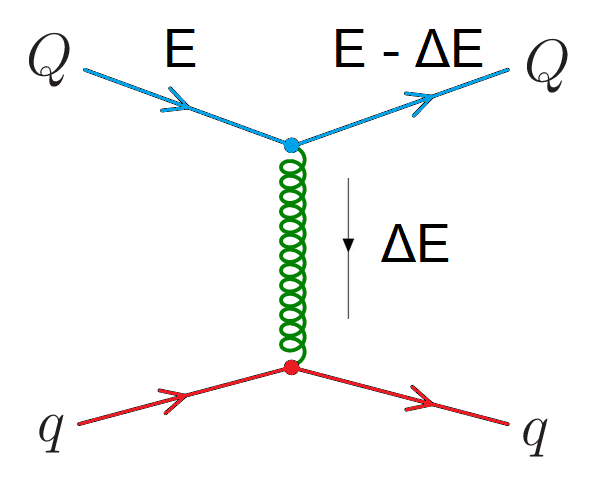
\includegraphics[width=0.35\textwidth]{Figures/Chapter1/Collisional.png}
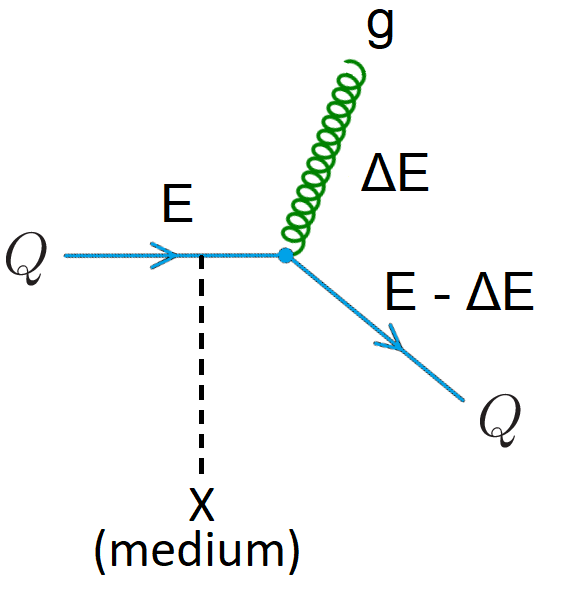
\includegraphics[width=0.35\textwidth]{Figures/Chapter1/Radiative.png}
\caption{The schematic demonstration of the pQCD picture: collisional energy loss (left) and radiative energy loss (right) of heavy quarks in the QGP medium are shown above.}
\label{HQELosspQCD}
\end{center}
\end{figure}   

The other picture, AdS/CFT, takes the strong coupling limit. In this picture, QGP behave like liquid and heavy quarks scatter off the constituents coherently in the QGP medium. The AdS/CFT model applies holographic drag force \cite{ADSCFTDrag} to calculate the energy loss of heavy quark \cite{HQHoloELoss} in the QGP medium

 \begin{figure}[hbtp]
\begin{center}
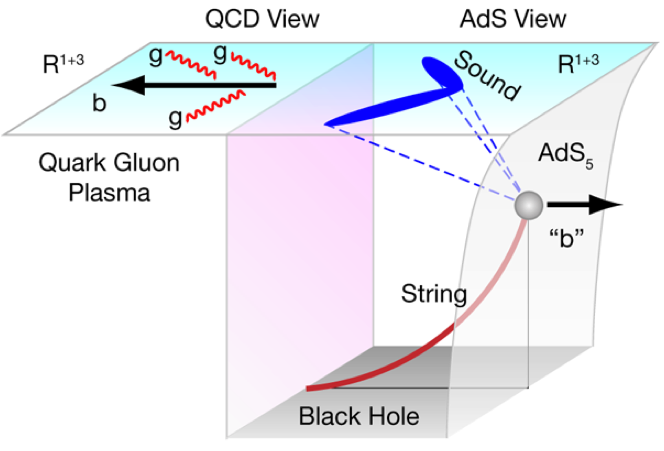
\includegraphics[width=0.45\textwidth]{Figures/Chapter1/ADSCFT.png}
\caption{The schematic demonstration of ADS/CFT picture: the energy loss of a quark in the QGP medium holographically due ADS/CFT drag force.}
\label{ADCCFT}
\end{center}
\end{figure}  

In pQCD picture, in the limit of $p_T \rightarrow \infty$, similar to electron Bremsstrahlung via QED radiation in the matter \cite{Brems}, for a heavy quark traveling through the QGP medium, its radiative energy loss via soft gluon radiation will dominate. The soft gluon radiation spectrum by a parton in the QGP medium is given by \cite{DEADCONE}

\begin{equation}
dP = \frac{\alpha_S C_{F}}{\pi} \frac{d\omega}{\omega}\frac{k_{\perp}^2 dk_{\perp}^2}{(k_{\perp}^2  + \omega^2\theta_0^2)^2}
\end{equation}

Where 

\begin{equation}
\theta_0 \equiv \frac{m}{E}
\end{equation}

Here, $\omega$ is the energy of the gluon and $k_{\perp}$ is the transverse momentum of the gluon, $C_F$ is color factor (Casimir) which is $3$ for gluons with one color and one anti-color charges and $4/3$ for quarks with one color charge. From Eq 1.84 above, a suppression of radiation at a small angle $0 - \theta_0$ is observed. This is effect is known as the dead cone phenomenon \cite{DEADCONE}. We also know that from from Eq 1.85, that as $m$ increases, the dead cone angle $\theta_0 = \frac{m}{E}$ will decrease. Figure \ref{DeadConePic} schematically shows a charm quark radiate gluon in the medium with a dead cone in the small angle:

 \begin{figure}[hbtp]
\begin{center}
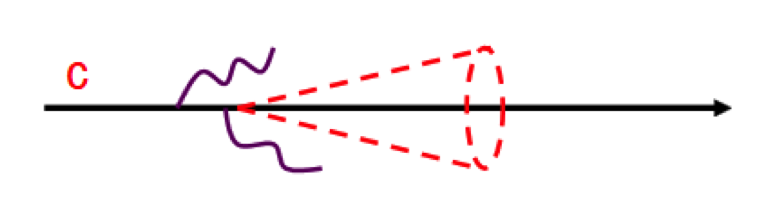
\includegraphics[width=0.85\textwidth]{Figures/Chapter1/CharmDeadCone.png}
\caption{The schematic demonstration of a charm quark radiate and suppression in small angle due to the dead cone effect in the QGP medium is shown above.}
\label{DeadConePic}
\end{center}
\end{figure}  

Since we have the follow mass hierarchy for quarks and gluons:

\begin{equation}
m_g < m_q < m_c < m_b
\end{equation}

We should expect the energy loss to follow

\begin{equation}
\Delta E_g > \Delta E_q > \Delta E_c >  \Delta E_b
\end{equation}

We call the inequality above to be the flavor dependence of energy loss, which is an important feature of heavy quark energy loss mechanism in the QGP medium. The studies of heavy quark energy loss mechanism in QGP will help us determine the fundamental jet transport coefficient $\hat q$ that characterizes the scattering power of the medium \cite{HQReview}. which relates to the mean free path and the momentum diffusion coefficient of heavy quarks \cite{qhatStudy}. The determination of $\hat q$ will be crucial for us decipher the inner workings of the QGP \cite{JetTransProbe}.

\subsection{Heavy Quark Hadronization}

After heavy quarks traverse through the medium, it will hadronize into heavy flavor hadrons, which could be fully reconstructed from their final state decay products in experiments. As described in section 1.2.7, in general, hadronization is non-perturbative. Considering heavy quark dynamics and apply hadronization models, physicists develop theoretical models to describe heavy quark hadrochemistry. Below, I will present two model candidates, the Texas A\&M University (TAMU) Model \cite{TAMUModel} and the Model developed from Cao et. al. \cite{CaoSunKo}, to describe beauty quark production and hadronization in vacuum:


\subsubsection{TAMU Model}

The TAMU Model uses a thermodynamic T-matrix formulism in terms of ``ladder diagrams'' to compute the heavy quark in-medium scattering amplitude and determine the non-perturbative transport parameters $A_i$ and $B_{ij}$ in the Planck-Fokker equation shown in Eq 1.81 \cite{TAMUModel}. Figure \ref{LadderDiagram} shows schematically the ``ladder diagram'' describing the dynamic evolution of a heavy quark in the QGP medium 

 \begin{figure}[hbtp]
\begin{center}
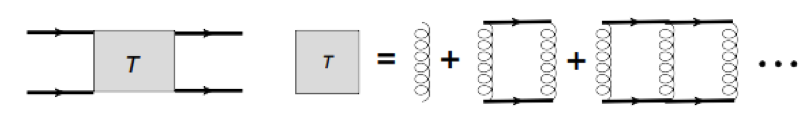
\includegraphics[width=1.0\textwidth]{Figures/Chapter1/LadderDiagram.png}
\caption{The ladder diagram used by the TAMU model to describe heavy quark diffusion in the QGP medium is shown schematically above.}
\label{LadderDiagram}
\end{center}
\end{figure}  

The input of T-matrix uses a lattice QCD potential \cite{LQCDTAMU} corrected with relativistic effects to model the non-perturbative interaction between heavy quarka and partons in the medium and make it consistent with HF spectroscopy in vacuum to determine the thermal relaxation rate coefficient $A_i(p,T)$. Only elastic collisional energy loss is included in the calculation. Resonance recombination model of heavy quark with a light quark nearby is applied to describe heavy quark hadronization \cite{RRM1}. Finally, effective hadronic scattering amplitudes is used to heavy flavor hadronic rescattering with other hadrons before kinetic freezout stage. The background parton composition and kinematics are modeled by the standard hydrodynamic simulations of the bulk medium in nuclear collisions

\subsubsection{Cao, Sun, Ko Model}

The Cao, Sun, Ko Model use an advanced Langevin-hydrodynamics approach \cite{CaoLH1,CaoLH2} incorporating both elastic and inelastic energy loss of heavy quarks inside the dynamical QGP medium. The equation below schematically shows relativistic Langevin equation to simulate heavy quark dynamics in the QGP medium


\begin{equation}
\Delta \vec{p} = - \gamma \frac{T^2}{M} \vec{p} \Delta t + \vec{\xi}(t) 
\end{equation}

And

\begin{equation}
\Delta \vec{x} = - \frac{\vec{p}}{E} \Delta t
\end{equation}

The noise is modeled by the Gaussian diffusion function 

\begin{equation}
P(\vec{\xi}) \propto \exp[\frac{\vec{\xi}^2}{2D_p \Delta t}]
\end{equation}

The dimensionless $\gamma$ factor is defined as

\begin{equation}
\gamma = \frac{M}{\tau_{HQ} T^2}
\end{equation}


A comprehensive coalescence model with strict energy-momentum conservation and PYTHIA fragmentation simulation \cite{PYTHIAFrag} with the default Peter fragmentation function, where the coalescence probability is determined from resonant scattering rate of heavy quarks in the QGP according to the resonant recombination model \cite{RRM1,RRM2}, are applied to model heavy quark hadronization.

In addition to TAMU Model and Cao, Sun, Ko Models, there are many other theoretical models that describe heavy quark hadrochemistry in heavy-ion collisions. Nevertheless, due to the large discrepancies between hadronization models, which significant limits the heavy-ion community to interpret the heavy flavor data. Therefore, experimentalists precisely measure heavy flavor observables and provide constrains for theoretical models.


 
\subsubsection{Equal Velocity Recombination Model}

In this model, the transverse momentum distribution of initially produced heavy quark is calculated by FONLL \cite{QCMModel}. The jet quenching effect in heavy-ion collisions is considered according to $R_{AA}$ measurement of $B^+$. The transverse momentum distributions of light-flavor quarks are obtained from data of light hadrons in the model. This model is particular designed to study low $p_T$ and mid-rapidity charm quarks produced at the LHC energy. It considers the equal-velocity combination of bottom quark with light-flavor anti-quarks  to form B mesons, a framework based on of co-moving quark recombination model (QCM).

\iffalse



\subsection{Experimental Observables}

Therefore, physicists propose many experimental observables to study open heavy flavor physics and test theoretical models in heavy ion collisions. Traditionally, heavy flavor hadron $v_2$, $R_{AA}$, and yield ratio are extensively studied. 

\textbf{Heavy Quark Diffusion: $v_2$}

In the QGP medium, heavy quark diffused by the color force and multiple scatter with medium constituents, which could generate sizable azimuthal anisotropy $v_2$ \cite{HQReview}. Experimentally, we scale the $v_2$ and the hadron kinetic energy $K_T = \sqrt{m^2 + p_T^2} - m^2$ of heavy quarks with $n_q$ according to the Number of Constituent Quark (NCQ) Scaling in quark coalescence model \cite{NCDScaling}. Figure \ref{HQV2} shows the comparison of the $v_2/n_q$ as a function of $K_T/n_q$ of $D^0$ ($c\bar u$) meson with light flavor hadrons with STAR experiments at RHIC \cite{STARD0v2} and the CMS experiment at LHC \cite{CMSD0v2}.


\begin{figure}[hbtp]
\begin{center}
\includegraphics[width=0.50\textwidth]{Figures/Chapter1/STARv2.png}
\includegraphics[width=0.485\textwidth]{Figures/Chapter1/CMSv2.png}
\caption{The NCQ scaled $D^0$ $v2/n_q$ vs $K_T/n_q$ and the comparison light hardons measured by the STAR experiment at RHIC (left) and the CMS experiment at LHC (right) are shown above.}
\label{HQV2}
\end{center}
\end{figure}   

We could see a reasonably good NCQ scaling behavior of $D^0$ meson with other light flavor hadrons, which suggests sizable collectivity of charm quarks in the QGP medium.

\textbf{Heavy Quark Energy Loss Mechanism: $R_{AA}$}

As we mentioned previously, the nuclear modification factor $R_{AA}$ of heavy flavor hadrons as a function of $p_T$ could quantify the energy loss of quarks via the shift of the $p_T$ spectra to the left in $AA$ collisions compared to $pp$ collisions. Figure \ref{HQRAA} $R_{AA}$ heavy and flavor hadrons measured with experiments at RHIC and LHC.

\begin{figure}[hbtp]
\begin{center}
\includegraphics[width=0.47\textwidth]{Figures/Chapter1/STARRAA.eps}
\includegraphics[width=0.47\textwidth]{Figures/Chapter1/CMSRAA.png}
\caption{The $D^0$ $R_{AA}$ vs $p_T$ with the STAR experiment in 0 - 10\%, 10 - 40\%, and 40 - 80\% centrality at RHIC and the $D^0$, $B^+$, non-prompt $J/\psi$ and charged hadrons $R_{AA}$ vs $p_T$ at at 0 - 100\% centrality with the CMS experiment at LHC are shown above.}
\label{HQRAA}
\end{center}
\end{figure}   

We could see that $R_{AA}$ of $D^0$ and $B^+$ are both below 1, which suggest charm and beauty quarks lose a significant fraction of energy to the QGP medium. As $p_T$ increases, the $R_{AA}$ of light and heavy flavor hadrons converge to the same value and approach 1, which Lorentz $\gamma$ factor come into play where the mass of the hadron become irrelevant. In addition, the CMS results above indirectly agree with the expectation of the flavor dependence of energy loss: $R_{AA}^{h} < R_{AA}^{D} < R_{AA}^{B} < 1$. With both $R_{AA}$ and $v_2$, we can constrain theoretical models and understand the interaction mechanism of heavy quarks with the QGP medium.

\textbf{Heavy Quark Hadronization: $H_s/H^0$ and $\Lambda_{Q}/H^{0}$}

According to the theoretical reviews of heavy quarks hadrochemistry in heavy-ion collisions \cite{StrangetoLight,BaryontoMeson}, the strange-to-non-strange meson ($H_s/H^0$) and baryon-to-meson ($\Lambda_{Q}/H^{0}$) ratios are excellent observables to test hadronization models. Figure \ref{HadroPlotCharm} shows the fully reconstructed $\Lambda_C^+/D^0$ ratio measured by the STAR and CMS experiments

\begin{figure}[hbtp]
\begin{center}
\includegraphics[width=0.52\textwidth]{Figures/Chapter1/STARLambdaCD0.png}
\includegraphics[width=0.47\textwidth]{Figures/Chapter1/ALICELambdaCD0}
\caption{The fully reconstructed $\Lambda_C^+/D^0$ ratio in pp and heavy-ion collisions measured by the STAR experiment at RHIC (left) and the CMS experiment at LHC (right) are shown above.}
\label{HadroPlotCharm}
\end{center}
\end{figure}   

We can see that in general, $\Lambda_C^+/D^0$ ratio in heavy-ion collisions lies above its ratio in $pp$ collisions. Moreover, there are many different theoretical predictions agree reasonably well with the experiments due to the large uncertainties. More precise $\Lambda_C^+/D^0$ measurements will be desired in order to constrain theoretical models.

In addition to $v_2$, $R_{AA}$, and $\Lambda_{Q}/H^{0}$, some modern observables with more differentiation such as the hadron-hadron correlation and heavy flavor jet substructure measurements have been recently carried out \cite{DDbar,DJet}. 

Hence, with the motivation to understand the hadronization mechanism of heavy quarks and investigate the inner workings of the QGP, I propose to carry out open heavy flavor physics measurements. In this thesis, I will focus on the measurement of the experimental observable $B^0_s/B^+$ ratio from fully reconstructed $B^0_s$ and $B^+$ mesons (and their anti-particles) via decay channels of $B^0_s \rightarrow J/\psi \phi \rightarrow \mu^+ \mu^- K^+ K^-$ and $B^0_s \rightarrow J/\psi K^+ \rightarrow \mu^+ \mu^- K^+$ in pp and PbPb collisions with the CMS experiment at the LHC to study the beauty production and hadronization mechanism in vacuum and QGP. 



\fi

%% %% This is an example first chapter.  You should put chapter/appendix that you
%% write into a separate file, and add a line \include{yourfilename} to
%% main.tex, where `yourfilename.tex' is the name of the chapter/appendix file.
%% You can process specific files by typing their names in at the 
%% \files=
%% prompt when you run the file main.tex through LaTeX.
\chapter{The CMS Detector}

\section{Overview}

The Compact Muon Solenoid (CMS) Detector is a general purpose high-energy physics detector located 100 meters underground on the French side of the LHC \cite{CMSDetector}. Overall, the complete detector is 21 m long, 15 m wide and 15 m high with a weight of 14 kiloton, heavier than the Eiffel Tower in Paris. It functions as a giant, high-speed camera, taking 3D ``photograph'' of particle collisions from all directions up to 40 million times each second. Figure \ref{CMSRealPic} shows the photo taken for the CMS detector at the underground collision hall.

\begin{figure}[hbtp]
\begin{center}
\includegraphics[width=0.80\textwidth]{Figures/Chapter2/CMSRealPic.jpg}
\caption{The front view of the CMS detector at the underground collision hall is shown above.}
\label{CMSRealPic}
\end{center}
\end{figure} 

The CMS detector is made of sub-detectors including silicon strip and pixel trackers, the preshower made of silicon strips, the crystal electromagnetic calorimeter (ECAL), the superconducting solenoid with 3.8 T of magnetic field strength, the inner hadronic calorimeter (HCAL), the steel returning yoke to enhance the magnetic field strength, the outer hadronic calorimeter, the muon chambers, and the forward hadronic calorimeter \cite{CMSDetector}. Figure \ref{CMSDecPic} shows schematic view of the CMS detector

\begin{figure}[hbtp]
\begin{center}
\includegraphics[width=0.80\textwidth]{Figures/Chapter2/CMSDecPic.jpg}
\caption{The schematic view of the CMS detector with brief descriptions of all its components is shown above. Image from \cite{HiggsCMS}}
\label{CMSDecPic}
\end{center}
\end{figure} 

The CMS detector is built, operated, and maintained by the CMS Collaboration. The CMS Collaboration consists of over 4000 members including scientists, engineers, technicians, students, and administrative assistants from 200 institutes and universities in 40 countries around the world. Physicists take data from the CMS detector and share data with each other with online system. The data are store in tapes and kept at different institutions. Members of the CMS experiment collaborate with each other on detector studies and data analysis to produce important scientific results and have published in more than 1000 papers in internationally recognized journals.

In the following sections, I will describe in more details the CMS experiment including the trigger system for data acquisition, the tracking system to track charged particles, the muon system for muon detection, identification, and reconstruction, and the calorimeter system to measure the energy of the particles.

\section{Triggers}

The CMS experiment develops triggers to acquire experimental data \cite{CMSTrigger}. Its main purpose is to select events of potential physics interests from approximately one billion events per second the particles collisions at the LHC. The CMS trigger system consists of two levels of triggers: hardware level 1 (L1) trigger and the software high level trigger (HLT). Different triggers encoded in the L1 and HLT are designed and fire to collect datasets for specific physics studies.

\subsection{L1 Trigger}

In the CMS experiment, an event is defined as a snapshot of one collision at the LHC. In the L1 trigger, physicists develop algorithms according to detector electronics response to decide if an event is accepted or rejected within the L1 trigger latency time. Figure \ref{L1Overview} shows the schematic overview of L1 trigger making its decision online to select events based on the information from the calorimeter and muon systems.


\begin{figure}[hbtp]
\begin{center}
\includegraphics[width=0.50\textwidth]{Figures/Chapter2/L1Overview.png}
\caption{The figure above demonstrates how the CMS L1 hardware trigger function schematically.}
\label{L1Overview}
\end{center}
\end{figure} 

In the interest of heavy-ion studies, physicists develop a set of dedicated triggers algorithms in the L1 trigger to build datasets. The minimum biased (MB) trigger is designed to collect minimum bias data for elliptic flow, $D^0$ meson, and charged particle multiplicity analyses while the single muon trigger is designed to select events muons for heavy flavor and electroweak physics analyses. We will describe the MB trigger since we will need to use it to determine the number of MB events in our analysis.

\subsection{MB Trigger}

By definition, an MB event corresponds to a non-single diffractive inelastic interaction \cite{MBTrigger}. A totally inclusive trigger, or called zero bias (ZB) trigger, corresponds to a randomly reading out from the detector whenever a collision is possible. MB trigger is algorithm to determine interesting MB events based on the response from forward HCAL located at $3 < |\eta| < 5$. It is put a fixed analog to digital converter (ADC) threshold in the HCAL response to reject background noise and collect MB events from ZB trigger. There is also an essentially linear relation between the maximum ADC with the actual energy response of the forward HCAL. Figure \ref{HFADC} shows the ADC distribution and HF energy as a function of ADC in 2018 PbPb run.

\begin{figure}[hbtp]
\begin{center}
\includegraphics[width=0.45\textwidth]{Figures/Chapter2/AllADC.png}
\includegraphics[width=0.45\textwidth]{Figures/Chapter2/HFvsADC.png}
\caption{In the CMS 2018 PbPb Run 326791, the ZB data (red), Empty Bunches (blue), and MB data (green) ADC distributions (left), and the HF energy according to the charge collected as a function of ADC (right) are shown above. We can see that the HF energy  is about (0.5 - 1) conversion factor to the ADC.}
\label{HFADC}
\end{center}
\end{figure} 

The MB trigger consist ``MB OR'', which requires the ADC threshold on either one of the forward HCAL (HF) out of both forward ECAL in both positive and negative sides, and ``MB AND'',  which requires the ADC threshold on both of HFs out of both forward ECAL in both positive and negative sides. Figure \ref{2018PbPbMB} shows the L1 MB trigger analysis of Run 326791 in the 2018 CMS PbPb data taking 

\begin{figure}[hbtp]
\begin{center}
\includegraphics[width=0.45\textwidth]{Figures/Chapter2/MaxADC.png}
\includegraphics[width=0.45\textwidth]{Figures/Chapter2/MBTrgEffADC.png}
\caption{In the CMS 2018 PbPb Run 326791, the ZB data (red), Empty Bunches (blue), and MB data (green) maximum ADC distributions (left) and the efficiencies of MB OR (blue) and MB AND (red) as a function ADC threshold (right) are shown above.}
\label{2018PbPbMB}
\end{center}
\end{figure} 

In the 2018 CMS PbPb data taking, to reject the noisy background, the max ADC of each event is required to be greater than 15 with MB AND along with the HLT trigger of at least one pixel track are applied to select MB events, as seen above from Figure \ref{2018PbPbMB} in the max ADC distribution of MB evens in green. A total number of about 2.4 billion MB events corresponding to a luminosity about 1.7 $nb^{-1}$ have been collected by CMS during the 2018 LHC PbPb run from November to December 2018. Figure \ref{MBStat} shows the MB events and corresponding luminosity as a function day throughout the 2018 CMS PbPb data taking period

\begin{figure}[hbtp]
\begin{center}
\includegraphics[width=0.55\textwidth]{Figures/Chapter2/MBStat.pdf}
\caption{The figure above shows the total number of 20 PbPb MB events from and corresponding luminosity how the as a function Run ID from November 15 to December 2 2018.}
\label{MBStat}
\end{center}
\end{figure} 


\subsection{Centrality Efficiency with MB Trigger}

In addition to overall efficiency vs the ADC with the MB trigger, we also study the centrality efficiency with different ADC thresholds. Figure \ref{EffCent} shows the centrality as a function of efficiency using MB OR and MB AND with different thresholds

\begin{figure}[hbtp]
\begin{center}
\includegraphics[width=0.55\textwidth]{Figures/Chapter2/EffCent.png}
\caption{The efficiency vs centrality with ADC > 16 for MB OR (blue) and MB AND (green) are shown above.}
\label{EffCent}
\end{center}
\end{figure} 

Because other physics trigger are mainly based on the MB datasets, in the physics analyses using 2018 CMS PbPb datasets, it is recommended to remove the very peripheral centrality range from 90 - 100\%, which is not fully efficient (efficiency $<$ 100\%). Therefore, the most of the CMS heavy-ion physics results using the 2018 PbPb dataset will be presented in the centrality range of 0 - 90\%.

\subsection{HLT Trigger}

The HLT software trigger is an array of commercially available computers running high-level physics algorithms \cite{CMSTrigger}. Unlike the online L1 hardware trigger which runs on-the-go during the data taking process, HLT is an offline software trigger that runs after the data are acquired. In the HLT trigger, more sophisticated analyses are performed to determine if the event is accepted or rejected for a specific dataset. The event data are stored locally on disk and eventually transferred to downstream systems, the CMS Tier-0 computing center, for offline HLT processing and permanent storage \cite{CMSTrigger}. There are many trigger paths in the HLT such as the high multiplicity trigger to specifically collect events with many tracks, the D meson trigger to select high $p_T$ D mesons, and the dimoun trigger to enrich Drell-Yen events, are designed and encoded in the HLT trigger. In the following, we will describe the dimuon trigger in details because the dimuon dataset will be used to fully reconstruct B mesons in this thesis. 

\subsection{DiMuon Trigger}

The dimuon trigger, as it is named, is a trigger based on the information of two muons tracks. HLT is able to quickly reconstruct the invariant mass of two oppositely charged muons $m_{\mu\mu}$. Figure \ref{DimuonInvMass} shows the $m_{\mu\mu}$ reconstructed by the CMS HLT with 2018 pp dataset.

\begin{figure}[hbtp]
\begin{center}
\includegraphics[width=0.55\textwidth]{Figures/Chapter2/DimuonInvMass.png}
\caption{The dimuon invariant spectrum $m_{\mu\mu}$ reconstructed by CMS HLT trigger in the 2018 pp dataset is shown above. We can identify the neutral vector boson resonances shown above.}
\label{DimuonInvMass}
\end{center}
\end{figure} 


In the 2018 PbPb run, the dimuon trigger requires the presence of two muon candidates, with no explicit momentum threshold and with the HLT reconstructed dimuon invariant mass of 1.0 GeV/c$^2$ $< m_{\mu\mu} <$ 5.0 GeV/c$^2$, near the $J/\psi$ PDG mass $m_{J/\psi} =$ 3.0969 GeV/c$^2$ \cite{AlphaTheoEx}, in coincidence with lead bunches crossing at the interaction point. Moreover, One of the trigger-level muons is reconstructed using information both from the muon detectors and the inner tracker with requirement of more than or equal to 10 hits (named as L3 muon), while for the other only information from the muon detectors is required (named as L2 muon) \cite{BAnaDimuonTrigger}.

\section{Tracking System}

\subsection{Silicon Detectors}

The CMS tracking system applies solid state semiconductor technologies. It consists of the 3 layers of silicon pixel tracker and 10 layers of silicon strip detector including 4 inner barrel layers and 6 outer barrel layers \cite{CMSSilicon}. It have a $\phi = 2\pi$ and $|\eta| < 2.4$ acceptance coverage. Figure \ref{CMSTracker} shows the CMS tracking system schematically

\begin{figure}[hbtp]
\begin{center}
\includegraphics[width=0.80\textwidth]{Figures/Chapter2/CMSTrackingSchemtic.png}
\caption{The schematic view of the CMS tracking system is shown above.}
\label{CMSTracker}
\end{center}
\end{figure} 


In nuclear and particle physics, a tracker is a detector that measures the trajectories of charged particles via ionization. In general, it does not destroy or significantly change the energy of the particle. With the external magnetic field, the tracker can measure the momentum, the charge, and the mass of the particle by the studying the electric charges collected from electron avalanche or electron-hole pair. The CMS tracking systems provides physicists with excellent tracking capabilities. The CMS silicon tracker is solid state detector employing semiconductor technologies. The silicon tracker is operated at a reserve bias mode with a depletion voltage of about 600V. High energy charged particles passing through the silicon tracker has an energy loss of $dE/dx \simeq 0.5 keV/\mu m$ \cite{AlphaTheoEx}. Therefore, for a 320 $\mu m$ thick silicon sensor, the charged particle will lose about 160 keV. The electron-hole pair in silicon is about 3 eV per pair. Therefore, the charged particle will produce roughly on the order of $10^4$ electrons. The hit resolution in $r\phi$ direction of the silicon strip is about 10 -- 40 $\mu m$ \cite{CMSTrackComp}. Figure \ref{SiliconDetector} shows schematically how a high energy charged particle ionized a electron-hole pair in the depletion region of a silicon P-N junction diode operated at a reverse biased mode


\begin{figure}[hbtp]
\begin{center}
\includegraphics[width=0.75\textwidth]{Figures/Chapter2/SiliconDetector.png}
\caption{The schematic plot explaining how a silicon tracker detector charged particles is shown above.}
\label{SiliconDetector}
\end{center}
\end{figure} 

However, in the CMS silicon tracker, due to the small number of electrons produced in the silicon sensor, the energy loss $dE/dx$ vs momentum $p$ of charged particle is does not good enough resolution to separate and identify electron, pion, kaons and protons. Therefore, we generally do not perform particle identification (PID) for hadrons with CMS detector in physics analyses.  

\iffalse

\subsection{Tracking Algorithm}

With the hardware silicon tracker, the CMS collaboration also developed the state-of-the-art tracking algorithm to reconstruct the paths and primary vertices of the collisions from the electronic readout signals. CMS tracking algorithm employs the Combinatorial Track Finder (CTF), an adaptation of the combinatorial Kalman filter \cite{CMSTrack1,CMSTrack2,CMSTrack3}, which in turn is an extension of the Kalman filter \cite{Kalman} to allow pattern recognition and track fitting to occur in the same framework. The collection of reconstructed tracks is produced by multiple passes (iterations) of the CTF track reconstruction sequence, in a process called iterative tracking \cite{CMSTrackComp}. The CMS tracking workflow and its performance are shown in Figure \ref{TrackWorkFlow} and Figure \ref{CMSTrackPer}

\begin{figure}[hbtp]
\begin{center}
\includegraphics[width=0.90\textwidth]{Figures/Chapter2/TrackWF.pdf}
\caption{The schematic block diagram of CMS tracking workflow is shown above.}
\label{TrackWorkFlow}
\end{center}
\end{figure} 


%Figure \ref{CMSTrackPer} shows the general performance of CMS tracking algorithm

\begin{figure}[hbtp]
\begin{center}
\includegraphics[width=0.48\textwidth]{Figures/Chapter2/TrackPTEff.pdf}
\includegraphics[width=0.48\textwidth]{Figures/Chapter2/TrackPTFake.pdf}
\caption{The CMS tracking efficiency (left) and fake rate (right) as a function of $p_T$ from simulations of $t \bar t$ events at 13 TeV with different pileup conditions are shown above.}
\label{CMSTrackPer}
\end{center}
\end{figure} 

Finally, with the collection of tracks, assuming all the tracks are promptly produced at a given interaction point, we can determine the primary vertex by selecting the tracks, performing track clustering, and fitting for the position of each vertex using its associated tracks \cite{CMSTrackComp}. The deterministic annealing algorithm \cite{DAAlgo} is track clustering algorithm that CMS is currently using. The track and vertex information of each event will be stored in datasets for physics analyses.

\fi

\section{Muon System}

Named as ``Compact \textbf{Muon} Solenoid'', the study on muon is one of the most important physics tasks of the CMS experiment. The CMS muon system has 1400 muon chambers including 250 drift tubes and 540 cathode strip chambers to track the positions of the muons and provide a trigger and 610 resistive plate chambers form a redundant trigger system with an acceptance coverage of $|\eta| < 2.4$ . Due to the small energy loss of muon in ECAL and HCAL \cite{AlphaTheoEx}, the muon produced from the collisions usually penetrates through the trackers and calorimeters. Therefore, the muon system is located at the outer of the CMS detector. Figure \ref{ParticleFlow} shows the particles produced at the interaction points and pass through the CMS detector

\begin{figure}[hbtp]
\begin{center}
\includegraphics[width=0.90\textwidth]{Figures/Chapter2/CMSParticleFlow.png}
\caption{The particle flow of long life particles, such as electrons, muons, photons, charged hadrons: $\pi,K,p$, and neutral hadrons: neutrons, in the CMS detector are shown above.}
\label{ParticleFlow}
\end{center}
\end{figure} 

%\textbf{How MUON CHAMBER WORKS}

The muon system employs gaseous detector technology. Physical modules of drift tubes, cathode strip proportional planes, and resistive plates are called ``chambers''. When a muon pass through the chambers, it will ionize electrons of the gas atom. Under a strong electric field, the avalanche electrons will be drifted to the anode and the gas ion will be drifted to the cathode. Electronic signal will be generated as this occurs. Figure \ref{Muonsystem} shows schematically how electron avalanches works in a gaseous detector to detect charged particles as well as the design of CMS drift tube to detect muons.


\begin{figure}[hbtp]
\begin{center}
\includegraphics[width=0.85\textwidth]{Figures/Chapter2/EAva.png}
\includegraphics[width=0.85\textwidth]{Figures/Chapter2/CMSDT.png}
\caption{A visualization of Townsend Avalanche (top) and schematic plot of the CMS drift tube detecting a muon (bottom) are shown above.}
\label{Muonsystem}
\end{center}
\end{figure} 


%The muon in the tracker uses a similar tracking algorithms as other charged particles \cite{CMSTrackComp}. Muon tracking performance is excellent. For isolated muons with 1 < $p_T$ < 100 GeV/c, the tracking efficiency is $>$ 99\% over the full $\eta$-range of tracker acceptance and does not significantly depend on $p_T$ while the fake rate is negligible \cite{CMSTrackComp}. We can require hits on the outer most muon chambers to identify muons because other charge particles will be stopped by the calorimeter and should not be able to enter the muon system as shown on Figure \ref{ParticleFlow}. Therefore, the CMS muon system has excellent capabilities of detecting, identifying, and reconstructing muons, which is crucial for heavy flavor physics studies. 

Therefore, with both the tracking system and the muon chambers, the CMS detectors has excellent capabilities of detecting, identifying, and reconstructing muons, which is crucial for heavy flavor physics studies.

\section{Calorimeter System}

In nuclear and particle physics, a calorimeter is a detector that completely stops particles and measure the total energy deposited. According to the particles, calorimeter can be divided into electromagnetic calorimeter (ECAL or EMCAL) to measure the energy of electron and photons and hadronic calorimeter to measure the energy of charge and neutron hadrons. The CMS calorimeters system includes both ECAL and HCAL. It is located in between the tracker and the muon chambers as shown in Figure \ref{CMSDecPic}. 

According to measurement of charged particle shower energy, calorimeter can typically be classified as sampling calorimeter and homogenous calorimeter. The sampling calorimeter has two components: absorber and scintillator. Absorber is generally made of metals and produces the shower. The scintillator collects a fraction of the total energy from the shower (visible energy) and then corrects the visible energy back to the total energy based on the light collection efficiency. On the other hand, the homogenous calorimeter collects all the energy deposited. Its material producing the particle shower also measures the energy deposition. 

\subsection{ECAL}

The CMS ECAL is made of lead tungstate (PbWO$_4$) crystal and is a homogeneous type calorimeter. High energy electrons and photons interact with the CMS ECAL and undergo bremsstrahlung to produce electron, positron and photons and deposit energy to the ECAL. It has an acceptance coverage of $|\eta| < 1.48$ with a high granularity of $\Delta \eta \times \Delta \phi = 0.0175 \times 0.0175$ in the barrel region and 1.5 $< |\eta| <$ 3.0 in the endcap region. In addition, the ECAL has an excellent energy resolution of $\frac{\Delta E}{E} = \frac{2.83\%}{\sqrt {E}} \oplus \frac{12.0\%}{E}  \oplus 0.26\%$ where $E$ is in the unit of GeV \cite{ECALReso} to precisely measure the energy of electrons and photons. It is capable of identifying electrons and detecting photons, which is crucial for heavy flavor physics studies and photon-jet analysis. 

\subsection{HCAL}

The CMS HCAL is a sampling type calorimeter made of 926 tons of steel or brass. Over a million World War II brass shell casements are from the Russian Navy. Hadrons interact with the HCAL brass and steel nuclei and produce hadronic showers. A fraction of the shower energy is sampled by the tiles of plastic wavelength shifting scintillators and transferred readout boxes. Generally, all particles except muons and neutrinos will not be able to penetrate the HCAL. The CMS HCAL system consists of the inner HCAL with barrel (HB) and Endcap (HE), the outter HECAL (HO), and the forward HCAL (HF). The acceptance coverages of HB are $|\eta| < $1.39, $|\eta| < $1.26, 1.31 $< |\eta| < $3.0, and 2.85 $< |\eta| < $5.19 respectfully. The HO and HB have a granularity of $\Delta \eta \times \Delta \phi = 0.087 \times 0.087$. The overall energy resolution of HCAL is $\frac{\Delta E}{E} \approx \frac{100\%}{\sqrt {E}}$ \cite{HCALReport}, which is excellent for jet physics studies.

\subsection{HF}

The forward HCAL is a special component of the CMS HCAL system. It is segmented into 36 $\times$ 13 towers in the $\eta - \phi$ plane. Figure \ref{HFPic} s schematic plot of HF shows schematic and physical views of the CMS HF detector \cite{HFInfo}

\begin{figure}[hbtp]
\begin{center}
\includegraphics[width=0.58\textwidth]{Figures/Chapter2/CMSForwardRegion.png}
\includegraphics[width=0.38\textwidth]{Figures/Chapter2/HFReal.jpg}
\caption{The schematic view of the CMS forward region including HF, CASTOR, and ZDC (left) and the physical view of the HF (right) are shown above.}
\label{HFPic}
\end{center}
\end{figure} 

As mentioned above, we have developed the L1 MB trigger based on HF response to select MB events. In addition, in CMS, centrality is defined based on the activities in the HF \cite{HFCentRef}. The more activity in the HF, the more remnants of colliding nuclei, the more central the collision event. Figure \ref{HFCent} shows the determination of centrality range from the HF response 



\begin{figure}[hbtp]
\begin{center}
\includegraphics[width=0.70\textwidth]{Figures/Chapter2/HFCent.png}
\caption{The distribution of sum of HF energy using Minimum Biased Trigger and Jet Trigger with the classification of centrality binning is shown above. As we can see, the energy of the HF increase as the collision events become more central, which  is within our expectation.}
\label{HFCent}
\end{center}
\end{figure} 



In addition to HF, CASTOR ($-$6.6 $< \eta <$ $-$5.2) and ZDC ($|\eta|$ > 8.1) are also calorimeters which are located at the very forward region \cite{CASZDCRef} as shown above on Figure \ref{HFPic}. They can help select MB events and trigger ultra-peripheral collision (UPC) events. Figure \ref{CASTORZDC} shows the pictures of CASTOR and the ZDC in the very forward direction of the CMS detector

\begin{figure}[hbtp]
\begin{center}
\includegraphics[width=0.44\textwidth]{Figures/Chapter2/CASTOR.png}
\includegraphics[width=0.50\textwidth]{Figures/Chapter2/CMSZDC.png}
\caption{The picture of the CASTOR (left) at the CMS underground collision hall and ZDC (right) at 140 m away from the CMS beam interacting point are shown above.}
\label{CASTORZDC}
\end{center}
\end{figure} 


\section{Relevant Detector Components}

In the data analysis of this thesis, the most relevant CMS sub-detectors are the silicon pixel and strip trackers and the muon chamber. We also use HF information to select high quality events. The datasets we used in the analysis are dimuon triggered datasets. We also use the MB trigger samples to estimate the total number of MB events in order to determine the cross section in our analysis. In the next chapter, we will describe in details the physics objects obtained from the detectors and used in our analysis to fully reconstruct B mesons and measure theirs cross sections.






%% \appendix
%% \chapter{Tables}

\begin{table}
\caption{Armadillos}
\label{arm:table}
\begin{center}
\begin{tabular}{||l|l||}\hline
Armadillos & are \\\hline
our	   & friends \\\hline
\end{tabular}
\end{center}
\end{table}

\clearpage
\newpage

%% \chapter{Figures}

\vspace*{-3in}

\begin{figure}
\vspace{2.4in}
\caption{Armadillo slaying lawyer.}
\label{arm:fig1}
\end{figure}
\clearpage
\newpage

\begin{figure}
\vspace{2.4in}
\caption{Armadillo eradicating national debt.}
\label{arm:fig2}
\end{figure}
\clearpage
\newpage

%% %% This defines the bibliography file (main.bib) and the bibliography style.
%% If you want to create a bibliography file by hand, change the contents of
%% this file to a `thebibliography' environment.  For more information 
%% see section 4.3 of the LaTeX manual.
\renewcommand{\bibname}{References}
\begin{thebibliography}{00}
\bibitem{StandardModel} S. Weinberg, ``A Theory of Leptons'', Phys. Rev. Lett. 19 1264 - 1266 (1967)
\bibitem{SMTheory} M. K. Gaillard, P. D. Grannis, and F. J. Sciulli, ``The Standard Model of Particle Physics'', Rev. Mod. Phys. 71 (1999)
\bibitem{QCDRunning} C. D. Roberts, ``Nonperturbative effects in QCD at Finite Temperature and Density'', Phys. Part. Nucl. 30 (1999) 
\bibitem{AlphaTheoEx} P.A. Zyla et al. (Particle Data Group), ``Review of Particle Physics'', Prog. Theor. Exp. Phys. 2020, 083 C01 (2020)
\bibitem{QCDAsym} J. Gross and F. Wilczek, ``Ultraviolet behavior of non-abelian gauge theories'', Phys. Rev. Lett. 30, 1343 (1973)
\bibitem{LQCDProtonMass}  S. D�rr et al. ``Ab Initio Determination of Light Hadron Masses'', Science. 322 (5905): 1224 7 (2008)
\bibitem{ChiPT} N. Fettes, U.-G. Mei{\ss}ner, and S. Steininger, ``Pion-nucleon scattering in chiral perturbation theory I: Isospin-symmetric case'', Nucl. Phys. A 640 (1998) 
\bibitem{ChiPTNuclear} P. Navrtil and E. Caurier, ``Nuclear structure with accurate chiral perturbation theory nucleon nucleon potential: Application to ${}_{3}^{6}Li$ and ${}_{5}^{10}B$'', Phys. Rev. C 69, 014311 (2004)
\bibitem{LatticeNuclSpin} C. Alexandrou, M. Constantinou, K. Hadjiyiannakou, K. Jansen, C. Kallidonis, G. Koutsou, and A. V. Avil�s-Casco, ``Nucleon spin structure from lattice QCD'',  PoS DIS2018, 148 (2018)
\bibitem{QCDFactorization} J. C. Collins,  D. E. Soper, and G. F. Sterman, ``Factorization of Hard Processes in QCD'', Adv. Ser. Direct. High Energy Phys. 5 (1989)
\bibitem{PDFRef} D. E. Soper, ``Parton distribution functions'', Nucl. Phys. B Proc. Suppl. 53, 69-80 (1997) 
\bibitem{QCDFFunc} A. Metz and A. Vossen, ``Parton Fragmentation Functions'', Prog. Part. Nucl. Phys. 91, 136-202  (2016)
\bibitem{nPDFDef} J. J. Ethier and E. R. Nocera, ``Parton Distributions in Nucleons and Nuclei'', Ann. Rev. Nucl. Part. Sci. 70, 43-76 (2020)
\bibitem{SHM} Francesco Becattini, ``What is the meaning of the statistical hadronization model?'', J. Phys. Conf. Ser. 5 (2005) 
\bibitem{LSM} B. Andersson, G. Gustafson, G. Ingelman, and T. Sj�strand,  ``Parton fragmentation and string dynamics'', Phys. Rep. 97 (1983)
\bibitem{CHM} B. R. Webber, ``A QCD Model for Jet Fragmentation Including Soft Gluon Interference'', Nucl. Phys. B 238 492-528 (1984) 
\bibitem{QCM} R. J. Fries, V. Greco, and P. Sorensen ``Coalescence Models For Hadron Formation From Quark Gluon Plasma'', Ann. Rev. Nucl. Part. Sci. 58 (2008)
\bibitem{QCDExtreme} F. Wilczek, ``QCD In Extreme Conditions'', Contribution to: 9th CRM Summer School: Theoretical Physics at the End of the 20th Century, 567-636
\bibitem{QCDDiffConds} E. d'Enterria, David G., et al., ``CMS physics technical design report: Addendum on high density QCD with heavy ions'', J. Phys.G 34 (2007)
\bibitem{MLBThermal} E. Altman, ``Many-body localization and quantum thermalization'', Nat. Phys. 14, 979 - 983 (2018).
\bibitem{ADSCFTThermal} M. P. Heller, R. A. Janik, and P. Witaszczyk, ``'Characteristics of Thermalization of Boost-Invariant Plasma from Holography'', Phys. Rev. Lett. 108, 201602 (2012)
\bibitem{QCDThermal} G. Parisi, ``Some considerations on the Quark-Gluon Plasma'', Quark Matter 2018 Conference (2018)
\bibitem{QCDVacuum} 
\bibitem{QCDThemDyn} H.C. Chandola, G. Punetha, and H. Dehnen, ``Dual QCD thermodynamics and quark-gluon plasma'', Nucl. Phys. A 945 (2016) 
\bibitem{StockR} R. Stock, ``Relativistic Nucleus-Nucleus Collisions and the QCD Matter Phase Diagram'', In *Landolt-Boernstein I 21A: Elementary particles* 7
\bibitem{QCDVacMelt} T.D. Lee and G.C. Wick, ``Vacuum stability and vacuum excitation in a spin-0 field theory'', Phys. Rev. D9 2291(1974) 
\bibitem{ChiralTemperature} J.O. Andersen and T. Brauner, ``Linear sigma model at finite density in the 1/N expansion to next-to-leading order'', Phys .Rev. D 78:014030 (2008)
\bibitem{ChiralRestore} M. Asakawa amd K. Yazaki, ``Chiral Restoration at Finite Density and Temperature", Nucl. Phys. A 504 (1989) 
\bibitem{ChiralPaper} K. Fukushima, D.E. Kharzeev, and H.J. Warringa, ``The Chiral Magnetic Effect'', Phys. Rev. D 78 074033 (2008)
\bibitem{CMESignature} S. Shi, H. Zhang, D. Hou, and J. Liao, ``Signatures of Chiral Magnetic Effect in the Collisions of Isobars'', Phys. Rev. Lett. 125 (2020) 
\bibitem{RestoreCME} J. Zhao and F-Q. Wang, ``Experimental searches for the chiral magnetic effect in heavy-ion collisions'', Prog. Part. Nucl. Phys.107 (2019)
\bibitem{CMEFigPaper} D.E. Kharzeev, J. Liao, S. A. Voloshin, and G. Wang, ``Chiral Magnetic and Vortical Effects in High-Energy Nuclear Collisions --- A Status Report'', Prog. Part. Nucl. Phys. 88 (2016)
\bibitem{CMEExpResult} S. Choudhury, G. Wang, W. He, Y. Hu, and H.Z. Huang, ``Background evaluations for the chiral magnetic effect with normalized correlators using a multiphase transport model'', Eur. Phys. J. C 80 (2020)
\bibitem{Cornell} H. S. Chung, J. Lee, and D. Kang, ``Cornell potential parameters for S-wave heavy quarkonia'', J. Korean Phys. Soc. 52 (2018)
\bibitem{CornellEquation}
\bibitem{CSEff} J. Harris and B. Muller, ``The Search for the quark-gluon plasma'', Ann. Rev. Nucl. Part. Sci. 46 (1996) 
\bibitem{TDepCornell}  A. Dumitru, Y. Guo, A. M�csy, and M. Strickland, ``Quarkonium states in an anisotropic QCD plasma'', Phys. Rev. D 79 (2009) 
\bibitem{Hagedorn} R. Hagedorn, ``Statistical thermodynamics of strong interactions at high energies'', Nuovo Cim. , Suppl. 3 (1965)
\bibitem{HagedornDeconfine} J. Rafelski, ``Melting Hadrons, Boiling Quarks'', from Hagedorn Temperature to Ultra-Relativistic Heavy-Ion Collisions at CERN. Springer, Cham.
\bibitem{DeconfineTemp} C.A. Dominguez, ``Color Deconfinement in {QCD} at Finite Temperature'', Nucl. Phys. B Proc. Suppl.15 (1990)
\bibitem{QGPUniverse} S. M. Sanches Jr., F. S. Navarra, D. A. Fogaca, ``The quark gluon plasma equation of state and the expansion of the early Universe'', Nucl. Phys. A 937 (2015) 
\bibitem{QHPhase} A. Tawfik and T. Harko, ``Quark-Hadron Phase Transitions in Viscous Early Universe'', Phys. Rev. D 85 (2012) 
\bibitem{MITBag} S.A. Chin, ``Transition to Hot Quark Matter in Relativistic Heavy Ion Collision'', Phys. Lett. B 78, 552-555 (1978) 
\bibitem{LatticeQGP} F. Karsch, ``Lattice QCD at High Temperature and Density'', Lect. Notes Phys. 583, 209-249 (2002) 
\bibitem{PhaseTrans} P. Braun-Munzinger and J. Wambach, ``The Phase Diagram of Strongly-Interacting Matter'', Rev. Mod. Phys. Vol 81, 1031-1050 (2009)
\bibitem{CriticalPointEX} S. Gupta, X. Luo, B. Mohanty, H. G. Ritter, N. Xu, ``Scale for the Phase Diagram of Quantum Chromodynamics'', Science 332 (2011)
\bibitem{LittleBang} U. Heinz, ``The Little Bang: Searching for quark-gluon matter in relativistic heavy-ion collisions'', Nucl. Phys. A 685, 414-431, 2001
\bibitem{GuntherV3} B.Alver and G.Roland, ``Collision geometry fluctuations and triangular flow in heavy-ion collisions'', Phys. Rev. C 81, 054905 (2010) 
\bibitem{NuclearShadowing} Jamal. Jalilian-Marian and X.N. Wang, ``Shadowing of gluons in perturbative QCD: A comparison of different models'', Phys. Rev. D63, 096001 (2001)
\bibitem{EMC} European Muon Collaboration, ``The ratio of the nucleon structure functions $F^N_2$  for iron and deuterium'', Phys. Lett. B 123, 275-278 (1983)
\bibitem{CNEEFF}  E. Wang and X.-N. Wang, ``Jet Tomography of Hot and Cold Nuclear Matter'', Phys. Rev. Lett. 89, 162301 (2002)


\iffalse

\bibitem{CondensedQCD} K. Rajagopal and F. Wilczek, ``The Condensed matter physics of QCD'', part of At the frontier of particle physics. Handbook of QCD. Vol. 1-3 (2000)
\bibitem{SmallX} M.B. Gay Ducati, ``High Density QCD'', Braz. J. Phys. 31 (2001)
\bibitem{GluonWalls} D.E. Kharzeev, ``Hot and dense matter: from RHIC to LHC: Theoretical overview'', Nucl. Phys. A 827 (2009)
\bibitem{DenseColorField} L.D. McLerran, S. Schlichting, S. Sen, ``Space-Time Picture of Baryon Stopping in the Color-Glass Condensate'', Phys. Rev. D 99, 074009 (2019)
\bibitem{CGCPaper} F. Gelis, E. Iancu, and J. Jalilian-Marian, R. Venugopalan ``The Color Glass Condensate'', Ann. Rev. Nucl. Part. Sci. 60 (2010)
\bibitem{GSIntro} A. Deshpande, Z.-E. Meziani, and J.-W. Qiu, ``Towards the next QCD Frontier with the Electron Ion Collider'', EPJ W of Conf, 113, 05019 (2016) 
\bibitem{DGLAP1} V.N. Gribov and L.N. Lipatov, Sov. J. Nucl. Phys. 15 (1972) 438.
\bibitem{DGLAP2} G.Altarelli and G. Parisi, Nucl. Phys. B126 (1977) 298.
\bibitem{DGLAP3} Yu. L. Dokshitzer, Sov. Phys. JETP 46 (1977) 641.
\bibitem{BFKL} G.P. Salam, ``An Introduction to leading and next-to-leading BFKL'', Acta Phys.Polon.B 30 (1999)
\bibitem{JIMWLKBK} K. Rummukainen and H. Weigert, ``Universal features of JIMWLK and BK evolution at small x'', Nucl. Phys. A 739 (2004)
\bibitem{GluonSatuPlot} C. Marquet, ``Open questions in QCD at high parton density'', Nucl.Phys.A 904 - 905 (2013)
\bibitem{EICGSDIH} L. Zheng, E.C. Aschenauer, J.H. Lee, and B.-W. Xiao, ``Probing Gluon Saturation through Dihadron Correlations at an Electron-Ion Collider'', Phys. Rev. D 89, 074037 (2014)
\bibitem{IntroShadow} J Jalilian-Marian and X.N. Wang, ``Small x gluons in nuclei and hadrons'', Phys. Rev. D 60, 054016 (1999)
\bibitem{DenseQCD} V.P. Gon�alves ``QCD at high parton density'', Braz. J. Phys.  34 (2004)
\bibitem{ExShadow} F. Arleo and T. Gousset, ``Measuring gluon shadowing with prompt photons at RHIC and LHC'', Phys. Lett. B 660 (2008)
\bibitem{StatMechHadron} P. Huovinen and P. Petreczky , ``QCD Equation of State and Hadron Resonance Gas'', Nucl. Phys. A 837 (2010) 
\bibitem{EOSHadron} N. Sarkar and P. Ghosh , ``van der Waals hadron resonance gas and QCD phase diagram'', Phys. Rev. C 98, 014907 (2018) 
\bibitem{NuclearShadowing} Jamal. Jalilian-Marian and X.N. Wang, ``Shadowing of gluons in perturbative QCD: A comparison of different models'', Phys. Rev. D63, 096001 (2001)
\bibitem{StrongNuclear} E. Epelbaum, H.-W. Hammer, and U.G. Mei{\ss}ner, ``Modern theory of nuclear forces'', Rev. Mod. Phys. 81 (2009)
\bibitem{QGPCosmology} J. Rafelski, "Connecting QGP-Heavy Ion Physics to the Early Universe``, Nucl. Phys. B Proc. Suppl. 243-244 (2013)  
\bibitem{QGPEOSRef} E.S. Fraga and A. Kurkela, ``Interacting quark matter equation of state for compact stars'', Astrophys. J. Lett. 781, L25 (2014)
\bibitem{ColorSuperconductor} M. G. Alford, K. Rajagopal, T. Schaefer, A. Schmitt ``Color superconductivity in dense quark matter'', Rev. Mod. Phys. 80 (2008)
%\bibitem{ColorSuperconductor} D.K. Hong, ``Aspects of color superconductivity'', Acta Phys. Polon. B 32 (2001)
\bibitem{CSCOccurrence} M. G. Alford, ``Color superconducting quark matter'', Ann. Rev. Nucl. Part. Sci. 51 (2001)

\bibitem{QCDFirstOrder} K. Rajagopal, ``Mapping the QCD phase diagram'', Nucl. Phys. A 661 (1999) 

\bibitem{EOSPhase} G. Odyniec on behalf of STAR Collaboration, ``Beam Energy Scan Program at RHIC (BES I and BES II) -- Probing QCD Phase Diagram with Heavy-Ion Collisions'', PoS CORFU2018 (2019) 


\bibitem{CriticalPointTH} Z. Fodor and S.D. Katz, ``Critical point of QCD at finite T and mu, lattice results for physical quark masses'', JHEP 04 050 (2004)

\bibitem{CriticalPointEX} S. Gupta, X. Luo, B. Mohanty, H. G. Ritter, N. Xu, ``Scale for the Phase Diagram of Quantum Chromodynamics'', Science 332 (2011)

\fi

\bibitem{SQMReview} R.X. Xu, ``Strange quark stars - A Review'', IAU Symp. 214 (2003)

\bibitem{SS1} Y.-Z. Fan, Y.-W. Yu, D. Xu, Z.-P. Jin, X.-F. Wu, D.-M. Wei, and B. Zhang, ``A supra-massive magnetar central engine for short GRB 130603B'', Astrophys. J. Lett. 779 (2013) 
\bibitem{SS2} Z. G. Dai, S. Q. Wang, J. S. Wang, L. J. Wang, and Y. W. Yu, ``The Most Luminous Supernova ASASSN-15lh: Signature of a Newborn Rapidly-Rotating Strange Quark Star'', Astrophys. J. 817 (2016)
\bibitem{SS3} 

\bibitem{RHICReport} D. Trbojevic and S. Peggs, ``Required Accuracy of the RHIC Circumference'', United States: N. p., Web. doi:10.2172/1119398 (1993)

\bibitem{AuStripping} M. J. Rhoades-Brown, ``The Heavy Ion Injection Scheme for RHIC'', Proc. of the Workshop on the RHIC Performance (1988)
\bibitem{FirstAuSource} D. B. Steski, J. Alessi, J. Benjamin, C. Carlson, M. Manni, P. Thieberger, and M. Wiplich, ``Operation of the Relativistic Heavy Ion Collider $Au^-$ ion source'', Review of Scientific Instruments 73, 797 (2002) 

\bibitem{RHICStrpDetail} D.B. Steski and P. Thieberger, ``Stripping foils at RHIC'', Nucl. Instrum. Meth. A 613 (2010) 
\bibitem{AuStripRef} P. Thieberger, L. Ahrens, J. Alessi, J. Benjamin, M. Blaskiewicz, J. M. Brennan, K. Brown, C. Carlson, C. Gardner, W. Fischer, D. Gassner, J. Glenn, W. Mac Kay, G. Marr, T. Roser, K. Smith, L. Snydstrup, D. Steski, D. Trbojevic, N. Tsoupas, V. Zajic, and K. Zeno, ``Improved gold ion stripping at 0.1 and 10 GeV/nucleon for the Relativistic Heavy Ion Collider'', Phys. Rev. ST Accel. Beams 11, 011001 (2008)
\bibitem{LHCReport} L. Evans, ``The Large Hadron Collider'', Phil. Trans. R. Soc. A 370 (2012) 
\bibitem{OORun} J. Brewer, A. Mazeliauskas, and W. van der Schee, ``Opportunities of OO and pO collisions at the LHC'', CERN Theory Report: CERN-TH-2021-028 (2021) 
\bibitem{LHCStrip} M. Schaumann, R. Alemany-Fernandez, H. Bartosik, T. Bohl, R. Bruce, G-H Hemelsoet, S. Hirlaender, J. Jowett, V. Kain, M. Krasny, J. Molson, G. Papotti, M.S. Camillocci, H. Timko, and J. Wenninger, ``First partially stripped ions in the LHC (${}^{208}Pb^{81+}$)'' J. Phys. Conf. Ser. 1350, 012071 (2019)

\bibitem{CYWong} C.Y. Wong, ``Introduction to high-energy heavy ion collisions'', Singapore, Singapore: World Scientific (1994) 516 p

\bibitem{IPHICText} Z.-T. Liang and X.-N. Wang , ``Globally Polarized Quark-Gluon Plasma in Noncentral A + A Collisions'', Phys.Rev.Lett. 96, 039901 (2006)
\bibitem{GuntherV3} B.Alver and G.Roland, ``Collision geometry fluctuations and triangular flow in heavy-ion collisions'', Phys. Rev. C 81, 054905 (2010) 
\bibitem{CentPlot} M. L. Miller, K. Reygers, S. J. Sanders and P. Steinberg, ``Glauber modeling in high energy nuclear collisions'', Ann. Rev. Nucl. Part. Sci. 57, 205 (2007) 
\bibitem{CentDef} I. Altsybeev and V. Kovalenko, ``Classifiers for centrality determination in proton-nucleus and nucleus-nucleus collisions'', EPJ Web Conf. 137, 11001
\bibitem{ALICEZDC} P. Cortese, ``Performance of the ALICE Zero Degree Calorimeters and upgrade strategy'', J. Phys. Conf. Ser. 1162, 012006 (2019)
\bibitem{CMSZDC} Oliver Suranyi, ``Study of Very Forward Neutrons with the CMS Zero Degree Calorimeter'', Universe 5 10, 210 (2019)
\bibitem{ATLASZDC} P. Dmitrieva and I. Pshenichnov, ``On the performance of Zero Degree Calorimeters in detecting multinucleon events'', Nucl. Instrum. Meth. A 906 (2018)
\bibitem{STARTPC} Star Collaboration, \url{https://www.star.bnl.gov/public/tpc/tpc.html}
\bibitem{Glauber} R. J. Glauber, ``Quantum Optics and Heavy Ion Physics'', Nucl. Phys. A 774 (2006)
\bibitem{Optical1} J. Chauvin, D. Bebrun, A. Lounis, and M. Buenerd, ``Low and intermediate energy nucleus-nucleus elastic scattering and the optical limit of Glauber theory'', Phys. Rev. C. 28, 1970 (1983)
\bibitem{Optical2} T. Wibig and D. Sobczynska, ``Proton-nucleus cross section at high energies'', J. Phys. G: Nucl. Part. Phys. 24, 2037 (1998)
\bibitem{NPartScaling} B. B. Back, ``Studies of multiplicity in relativistic heavy-ion collisions'', 	J.Phys.Conf.Ser. 5 (2000)
\bibitem{NCollScaling} A. Milov, ``Electroweak probes with ATLAS'', PoS High-pT2017 016 (2019)
\bibitem{LeonQGP} L. Van Hove, ``Theoretical prediction of a new state of matter, the "quark-gluon plasma" (also called "quark matter")'', Part of Multipartcle Dynamics. Proceedings, 17th International Symposium, Seewinkel, Austria, June 16-20, 801-818 (1986)
\bibitem{QGPSignature} S. A. Bass, M. Gyulassy, H. Stoecker, and W. Greiner, ``Signatures of Quark-Gluon-Plasma formation in high energy heavy-ion collisions: A critical review'',  J. Phys. G 25 R1-R57 (1999)
\bibitem{QuarkoniaV} C. Quigg and J. L. Rosner, ``Quantum Mechanics with Applications to Quarkonium'', Phys. Rept. 56 167-235 (1979) 
\bibitem{QCDString} P. Petreczky, ``Quarkonium in Hot Medium'', J. Phys. G 37, 094009 (2010)
\bibitem{CSBQQ}  G. S. Bali, H. Neff, T. Duessel, T. Lippert, K. Schilling, ``Observation of string breaking in QCD'', Phys. Rev. D 71, 114513 (2005)
\bibitem{QQMelt} P. Petreczky, ``Quarkonium in Hot Medium'', J. Phys. G 37, 094009 (2010)

\bibitem{STARJpsi} STAR Collaboration, ``Measurement of inclusive $J/\psi$ suppression in Au+Au collisions at $\sqrt{s_{NN}}$ = 200 GeV through the dimuon channel at STAR'', Phys. Lett. B 797, 134917 (2019)
%\bibitem{JPsiRegen} A. Andronic, F. Arleo, R. Arnaldi, A. Beraudo, E. Bruna, D. Caffarri, Z. Conesa del Valle, J.G. Contreras, T. Dahms, A. Dainese, M. Djordjevic, E.G. Ferreiro, H. Fujii, P.B. Gossiaux, R. Granier de Cassagnac, C. Hadjidakis, M. He, H. van Hees, W.A. Horowitz, R. Kolevatov, B.Z. Kopeliovich, J.P. Lansberg, M.P. Lombardo, C. Lourenco, G. Martinez-Garcia, L. Massacrier, C. Mironov, A. Mischke, M. Nahrgang, M. Nguyen, J. Nystrand, S. Peigne, S. Porteboeuf-Houssais, I.K. Potashnikova, A. Rakotozafindrabe, R. Rapp, P. Robbe, M. Rosati, P. Rosnet, H. Satz, R. Schicker, I. Schienbein, I. Schmidt, E. Scomparin, R. Sharma, J. Stachel, D. Stocco, M. Strickland, R. Tieulent, B.A. Trzeciak, J. Uphoff, I. Vitev, R. Vogt, K. Watanabe, H. Woehri, P. Zhuang, ``Heavy-flavour and quarkonium production in the LHC era: from proton-proton to heavy-ion collisions'', Eur.Phys.J.C 76, 107 (2016)

\bibitem{JPsiRegen} A. Andronic et. al., ``Heavy-flavour and quarkonium production in the LHC era: from proton-proton to heavy-ion collisions'', Eur.Phys.J.C 76, 107 (2016)


\bibitem{STARUpsilonRef} STAR Collaboration, ``Suppression of $\Upsilon$ production in d+Au and Au+Au collisions at $\sqrt{s_{NN}}$ = 200 GeV'', Phys. Lett. B 735, 127-137 (2014)


\bibitem{CMSUpsilonRef} CMS Collaboration, ``Suppression of $\Upsilon (1S)$, $\Upsilon (2S)$, and $\Upsilon (3S)$ production in PbPb collisions at $\sqrt{s_{NN}}$ = 200 GeV'', Phys. Lett. B 770 357-379 (2017)

\bibitem{HERAJET} ZEUS Collaboration, ``Forward jet production in deep inelastic ep scattering and low-x parton dynamics at HERA'',  Phys. Lett. B 632 13-26 (2006)
\bibitem{ELossPlasma} R. A. Gerwin, ``Energy loss of a relativistic electron beam in a plasma'', the Physics of Fluids 18, 614 (1975)
\bibitem{STARJetRef} STAR Collaboration, ``Disappearance of back-to-back high $p_{T}$ hadron correlations in central Au+Au collisions at '$\sqrt{s_{NN}}$ = 200 GeV', Phys.Rev.Lett. 90, 082302 (2003)
\bibitem{ALICEJetRef} ALICE Collaboration, ``Measurements of inclusive jet spectra in pp and central Pb-Pb collisions at $\sqrt{s_{NN}}$ = 5.02 TeV'', Phys. Rev. C 101, 034911 (2020)
\bibitem{CMSJetSub} C. McGinn, ``Mapping the redistribution of jet energy in PbPb collisions at the LHC with CMS'', MIT PHD Thesis (2019)
\bibitem{V1Tilted} P. Bozek and I. Wyskiel, ``Directed flow in ultrarelativistic heavy-ion collisions'', Phys. Rev. C 81, 054902 (2010) 
\bibitem{V1CME} CMS Collaboration, ``Constraints on the chiral magnetic effect using charge-dependent azimuthal correlations in pPb and PbPb collisions at the CERN Large Hadron Collider'', Phys. Rev. C 97, 044912 (2018)

\bibitem{EllipticFlow} A. M. Poskanzer and S.A. Voloshin, ``Methods for analyzing anisotropic flow in relativistic nuclear collisions'', Phys.Rev.C 58 1671-1678 (1998)
\bibitem{V2Eccent} R. S. Bhalerao, J.-Y. Ollitrault,``Eccentricity fluctuations and elliptic flow at RHIC'', Phys. Lett. B 641, 260-264 (2006)
\bibitem{4DHydro} P. F. Kolb and U. Heinz, ``Hydrodynamic description of ultra relativistic heavy-ion collisions'', Part of Quark-gluon plasma 4, 634-714 (2003)
\bibitem{V2STAR} STAR Collaboration, ``Elliptic flow in Au+Au collisions at $\sqrt{s_{NN}} = $ 130 GeV'', Phys. Rev. Lett. 86, 402-407 (2001)
\bibitem{V2ALICE} ALICE Collaboration, ``Elliptic flow of charged particles in Pb-Pb collisions at 2.76 TeV'', Phys. Rev. Lett. 105, 252302 (2010)
\bibitem{Hydro} 
\bibitem{SSEnhance} J. Rafelski and B. Muller, ``Strangeness Production in the Quark-Gluon Plasma'', Phys. Rev. Lett. 48, 1066 (1982)

\bibitem{StrangeSTAR} STAR Collaboration, ``Measurements of $\phi$ meson production in relativistic heavy-ion collisions at RHIC'',  Phys. Rev. C 79, 064903  (2009)
\bibitem{StrangeALICE} ALICE Collaboration, ``Enhanced production of multi-strange hadrons in high-multiplicity proton-proton collisions'', Nature Phys. 13, 535-539 (2017) 
\bibitem{SPSQGP} U. W. Heinz and M. Jacob, ``Evidence for a new state of matter: An Assessment of the results from the CERN lead beam program'', CERN Special Seminar Report, (2000)
\bibitem{BRAHMS} ``Quark Gluon Plasma an Color Glass Condensate at RHIC? The perspective from the BRAHMS experiment'' , Nucl. Phys. A 757, 1-27 (2005)
\bibitem{PHOBOS} PHOBOS Collaboration, ``The PHOBOS Perspective on Discoveries at RHIC'', Nucl. Phys. A 757, 28-101 (2005)
\bibitem{STAR} STAR Collaboration, ``Experimental and theoretical challenges in the search for the quark?gluon plasma: The STAR Collaboration's critical assessment of the evidence from RHIC collisions'', Nucl. Phys. A 757, 102-183 (2005)
\bibitem{PHENIX} PHENIX Collaboration, ``Formation of dense partonic matter in relativistic nucleus-nucleus collisions at RHIC: Experimental evaluation by the PHENIX collaboration'', Nucl. Phys. A 757, 184-283 (2005)
\bibitem{QGPLHC} J. Rafelski, ``Discovery of Quark-Gluon-Plasma: Strangeness Diaries'', Eur. Phys. J. ST 229, 1-140 (2020)
\bibitem{QGPLifeTime} C. Markert, R. Bellwied, and I. Vitev, ``Formation and decay of hadronic resonances in the QGP'', Phys. Lett. B 669, 92-97 (2008) 
\bibitem{QGPThermal} T. Kodama, ``Hunt for the quark-gluon plasma: 20 years later'', Braz. J. Phys. 34, 205-210 (2004)
\bibitem{QGPChemical} A. Kurkela and A. Mazeliauskas, ``Kinetic and Chemical Equilibration of Quark-Gluon Plasma'',  Springer Proc. Phys. 250, 177-181 (2020)
\bibitem{sQGP} J. L. Nagle, ``The Letter S (and the sQGP)'', Eur. Phys. J. C 49, 275-279 (2007)
\bibitem{LatticeEOS} S.M. Sanches, F.S. Navarra, and D.A. Fogaca, ``The quark gluon plasma equation of state and the expansion of the early Universe'', Nucl. Phys. A 937, 1-16  (2015) 
\bibitem{QGPEtaOverS} U. Heinz, C. Shen, and H. Song, ``The viscosity of quark-gluon plasma at RHIC and the LHC'', AIP Conf. Proc. 1441, 766-770 (2012)
\bibitem{ADSCFT} G. Policastro, D.T. Son, and A.O. Starinets, ``Shear viscosity of strongly coupled N=4 supersymmetric Yang-Mills plasma'', Phys. Rev. Lett. 87, 081601 (2001)
\bibitem{Bjorken} J. Bjorken, ``Highly Relativistic Nucleus-Nucleus Collisions: The Central Rapidity Region'', Phys.Rev.D 27 140-151 (1983) 
\bibitem{QGPGen} B. V. Jacak and B. M�ller, ``The Exploration of Hot Nuclear Matter'', Science 337, 310-314 (2012)
\bibitem{QGPOpaque} A. Adil and M. Gyulassy, ``Energy systematics of jet tomography at RHIC: $\sqrt{s_{NN}}$ = 62.4 vs. 200 AGeV'', 
\bibitem{BigQuestions} Heavy Ion Collisions: The Big Picture, and the Big Questions, ``Heavy Ion Collisions: The Big Picture, and the Big Questions'',  Ann. Rev. Nucl. Part. Sci. 68, 339-376 (2018)
\bibitem{Rutherford} E. Rutherford, ``The Scattering of $\alpha$ and $\beta$ Particles by Matter and the Structure of the Atom'', Philos. Mag, 6, 21 (1911) 
\bibitem{Henry} H. W. Kandall, ``Deep inelastic scattering: Experiments on the proton and the observation of scaling'', Rev. Mod. Phys. 63, 597-614 (1991)
\bibitem{Richard} R. E. Taylor, ``Deep inelastic scattering: The Early years'', Rev. Mod. Phys. 63, 573-595 (1991) 
\bibitem{Jerry} J. I. Friedman, ``Deep inelastic scattering: Comparisons with the quark model'', Rev. Mod. Phys. 63, 615-629 (1991)
\bibitem{HardProbes}
\bibitem{HPSeries} C. Lourenco and H. Satz, ``Proceedings, 1st International Conference on Hard and Electromagnetic Probes of High-Energy Nuclear Collisions (Hard Probes 2004) : Ericeira, Portugal, November 4-10, 2004'', Eur. Phys. J. C 43 1-4  (2005) 
\bibitem{JetPath} B. Betz and M. Gyulassy, ``Constraints on the Path-Length Dependence of Jet Quenching in Nuclear Collisions at RHIC and LHC'', JHEP 08, 090 (2014)
\bibitem{CMSJETEVENT} CMS Collaboration, ``Event displays and some infographics of jets in heavy ion collisions'', CMS-PHO-EVENTS-2021-007, \url{http://cds.cern.ch/record/2757389} 
\bibitem{ModJetSub} J. Casalderrey-Solana, G. Milhano, D. Pablos, and K. Rajagopal, ``Modification of Jet Substructure in Heavy Ion Collisions as a Probe of the Resolution Length of Quark-Gluon Plasma'', JHEP 01, 044 (2020) 
%\bibitem{PHENIXGamma} PHENIX Collaboration, ``Measurement of Direct Photons in Au+Au Collisions at $\sqrt{s_{NN}}$ = 200 GeV'', Phys. Rev. Lett. 109, 152302 (2012)
\bibitem{ALICEJETSub} ALICE Collaboration, ``Exploring jet substructure with jet shapes in ALICE'', Nucl. Phys. A 967 528-531(2017) 
\bibitem{CMSGammaRef} CMS Collaboration, ``Measurement of isolated photon production in pp and PbPb collisions at  $\sqrt{s_{NN}}$ = 2.76 TeV'', Phys. Lett. B 710, 256 (2012) 
\bibitem{CMSZRef} CMS Collaboration, ``Study of Z production in PbPb and pp collisions at $\sqrt{s_{NN}}$ = 2.76 TeV in the dimuon and dielectron decay channels'', JHEP 03, 022 (2015)
\bibitem{PRLCover} CMS Collaboration, ``Study of Jet Quenching with $Z$ + jet Correlations in Pb-Pb and pp collisions at  $\sqrt{s_{NN}}$ = 5.02 TeV'', Phys. Rev. Lett. 119, 082301 (2017) 
\bibitem{FONLLRef} 
\bibitem{HadronScale} S.J. Brodsky, H.J. Pirner, and J. Raufeisen ``Scaling properties of high $p_T$ inclusive hadron production'', Phys. Lett. B 637, 58-63 (2006)
\bibitem{LHCbFF} LHCb Collaboration, ``Measurement of $f_s/f_u$ variation with proton-proton collision energy and B-meson kinematics'', Phys. Rev. Lett. 124, 122002 (2020)
\bibitem{GMISQM} ALICE Collaboration ``Charm-quark fragmentation fractions and production cross section at midrapidity in pp collisions at the LHC'',  CERN-EP-2021-088

\bibitem{HQReview} X. Dong, Y.-J. Lee, and R. Ralf, ``Open Heavy-Flavor Production in Heavy-Ion Collisions'',  Ann. Rev. Nucl. Part. Sci. 69, 417-445 (2019)

\bibitem{HQTau} Y. Liu, C. M. Ko, and F. Li, ``Heavy quark correlations and the effective volume for quarkonia production'', Phys. Rev. C 93, 034901 (2016)

\bibitem{HQRaff} F. Prino and R. Rapp, ``Open Heavy Flavor in QCD Matter and in Nuclear Collisions'', J. Phys. G 43, 093002 (2016)
\bibitem{HQJamie} A. M. Adare, M. P. McCumber, J. L. Nagle, and P. Romatschke, ``Tests of the Quark-Gluon Plasma Coupling Strength at Early Times with Heavy Quarks'', Phys. Rev. C 90, 024911 (2014)
\bibitem{HQELossFirst} Y. Akiba, ``Quest for the quark-gluon plasma - hard and electromagnetic probes'' Prog. Theor. Exp. Phys. 2015, 03A105 (2015).
\bibitem{HQCollELoss} K. M. Burke et al. (JET Collaboration), ``Extracting the jet transport coefficient from jet quenching in high-energy heavy-ion collisions'', Phys. Rev. C 90, 014909 (2014)
\bibitem{HQRadELoss} J. Casalderrey-Solana, D. C. Gulhan, J. G. Milhano, D. Pablos, and K. Rajagopal, ``Predictions for boson-jet observables and fragmentation function ratios from a hybrid strong/weak coupling model for jet quenching'', JHEP 053 (2016) 
\bibitem{ADSCFTDrag} S. S. Gubser, ``Drag force in AdS/CFT'', Phys. Rev. D 74, 126005 (2006)
\bibitem{HQHoloELoss} A. Ficnar, J. Noronha, and M. Gyulassy, ``Non-conformal Holography of Heavy Quark Quenching'', Nucl. Phys. A 855 (2011)


\bibitem{Brems} H. Bichsel and H. Schindler, ``The Interaction of Radiation with Matter'', In: Fabjan C., Schopper H. (eds) Particle Physics Reference Library. Springer, Cham. (2020)
\bibitem{DEADCONE} Y. L. Dokshitzer and D. E. Kharzeev, ``Heavy quark colorimetry of QCD matter'', Phys. Lett. B 519, 199 (2001) 
\bibitem{qhatStudy} JET Collaboration, ``Extracting the jet transport coefficient from jet quenching in high-energy heavy-ion collisions'', Phys. Rev. C 90, 014909 (2014)
\bibitem{JetTransProbe} S.-Q.Li, W.-J. Xing, F.-L. Liu, S. Cao, and C.-Y. Qin, ``Heavy flavor quenching and flow: the roles of initial condition, pre-equilibrium evolution, and in-medium interaction'', Chin. Phys. C 44, 114101 (2020)

\bibitem{TAMUModel} M. He, R. J. Fries, and R. Rapp, ``Heavy flavor at the large hadron collider in a strong coupling approach", Phys. Lett. B 735, 445 - 450 (2014) 
\bibitem{LQCDTAMU} F. Riek and R. Rapp, ``Quarkonia and heavy-quark relaxation times in the quark-gluon plasma'', Phys. Rev. C 82, 035201 (2010).
\bibitem{RRM1} Min He, Rainer J. Fries, and Ralf Rapp, ``Heavy-quark diffusion and hadronization in quark-gluon plasma'', Phys. Rev. C 86, 014903 (2012)
\bibitem{CaoSunKo} S. Cao et. al., ``Charmed hadron chemistry in relativistic heavy-ion collisions", Phys. Lett. B 807, 135561 (2020) 
\bibitem{QCMModel} J. Song, H-H Li, F. Shao, ``New feature of low $p_{T}$ charm quark hadronization in pp collisions at $\sqrt{s}$ = 7 TeV'', Eur. Phys. J. C 78 344 (2018) 
\bibitem{CaoLH1} S. Cao, G.-Y. Qin, and S. A. Bass, Phys. Rev. C 88, 044907 (2013)
\bibitem{CaoLH2} S. Cao, G.-Y. Qin, and S. A. Bass, Phys. Rev. C 92, 024907 (2015)
\bibitem{RRM2} Min He and Ralf Rapp, ``Hadronization and Charm-Hadron Ratios in Heavy-Ion Collisions'', Phys. Rev. Lett. 124, 042301 (2020)
\bibitem{PYTHIAFrag} T. Sjostrand, S. Mrenna, and P. Z. Skands, ``PYTHIA 6.4 Physics and Manual'', JHEP 0605, 026 (2006)





%Chapter 2


%\bibitem{CMSDJet} CMS Collaboration, ``Studies of Charm Quark Diffusion inside Jets Using Pb-Pb and pp Collisions at $\sqrt{s_{NN}} =$ 5.02 TeV'', Phys. Rev. Lett. 125, 102001 (2020)




\bibitem{STARD0v2} STAR Collaboration, ``Measurement of $D^0$ Azimuthal Anisotropy at Midrapidity in Au + Au Collisions at $\sqrt s_{NN} =$ 200 GeV'', Phys. Rev. Lett. 118, 212301 (2017)
\bibitem{CMSD0v2} CMS Collaboration, ``Elliptic Flow of Charm and Strange Hadrons in High-Multiplicity $p + Pb$ Collisions at $\sqrt s_{NN} = $ 8.16 TeV'', Phys. Rev. Lett. 121, 082301 (2018)

\bibitem{ALICENPElec} ALICE Collaboration, ``Elliptic Flow of Electrons from Beauty-Hadron Decays in Pb-Pb Collisions at $\sqrt s_{NN} =$ 5.02 TeV'', Phys. Rev. Lett. 126, 162001 (2021)
\bibitem{ATLASNPMuon} ATLAS Collaboration, ``Measurement of azimuthal anisotropy of muons from charm and bottom hadrons in Pb+Pb collisions at $\sqrt s_{NN} =$ 5.02 TeV with the ATLAS detector'',  Phys. Lett. B 807, 135595 (2020)
\bibitem{ALICEDRPARef} ALICE Collaboration, ``D-meson production in $pPb$ collisions at $\sqrt{s_{NN}} =$ 5.02 TeV and in pp collisions at $\sqrt{s}$  =7 TeV'', Phys. Rev. C 94, 054908 (2016) 
\bibitem{CMSBRPARef} CMS Collaboration, ``Study of B Meson Production in p $+$ Pb Collisions at $\sqrt{s_{NN}} =$ 5.02 TeV Using Exclusive Hadronic Decays'', Phys. Rev. Lett. 116 032301 (2016) 

\bibitem{STARD0RAA} STAR Collaboration, ``Observation of $D^0$ Meson Nuclear Modifications in Au+Au Collisions at $\sqrt s_{NN} =$ 200 GeV'', Phys. Rev. Lett. 113, 142301 (2014) 
\bibitem{CMSD0RAA} CMS Collaboration, ``Nuclear modification factor of $D^0$ mesons in PbPb collisions at $\sqrt s_{NN} =$ 5.02 TeV'', Phys. Lett. B 782, 474-496 (2018) 


\bibitem{StrangetoLight} I. Kuznetsova and J. Rafelski, ``Heavy flavor hadrons in statistical hadronization of strangeness-rich QGP'', Eur. Phys. J. C 51, 113-133 (2007)
\bibitem{BaryontoMeson} Y. Oh, C. M. Ko, S. H. Lee, and S. Yasui, ``Heavy baryon/meson ratios in relativistic heavy-ion collisions'', Phys. Rev. C 79, 044905 (2009) 

\bibitem{STARDsD0Ref} STAR Collaboration, ``Observation of $D^{\pm}/D^{0}$'' enhancement in Au+Au collisions at $\sqrt{s_{NN}} = $ 200 GeV'', Arxiv 2101.11793
\bibitem{ALICEDsD0Ref} ALICE Collaboration, ``''

\bibitem{CMSBsBP2015} CMS Collaboration, ``Measurement of $B^0_s$ meson production in pp and PbPb collisions at $\sqrt s_{NN} =$ 5.02 TeV'', Phys. Lett. B 796 168-190 (2019)

\bibitem{STARLambdaCD0} STAR Collaboration, ``First measurement of $\Lambda_c$ baryon production in AuAu collisions at $\sqrt{s_{NN}} =$ 200 GeV'', Phys. Rev. Lett. 124, 172301 (2020) 
\bibitem{ALICELambdaCD0} ALICE Collaboration, ``$\Lambda_c^+$ production in Pb - Pb collisions at $\sqrt s_{NN} =$ 5.02 TeV'', Phys.Lett.B 793, 212-223 (2019)
\bibitem{ALICEMulti} ALICE QM Conference proceedings
\bibitem{LHCbLambdaB} LHCb Collaboration, ``Measurement of $B^+$, $B^0$ and $\Lambda_b^0$ production in pPb collisions at $\sqrt{s_{NN}} = $ 8.16 TeV'', Phys. Rev. D 99, 052011 (2019) 

\bibitem{NCQScaling} Z. Tang, L. Yi, L. Ruan, M. Shao, H. Chen, C. Li, B. Mohanty, P. Sorensen, A. Tang, and Z. Xu, ``Statistical Origin of Constituent-Quark Scaling in the QGP hadronization'', Chin. Phys. Lett. 30 031201(2013) 



\bibitem{CMSDJet} CMS Collaboration, ``Studies of charm quark diffusion inside jets using PbPb and pp collisions at $\sqrt s_{NN} =$ 5.02 TeV'', Phys. Rev. Lett. 125, 102001 (2020) 

%\bibitem{DDbar} ALICE Collaboration, ``Measurement of azimuthal correlations between D mesons and charged hadrons with ALICE at the LHC'', EPJ Web Conf. 80, 00034 (2014)
\bibitem{DHadronRef} F. Colamaria, ``Study of azimuthal correlations between D mesons and charged particles with the ALICE experiment'', J. Phys. Conf. Ser. 612, 012024 (2015)
\bibitem{DHadronSTAR} STAR Collaboration, ``Measurement of $D^0$ meson + hadron two-dimensional angular correlations in Au+Au collisions at$ \sqrt{s_{NN}}$ = 200 GeV'', Phys. Rev. C 102, 014905 (2020)

\bibitem{BBar} LHCb Collaboration, ``

\bibitem{CharmThemal} H, van H. and R. Rapp, ``Thermalization of heavy quarks in the quark-gluon plasma'',  Phys. Rev. C 71, 034907 (2005)


%Chapter 3
\bibitem{CMSDetector}  CMS Collaboration, ``The CMS experiment at the CERN LHC'', JINST 3 S08004 (2008).
\bibitem{HiggsCMS} CMS Collaboration, ``A New Boson with a Mass of 125 GeV Observed with the CMS Experiment at the Large Hadron Collider'', Science 338, 1569-1575 (2012) 
\bibitem{CMSTrigger} CMS Collaboration, ``The CMS trigger system'', JINST 12 01, P01020 (2017)
\bibitem{MBTrigger} Y. Chao, ``Minimum-Bias and Underlying Event Studies at CMS'', Proceedings, 28th International Conference on Physics in Collision (PIC 2008) : Perugia, Italy, June 25-28, (2008)
\bibitem{BAnaDimuonTrigger} Zhaozhong Shi, ``Measurement of $B^0_s$ and $B^+$ meson yields in PbPb collisions at $\sqrt{s_{NN}} = $ 5.02 TeV'', CMS-PAS-HIN-19-011
\bibitem{CMSSilicon} CMS Collaboration, ``The Phase-2 Upgrade of the CMS Tracker'', CERN-LHCC-2017-009
\bibitem{CMSTrackComp} CMS Collaboration, ``Description and performance of track and primary-vertex reconstruction with the CMS tracker'', JINST 9 10, P10009 (2014)
\bibitem{CMSTrack1} P. Billoir, ``Progressive track recognition with a Kalman like fitting procedure'', Comput. Phys. Commun. 57, 390 (1989)  
\bibitem{CMSTrack2} P. Billoir and S. Qian, ``Simultaneous pattern recognition and track fitting by the Kalman filtering method'', Nucl. Instrum. Meth. A 294, 219 (1990) 
\bibitem{CMSTrack3} R. Mankel, ``A Concurrent track evolution algorithm for pattern recognition in the HERA-B main tracking system'', Nucl. Instrum. Meth. A 395, 169 (1997) 
\bibitem{Kalman} R. Fruhwirth, ``Application of Kalman filtering to track and vertex fitting'', Nucl. Instrum. Meth. A 262, 444 (1987) 
\bibitem{DAAlgo} K. Rose, ``Deterministic Annealing for Clustering, Compression, Classification, Regression and related Optimisation Problems'', Proceedings of the IEEE 86 (1998)
\bibitem{ECALReso} CMS Collaboration, ``The CMS ECAL performance with examples'', JINST 9 C02008 (2014)
\bibitem{HCALReport} CMS Collaboration, ``The CMS hadron calorimeter project : Technical Design Report'', CERN-LHCC-97-031 (1997)
\bibitem{HFInfo} A. Penzo and Y. Onel, ``The CMS-HF quartz fiber calorimeters'', J.Phys.Conf.Ser. 160, 012014 (2009)
\bibitem{HFCentRef} CMS Collaboration, ``Observation and studies of jet quenching in PbPb collisions at nucleon-nucleon center-of-mass energy = 2.76 TeV'', Phys. Rev. C 84, 024906 (2011)
\bibitem{CASZDCRef} B. Roland, ``Forward Physics Capabilities of CMS with the CASTOR and ZDC detectors'', Part of Proceedings, 17th International Workshop on Deep-Inelastic Scattering and Related Subjects (DIS 2019), Madrid, Spain, April 26-30 (2009)


%Chapter4

\bibitem{CMSDAQ} T. Bawej el. at., ``The New CMS DAQ System for Run-2 of the LHC'', IEEE Trans. Nucl. Sci. 62, 1099-1103 (2015) 
\bibitem{CMSPIXInfo} CMS Collaboration, ``Commissioning and performance of the CMS pixel tracker with cosmic ray muons'', JINST 5 T03007 (2010)
\bibitem{GSF} W. Adam, R. Fruhwirth, A. Strandlie, and T. Todorov, ``Reconstruction of electrons with the Gaussian-sum filter in the CMS tracker at LHC'', J. Phys. G 31 N9 (2005) 
\bibitem{AVT} R. Fruhwirth, W. Waltenberger, and P. Vanlaer, ``Adaptive vertex fitting'', J. Phys. G 34 N343 (2007) 






%Chapter 5
\bibitem{PYTHIA2} R. Field, ``Early LHC Underlying Event Data - Findings and Surprises'', in Hadron collider physics. Proceedings, 22nd Conference, HCP 2010, Toronto, Canada, August 23-27 (2010)
\bibitem{EvtGen} D. Lange, ``The EvtGen particle decay simulation package'', Nucl. Instrum. Meth. A 462  (2001)
\bibitem{PHOTOS} E. Barberio, B. van Eijk, and Z.Was, ``PHOTOS: A Universal Monte Carlo for QED radiative corrections in decays'', Comput. Phys. Commun. 66 115 -128 (1991) 
\bibitem{HYDJET} I. P. Lokhtin and A. M. Snigirev, ``A model of jet quenching in ultrarelativistic heavy ion collisions and high-pT hadron spectra at RHIC'', Eur. Phys. J. C45  211(2006)
\bibitem{EvtSel} CMS Collaboration, ``Transverse momentum and pseudorapidity distributions of charged hadrons in pp collisions at $\sqrt{s}$ = 0.9 and 2.76 TeV'', JHEP 02 041 (2010)
\bibitem{SoftMuon} CMS Collaboration, ``Performance of CMS muon reconstruction in pp collision events at $\sqrt{s}$ = 7 TeV'', JINST 7 P10002 (2012)
\bibitem{MuonAccRef} CMS Collaboration, ``Muon performance studies in 2017 pp and 2018 PbPb 5.02TeV data'', CMS Analysis Note: AN-18-316 (2020)
\bibitem{PbPbMulti} 
\bibitem{MVARef} 
\bibitem{KSTest} V. W. Berger and Y. Zhou, "Kolmogorov?Smirnov test: Overview", Wiley Statsref: Statistics Reference Online, (2014)
\bibitem{Boosting} M. Kearns and L. Valiant (1989). Crytographic limitations on learning Boolean formulae and finite automata. Symposium on Theory of Computing. 21. ACM. 433 - 444. (1989)
\bibitem{TMVA} J. Therhaag, ``TMVA: Toolkit for multivariate data analysis'', AIP Conf.Proc. 1504, 1013-1016 (2012)
\bibitem{CMSBPH} CMS Collaboration ``Measurement of the $B^+$ hadron production cross section in pp collisions at 13 TeV'', CMS Physics Analysis Summary, CMS-PAS-BPH-15-004 (2015)
\bibitem{ROOFIT} Wouter Verkerke and David P. Kirkby, ``The RooFit toolkit for data modeling'', eConf. C0303241, MOLT007 (2003) 
\bibitem{TnPMethod} CMS Collaboration, ``Upsilon production cross-section in pp collisions at $\sqrt{s}$  = 7 TeV'', Phys. Rev. D 83, 112004 (2011) 
\bibitem{PDG2018} M. Tanabashi et al. (Particle Data Group), ``Review of Particle Physics'', Phys. Rev. D 98, 030001 (2018)
\bibitem{TrackEff} CMS Collaboration, ``Charged-particle nuclear modification factors in PbPb and pPb collisions at $\sqrt{s_{NN}}$ = 5.02 TeV'', JHEP 04, 039 (2017)







%Chapter 6
\bibitem{ATLASPPRef}  ATLAS Collaboration, ``Determination of the Ratio of b-quark Fragmentation Fractions $f_s/f_d$ in $pp$ Collisions at $\sqrt{s}$ = 7 TeV with the ATLAS Detector'', Phys. Rev. Lett. 115, 262001 (2015) 

\bibitem{CMSMTD} J. N. Butler and T. T de Fatis ``A MIP Timing Detector for the CMS Phase-2 Upgrade'', CMS-TDR-020 


















\end{thebibliography}  



\bibliographystyle{unsrturl}
\bibliography{refs}

%% \end{document}

%% Comment: to include appendices use a single \appendix command followed 
%% by a number of \include{} commands as many files as needed, each of 
%% which should contain a \chapter{} command for the appendix title.
